\chapter{Эксперимент CBM@FAIR и особенности детектора черенковских колец CBM RICH}\label{sec:secCbm}

% Диссер Ольги Дереновской

% The Compressed Baryonic Matter experiment
% Sélim SEDDIKI
% 10.1051/ epjconf / 201 4 7100120

% http://localhost/Lib/r126c.pdf

Европейский ускорительный центр по исследованию тяжёлых ионов и антипротонов (Facility for Antiproton and Ion Research, FAIR, \cite{FAIR}) создаётся в пригороде Дармштадта в Германии. Это будет исследовательский ускорительный комплекс нового поколения, не имеющий аналогов в мире и открывающий уникальные возможности для проведения научных исследований по наиболее актуальным направлениям современной науки и технологий. Он предоставит высокоэнергетичные, прецизионно настроенные пучки антипротонов и различных ионов от водорода до урана с беспрецедентным качеством и интенсивностью.
%Эти пучки заряженных частиц будут потом ускорены и использованы при создании новых, часто очень экзотических частиц для ряда параллельных экспериментальных программ, одной из которых является плотная барионная материя (Compressed Baryonic Matter, CBM).
Научная программа на ускорительном комплексе FAIR охватывает следующие направления:
\begin{itemize}
\item изучение структуры ядра и исследования в области ядерной астрофизики с использованием пучков стабильных ионов, а также пучков короткоживущих (радиоактивных) ядер, далёких от границы стабильности;
\item изучение структуры адронов, исследования, направленные на развитие и подтверждение теории сильных взаимодействий --- квантовой хромодинамики (КХД), с использованием в основном пучков антипротонов;
\item построение фазовой диаграммы ядерной материи, изучение деконфайнмента кварков и кварк-глюонной плазмы;
\item исследование физики сверхплотной электромагнитной плазмы с использованием интенсивных импульсов пучков тяжёлых ионов в уникальном сочетании с излучением петаваттного лазера;
\item исследования в области атомной физики, квантовой электродинамики в сверхсильных электромагнитных полях с использованием тучков тяжёлых ионов с высокими зарядами и пучков антипротонов;
\item прикладные исследования с пучками ионов для радиационного материаловедения, медицины и биологии.
\end{itemize}

Коллаборации, планирующие исследования на FAIR, разделены на 4 группы:
\begin{itemize}
\item структура ядра и ядерная астрофизика --- NuSTAR (Nuclear STructure, Astrophysics and Reactions);
\item плотная барионная материя --- CBM (Compressed Baryonic Matter);
\item антипротонная программа --- PANDA (antiProton ANnihilation in DArmstadt);
\item физика сверхплотной плазмы, атомная физика, а также прикладные исследования по материаловедению и биологии --- APPA (Atomic, Plasma Physics and Applications).
\end{itemize}

На \figref{fig:FAIRstructure} приведена планируемая схема ускорительного комплекса FAIR рядом с существующей инфраструктурой институтa исследования тяжёлых ионов (Gesellschaft f\"{u}r Schwerionenforschung, GSI).
%FAIR предоставит уникальные возможности для исследования фазовой диаграммы КХД при экстремально высоких плотностях барионной материи наряду с многими другими областями исследований --- адронная физика с антипротоновым пучком, физика ядерных структур с радиоактивным пучком, плазма-физика с высоко-импульсным ядерным пучком.
Центральный элемент комплекса --- двойной синхротрон тяжёлых ионов SIS100/300 (SchwerIonenSynchrotron) длиной 1100~м. В качестве инжектора пучка в SIS100/300 будут выступать существующие в GSI универсальный линейный ускоритель UNILAC (UNIversal Linear ACcelarator) и далее синхротрон SIS18.
Также FAIR включает в себя:
сверхпроводящий магнитный сепаратор фрагментов Super-FRS (Super Fragment Separator),
накопительное кольцо высоких энергий HESR (High Energy Storage Ring),
коллекторное кольцо CR (Collector Ring),
рециркуляционное экспериментальное накопительное кольцо RESR (Recirculation Experimental Storage Ring), 
новое экспериментальное накопительное кольцо NESR (New Experimental Storage Ring),
коплекс для исследования низкоэнергетичных антипротонов и тяжёлых ионов FLAIR (Facility for Low-energy Antiproton and heavy Ion Research).

\begin{figure}[H]
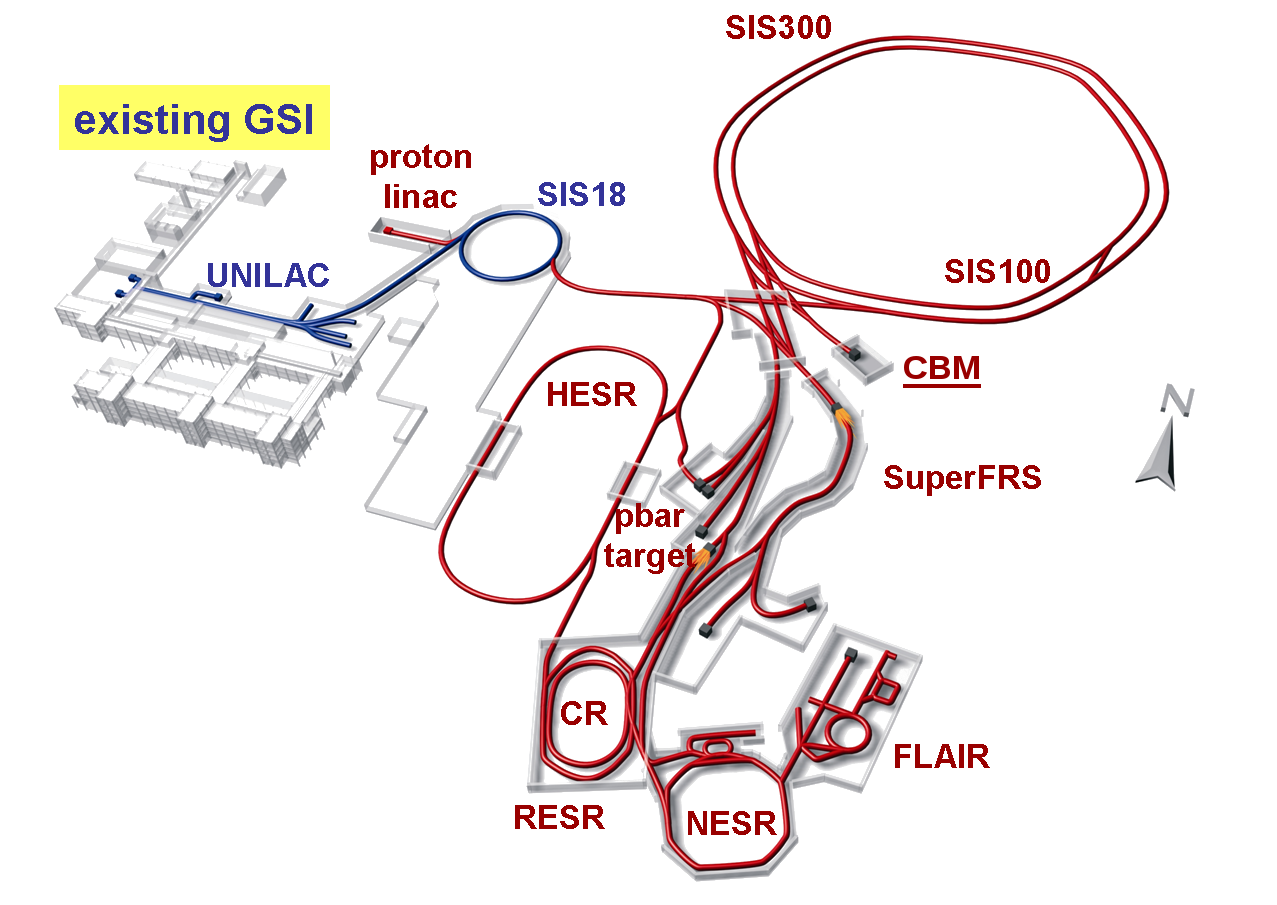
\includegraphics[width=1.0\textwidth]{pictures/FAIR_structure.png}
\caption{Схема FAIR.}
\label{fig:FAIRstructure}
\end{figure}

Синхротроны SIS100/300 имеют магнитную жёсткость 100~Тл$\cdot$м и 300~Тл$\cdot$м. Они способны производить пучки ионов максимальной зарядности от протона до урана с интенсивностью до $10^9$ ионов в секунду и энергией от~2~до~35~\GeVperNucl для тяжёлых ионов.

%Для программы ядерных столкновений SIS100/300 предоставит пучок ядер, имеющий магнитную жёсткость 100 и 300~мТл соответственно, ионов до урана с очень высокой интенсивнотью (до $2 \times 10^9$ ионов в секунду) и энергией от~2~до~35~\GeVperNucl.
%предоставят лёгкие ионы (Z/A=0.5) будут ускоряться до 45~\GeVperNucl, а протоны --- до 90~\GeV.

Ещё одной отличительной особенностью FAIR являтся то, что он будет предоставлять пучок для нескольких (до~4) исследовательсих установок одновременно, позволяя CBM работать с пучком тяжёлых ионов до 4~месяцев в год. На \figref{fig:FAIRstructure3} показана схема предоставления пучка параллельно нескольким экспериментам.
% Описание можно стырить из FAIR_BTR


\begin{figure}[H]
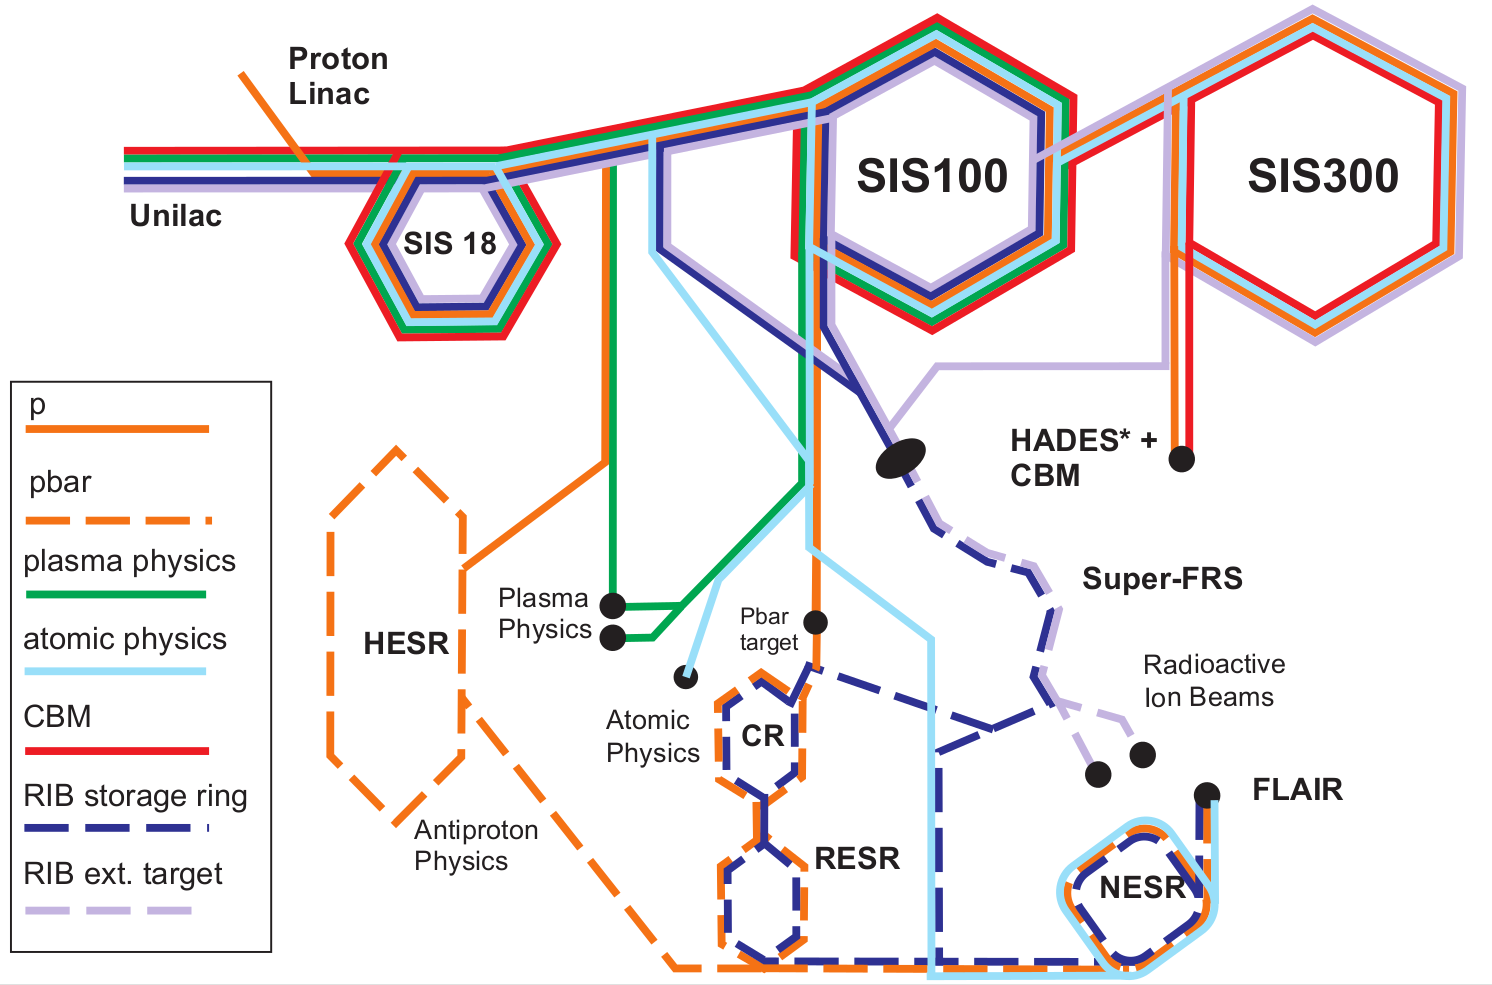
\includegraphics[width=1.0\textwidth]{pictures/FAIR_structure_3.png}
\caption{Схема FAIR.}
\label{fig:FAIRstructure3}
\end{figure}

Широкий диапазон энергий, предоставляемый FAIR, позволит производить ядерную материю при максимальных плотностях, доступных при столкновениях тяжёлых ионов. В соответствии с разными моделями ядерного взаимодействия на раннем этапе центрального Au+Au столкновения при энергии пучка 20~\GeVperNucl ($s_{NN} \approx 6.4$~\GeV) плотность с центре сгустка будет достигать уровня примерно в 12~раз выше обычной ядерной плотности.

%The broad energy range provided by FAIR will allow producing nuclear matter at the maximal net baryon density achievable with heavy ion collisions [8]. As shown in Figure 3, according to various transport models, the density reaches up to about twelve times the normal nuclear matter density in the core and at the early stage of central Au+Au collisions at a beam energy of 20 GeV/nucleon ( (s NN ) ∼ 6.4 GeV). As can be seen in Figure 4, this important feature of the FAIR accelerator is supported by the derived chemical freeze–out parameters that are required to reproduce, within a canonical or grand canonical statistical model, the measured particle yields in central A+A collisions at SIS, AGS, SPS and RHIC energies ( (s NN ) ∼ 2, 5, 20, 200 GeV, respectively) [9]. As the beam energy decreases a clear shift towards lower temperatures and higher μ B occurs.

The identification of multi-strange hyperons, hypernuclei, particles with charm quarks and vector mesons decaying into lepton pairs requires efficient background suppression and very high interaction rates. In order to select events containing those rare observables, the tracks of each collision have to be reconstructed and filtered online with respect to physical signatures. This concept represents a paradigm shift for data taking in high-energy physics experiments: CBM will run without hierarchical trigger system. Self-triggered read-out electronics, a high-speed data processing and acquisition system, fast algorithms, and, last but not least, radiation hard detectors are indispensable prerequisites for a successful operation of the experiment.

\section{Экспериментальная установка CBM}\label{sec:secCbmSetup}

% \textbf{См. английские оригиналы в комментах теха.}

Для выполнения различных измерений CBM будет функционировать в двух конфигурациях --- с мюонным детектором (MUCH) и с детектором черенковских колец (RICH). Схема экспериментальной установки с RICH представлена на \figref{fig:CBM}.

\begin{figure}[H]
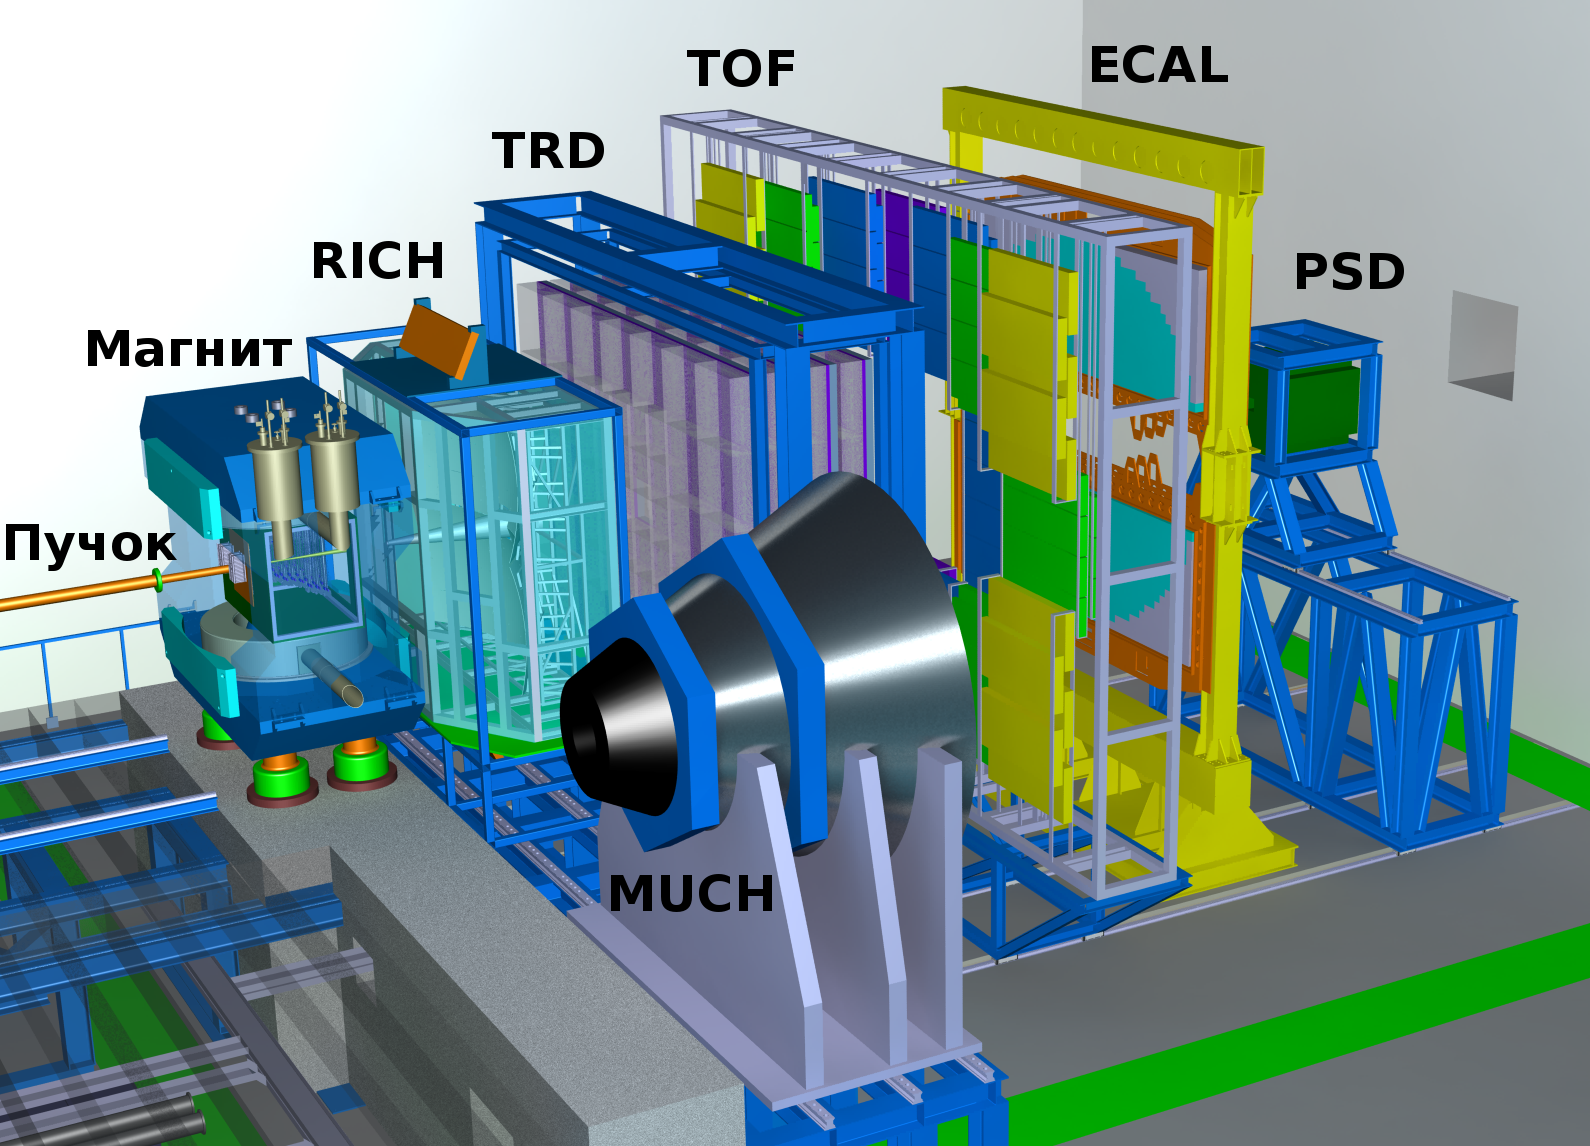
\includegraphics[width=1.0\textwidth]{pictures/1_CBM_SIS100_with_names.png}
\caption{Общий вид экспериментальной установки CBM в конфигурации с RICH.}
\label{fig:CBM}
\end{figure}

Между полюсами сверхпроводящего дипольного магнита~\cite{TDR_Magnet} (см.~\figref{fig:InMagnetBox}) расположена вакуумная камера, содержащая мишень и вершинный микродетектор (MVD)~\cite{MVD_KOZIEL}, выполненный на основе монолитного пиксельного детектора типа MAPS. Ниже по пучку также между полюсами, но уже вне вакуумной камеры, располагаются станции кремниевой трековой системы (STS)~\cite{TDR_STS}, собранные из двухсторонних микростриповых сенсоров. Координатные трековые детекторы MVD и STS предназначены для реконструкции траекторий заряженных частиц, восстановления их импульсов с точностью не хуже 1\% и нахождения вторичных вершин в условиях высокой множественности и плотности частиц.

\begin{figure}[H]
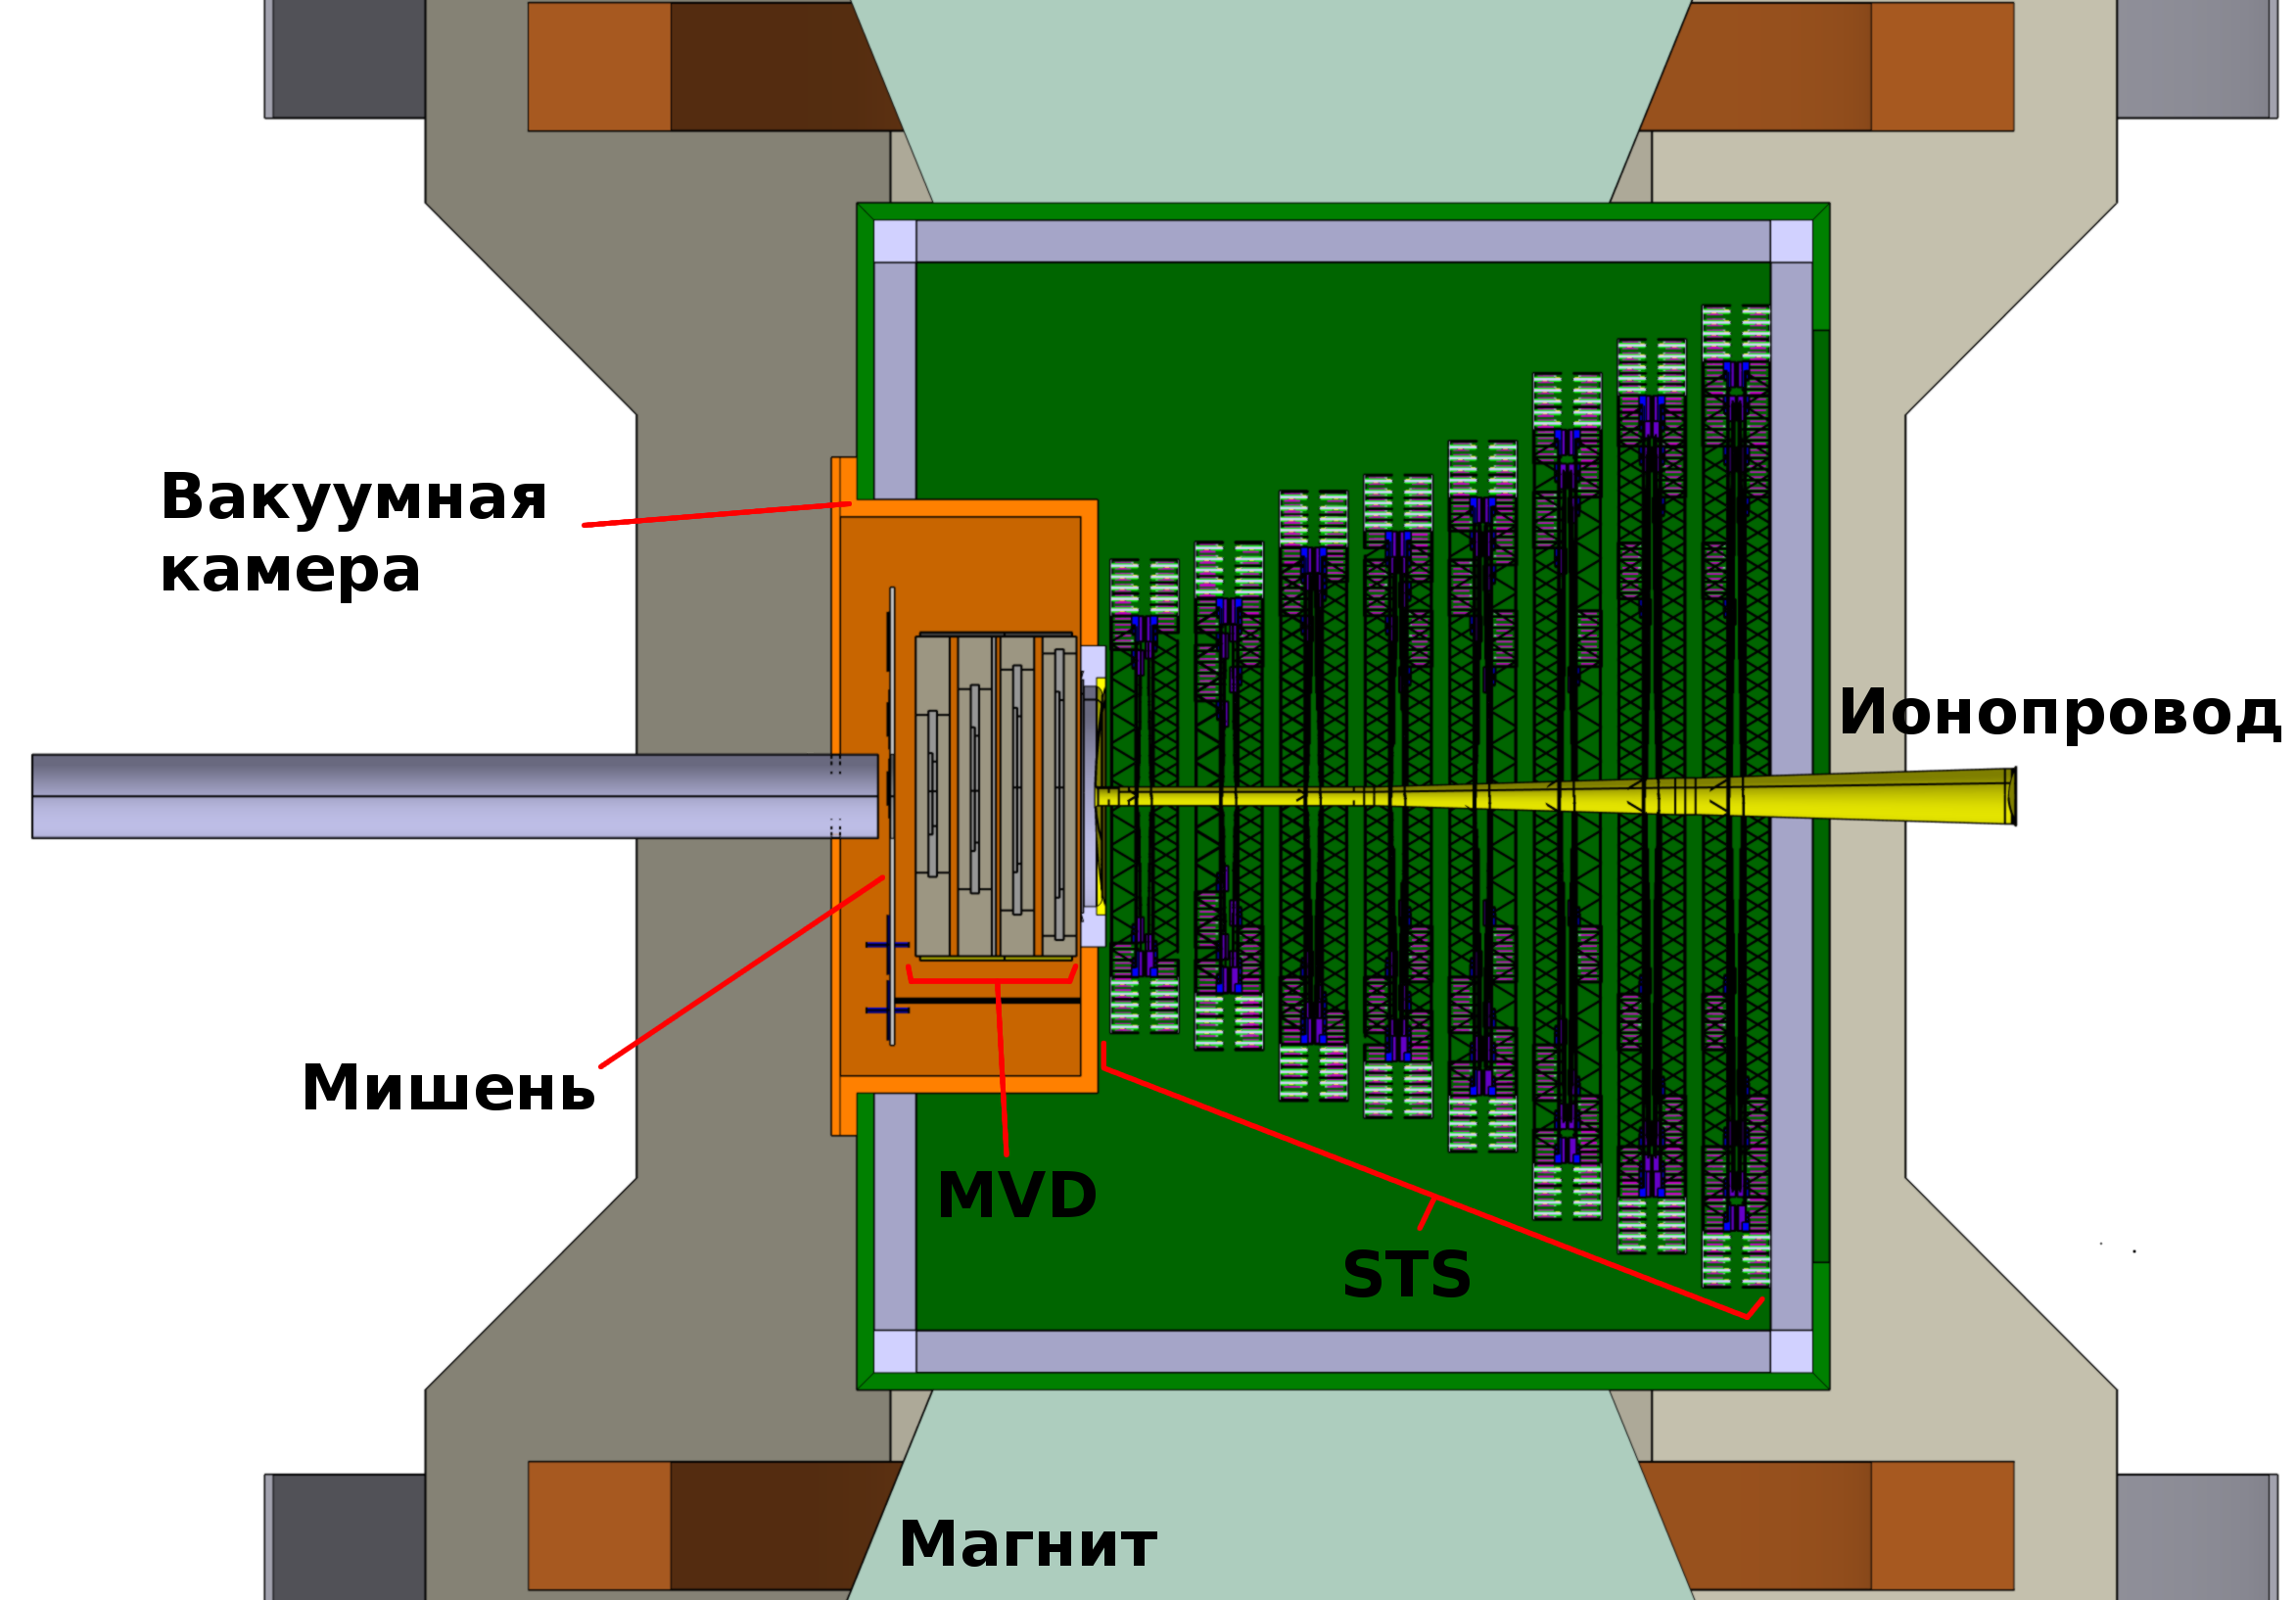
\includegraphics[width=1.0\textwidth]{pictures/CBM_vacuum_chamber_model.png}
\caption{Разрез модели ионопровода, вакуумной камеры и детекторов, расположенных между полюсами мангита.}
\label{fig:InMagnetBox}
\end{figure}

Следом за STS в рассматриваемой конфигурации расположен детектор черенковских колец (RICH)~\cite{TDR_RICH}, предназначенный для идентификации электронов и позитронов в диапазоне импульсов от 0.5~\GeVoverC до 8~\GeVoverC с целью восстановления распадов легких векторных мезонов и $ J / \psi $ частиц. Во второй конфигурации на месте RICH стоит мюонная система (MUCH, показана на \figref{fig:CBM} в положении хранения)~\cite{TDR_MUCH}, предназначенная в первую очередь для исследования частиц, распадающихся по димюонному каналу и состоящая из чередующихся слоев железа и газовых трековых камер~\cite{GEM}.

Детектор переходного излучения (TRD) используется для реконструкции треков частиц и идентификации электронов/позитронов в условиях доминирующего фона от пионов~\cite{TRD}. Для идентификации адронов используется время-пролётный детектор (TOF)~\cite{TDR_TOF}. Электромагнитный калориметр (ECAL) типа ``шашлык'' необходим для регистрации прямых фотонов и фотонов от распада нейтральных мезонов ($ \pi^{0}, \eta $)~\cite{ECAL_KOROLKO}. Детектор непровзаимодействовавших осколков ядер (PSD)~\cite{TDR_PSD} представляет собой сегментированный адронный калориметр и служит для определения центральности столкновения и плоскости реакции путем регистрации ядерных осколков, летящих под малыми углами к пучку.

Далее каждый элемент установки описан чуть подробнее.

% ==========================================================================================
% ==========================================================================================
% ==========================================================================================

\subsection{Вакуумная камера, мишень и ионопровод}\label{sec:secVacChamberPipe}

CBM является экспериментом с фиксированной мишенью. Пучок подводится к установке с помощью ионопровода, который стыкуется с вакуумной камерой, расположенной между полюсами дипольного магнита. Внутри вакуумной камеры находится мишень и вершинный микродетектор MVD. Мишень представляет собой золотую фольгу толщиной порядка ста микрон или набор из нескольких фольг меньшей толщины, разнесённых вдоль оси пучка. Непровзаимодействовавшие ионы налетающего пучка и крупные осколки продолжают движение по ионопроводу за вакуумной камерой.

Планируется, что пучковая труба будет выполнена из алюминия толщиной от 0.3~мм диаметром от 4~см на выходе из вакуумной камеры до 60~см в зоне время-пролётного детектора.

Для измерения момента времени первичного взаимодействия пучка с мишенью, который необходим для измерения времени пролёта вторичных частиц с помощью TOF, вблизи мишени будет расположен стартовый детектор. См. также~\ref{sec:secTOF}.

% ==========================================================================================
% ==========================================================================================
% ==========================================================================================

\subsection{Дипольный магнит}\label{sec:secMagnet}

Основная задача магнита --- разводить в пространстве заряженные частицы для обеспечения возможности их регистрации детекторами, стоящими ниже по пучку. Для этого магнит должен обеспечить максимально равномерное стационарное вертикальное магнитное поле в заданной области пространства, а также минимизировать поле за пределами этого пространства.

Сверхпроводящий магнит.
provides a field integral of 1 Tm

%Конфигурация магнита определяется геометрическим аксептансом эксперимента, который составляет полный 2$\pi$ по азимуту $\phi$) и интервал от $\SI{2.5}{\degree}$ до $\SI{25}{\degree}$ по полярному углу ($\theta$). Мишень, вершинный микродетектор MVD и кремниевая трековая система STS должны располагаться внутри магнитного поля, что диктует требование к размерам 

Design constraints:
Угол раствора от мишени: $\pm \SI{25}{\degree}$ по вертикали и $\pm \SI{30}{\degree}$ по горизонтали.
Магнит должен быть способен переключать полярность.
Конструкция магнита должна подразумевать сборку на месте.
Максимальная нагрузка на пол: 100 тонн/м$^{2}$.
Высота пучка над основанием: 2.7~м.
Магнит должен быть позиционирован с точностью $\pm0.2$~мм по координате и $\pm0.5$~мрад по углу.

Расстояние между полюсами по вертикали 1440~мм, длина вдоль пучка --- сравнительно небольшая --- 1~м.

Съёмные field clamps
Цилиндрические обмотки из NbTi, намотанные на цилиндрическую бобину и охлаждаемые жидким гелием
Термический щит, охлаждаемый газообразным гелием при температуре 50--80 $K$.

Интеграл поля по всей области, где находится STS: 0.972~Tm \todo, следовательно макс. поле $\approx 1 T $, в зависимости от длины магнита.
Отклонение интеграла поля по всему телесному углу по прямым линиям $\leq$ 20\% ($\pm$10\%).

%Field integral within STS detector (along straight lines): 0,972 Tm -> max. Field ≈ 1 T, depending on the magnet length
%Field integral variation over the whole opening angle along straight lines: ≤ 20\% ($\pm$10\%)



%The geometrical acceptance of the CBM detector systems is full 2$\pi$ for azimuth ($\phi$) and from $\SI{2.5}{\degree}$ to $\SI{25}{\degree}$ for polar ($\theta$) angles.



%the free aperture was increased from 1.4m (TDR) to 1.44 m. However, the integral field was decreased in order to keep the nominal current the same as in the TDR.

\begin{figure}[H]
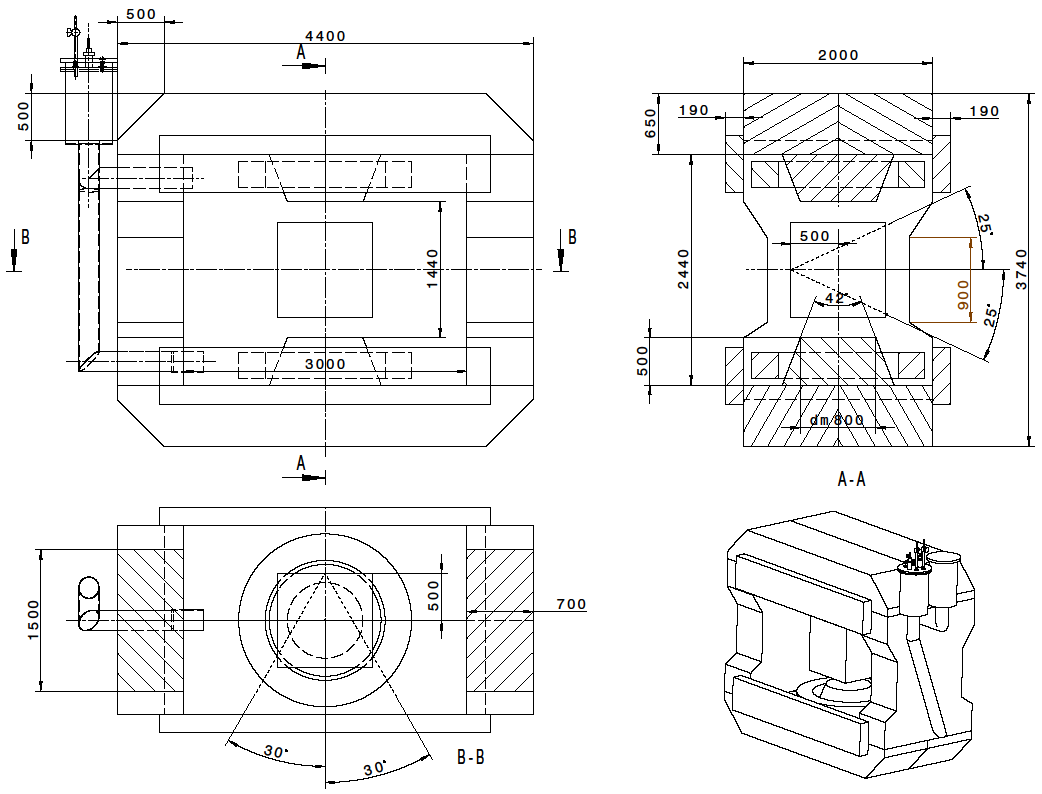
\includegraphics[width=0.98\textwidth]{pictures/Magnet_drawing.png}
\caption{Чертёж магнита.} % из CBM Dipole Detailed Specification из Collaboration Contract between the FAIR GmbH and BINP
\label{fig:MagnetDrawing}
\end{figure}

\begin{figure}[H]
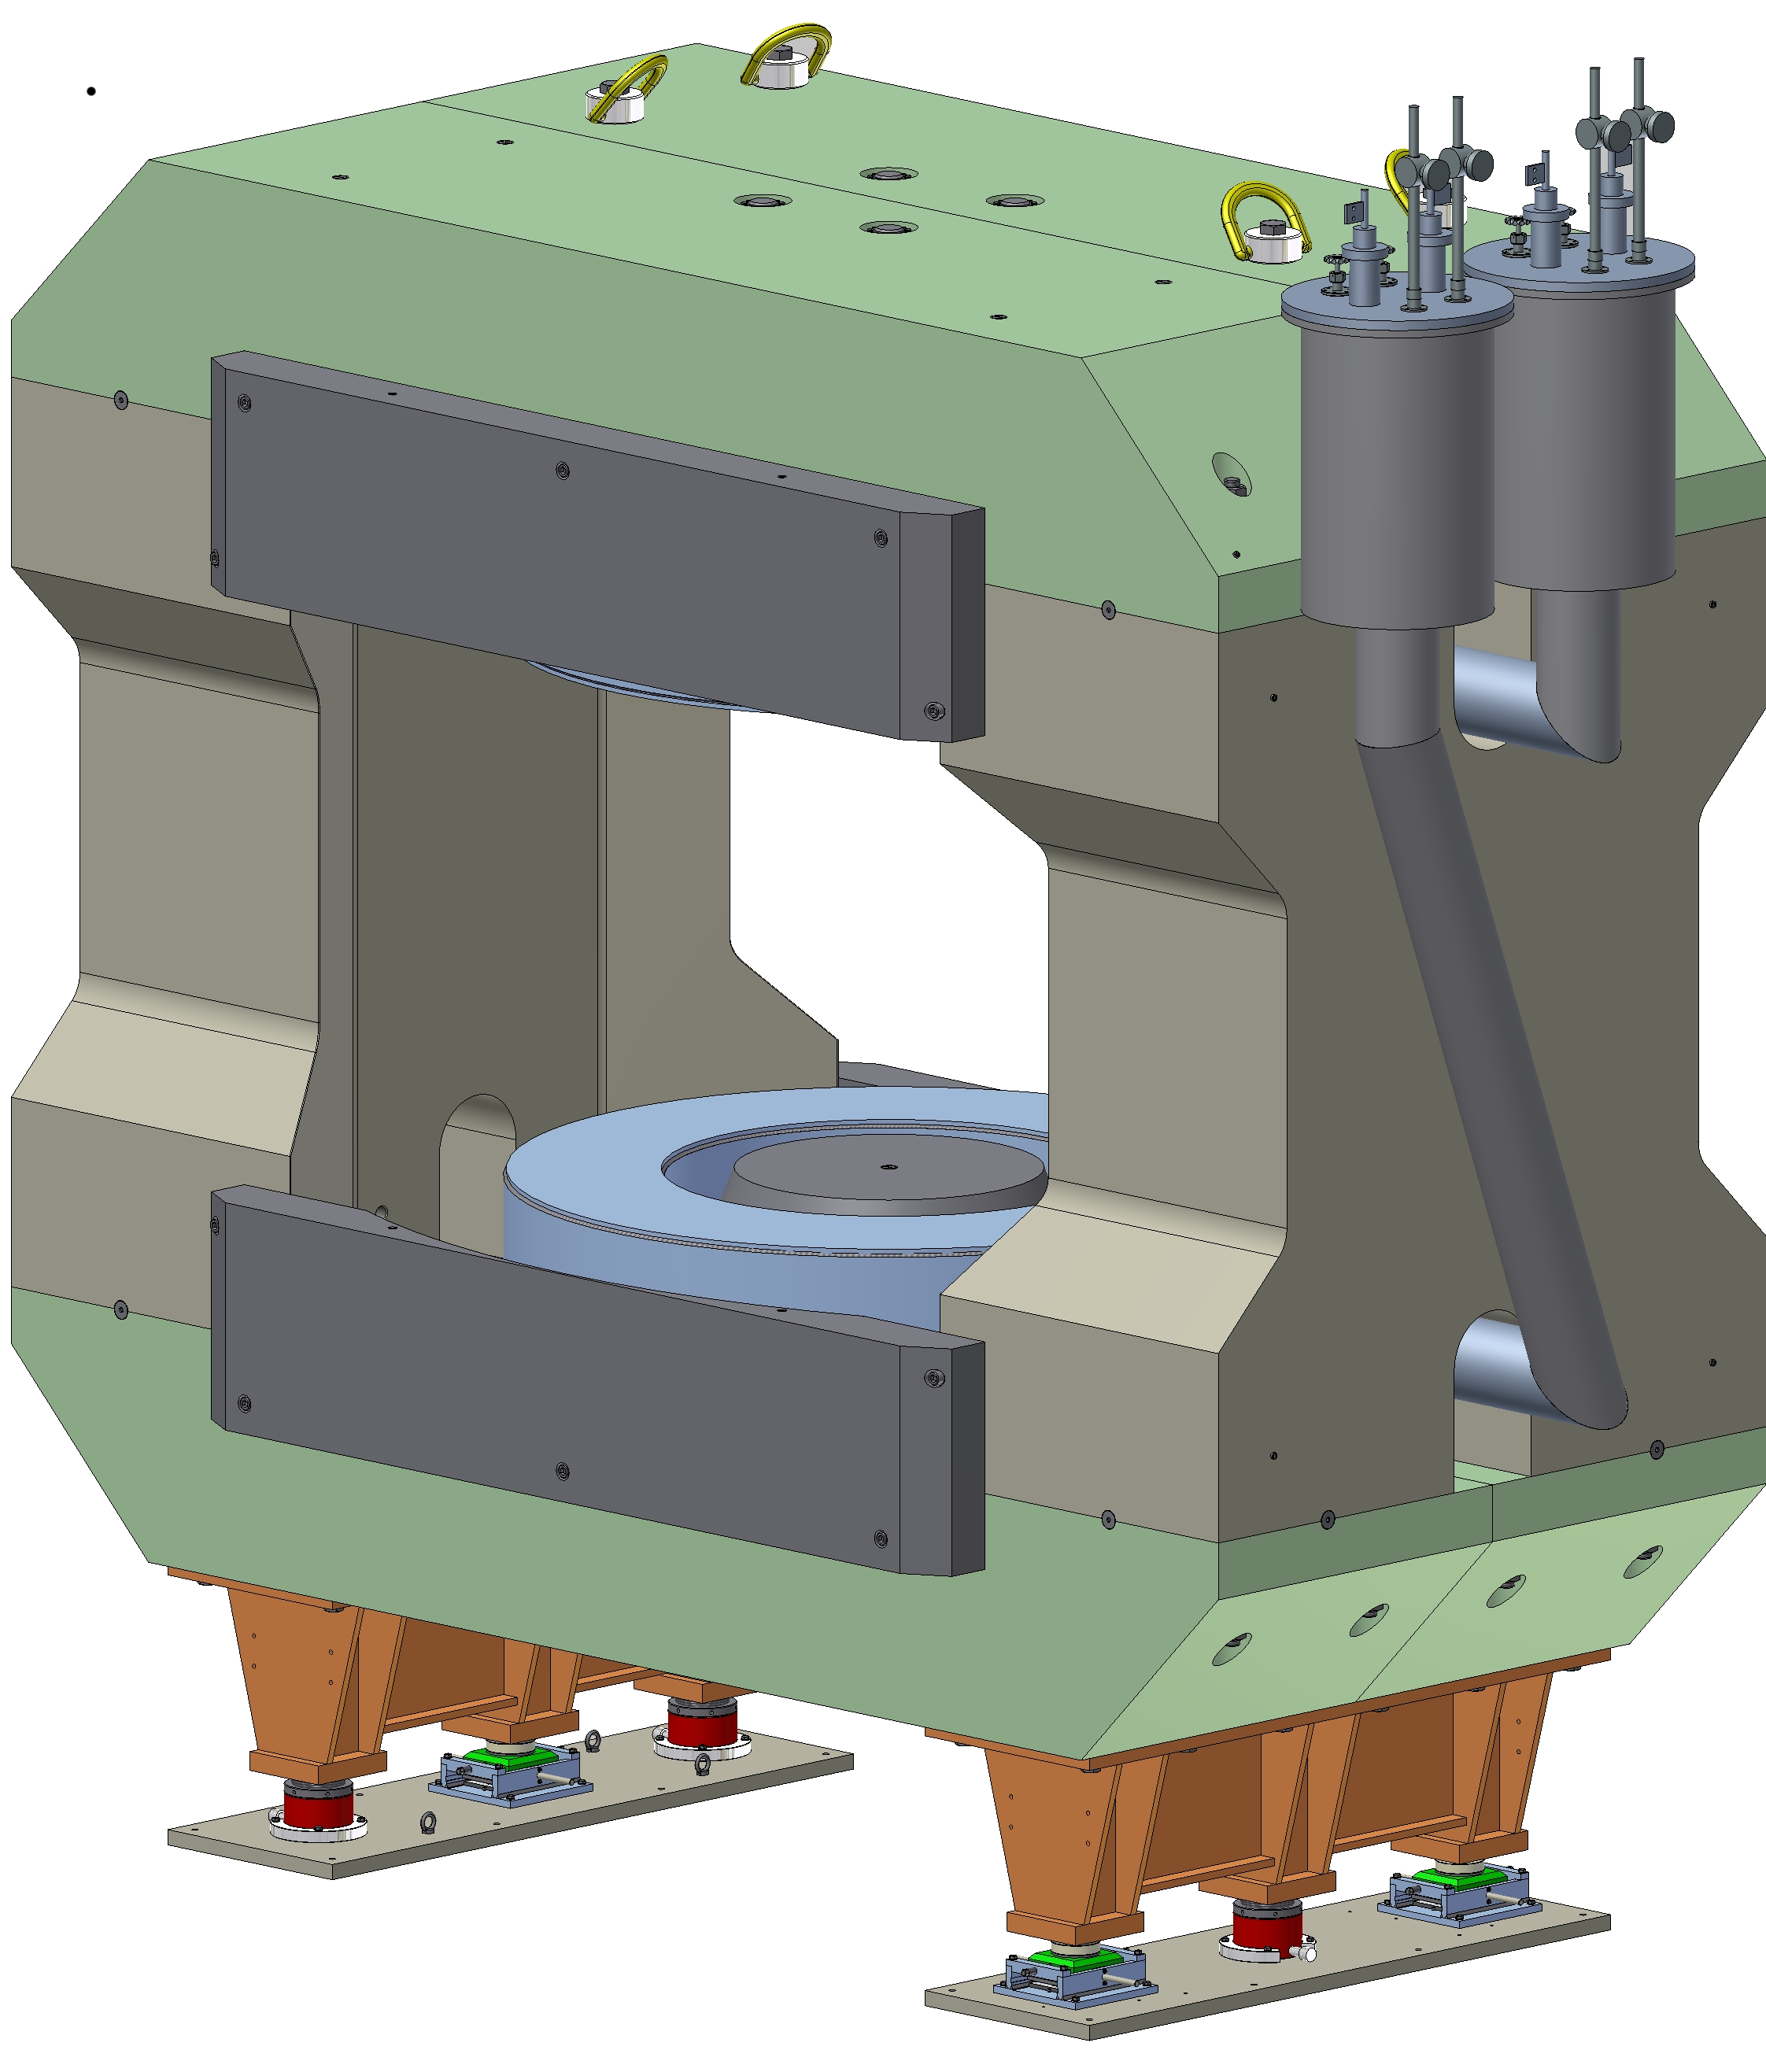
\includegraphics[width=0.7\textwidth]{pictures/CBM_magnet_model.png}
\caption{Модель магнита}
\label{fig:MagnetModel}
\end{figure}

% ==========================================================================================
% ==========================================================================================
% ==========================================================================================

\subsection{Вершинный микродетектор MVD}\label{sec:secMVD}

Вершинный микродетектор (Micro Vertex Detector, MVD) является первым трекинговым устройством установки CBM и расположен внутри вакуумной камеры (см.~\figref{fig:MVD12}). MVD состоит из четырёх двухсторонних станций на расстояниях 5, 10, 15 и 20~см от мишени (вниз по пучку \todo).
MVD улучшает разрешение трековой системы CBM, позволяя таким образом идентифицировать редкие частицы по пространственному отклонению вершины распада. В таблице~\ref{tabl:MVDphys} приведены наблюдаемые, измерение которых возможно за счёт использования MVD.
Помимо этого, широкий геометрический аксептанс MVD вносит значительный вклад в трекинг частиц с низким импульсом, что повышает способность системы к подавлению фона при измерении распадов по диэлектронному каналу.

\begin{table}[H]
\caption{}
\label{tabl:MVDphys}
\begin{tabular}{ | p{0.22\linewidth} | p{0.22\linewidth} | p{0.22\linewidth} | p{0.22\linewidth} | }
\hline
\textbf{Частица} & \textbf{Канал} \newline \textbf{распада} & \textbf{Коэф.} \newline \textbf{ветвления} & \textbf{Время жизни, c$\tau$} \\
\hline
$\mathbf{D^{+}}$ & $K^{-} + \pi^{+} + \pi^{+}$ & 9\% & $315 \mu$м \\
\hline
$\mathbf{D^{0}}$ & $K^{-} + \pi^{+}$ & 4\% & $124 \mu$м \\
\hline
$\mathbf{\lambda_{C}}$ & $p + K^{-} + \pi^{+}$ & 5\% & $62 \mu$м \\
\hline
\end{tabular}
\end{table}

MVD будет построен на основе активных пиксельных КМОП (CMOS) сенсоров (Monolithic Active Pixel Sensors, MAPS) толщиной $50 \mu$м, имеющих пространственное разрешение $3.5 \mu$м. Данная технология, вместе с правильно подобранными материалами для опорных структур и кабелей, позволяет получить вклад материала порядка 0.3\% $X_{0}$ для первой станции.

%The Micro Vertex Detector (MVD) is the first tracking device, with its first station located only 5 cm downstream of the fixed target. It will improve the vertex resolution of the CBM tracking system, to be able to identify rare particles by the spatial displacement of their decay vertices. In addition, the large geometrical acceptance of the MVD will significantly contribute to the tracking of low-momentum particles and thus improve the background suppression capability in dielectron measurements. The MVD employs highly granular, 50 μm thin CMOS Pixel Sensors. Together with high performance carrier materials and cable technology, this results in a material budget of only 0.3\% $X_{0}$ for the first station.

%The MVD will rely on CMOS Monolithic Active Pixel Sensors (MAPS) which provide the necessary radiation tolerance, a spatial resolution of 3.5μm, 50μm thickness, and advanced on‐chip data processing.

%The MVD will operate in the target vacuum to obtain the best possible vertex resolution.

На~\figref{fig:MVD3} показано устройство сенсора MVD.
На части чипа сенсора реализована предварительная обработка сигнала.
%A part of the sensor chip hosts data processing circuits. The second sensor covers this surface.
По тонким гибким шлейфам к сенсорам подводится питание и осуществляется считывание.
%Thin flex print cables serve to bias and readout the sensors.
Детектор MVD будет испытывать значительные радиационные нагрузки, поэтому особое внимание уделяется охлаждению активных сенсоров. 
За пределами геометрического аксептанса расположены платы передней электроники и система жидкостного охлаждения, соединённая с сенсорами с помощью CVD алмазной пластины.
%A liquid cooled heat sink located outside the detector acceptance hosts front end boards and absorbs the dissipated power of the system.
Данные (800~Mbps/сенсор) считываются радиационно-стойкими пассивными платами передней электроники и отправляются в DAQ-систему по стандарту HADES-TRB3.
%The data of the sensors will be received by a radiation tolerant, passive front end board. It sends the data (800 Mbps/sensor) to a DAQ‐system based on the HADES‐TRB3 standard.

\textbf{Какие-то слова о системе считывания, пока что аналогичной той, что используется в CBM.}
Временное разрешение $5 \mu$с \todo \todo \todo

\begin{figure}[H]
\begin{minipage}[b]{0.495\textwidth}
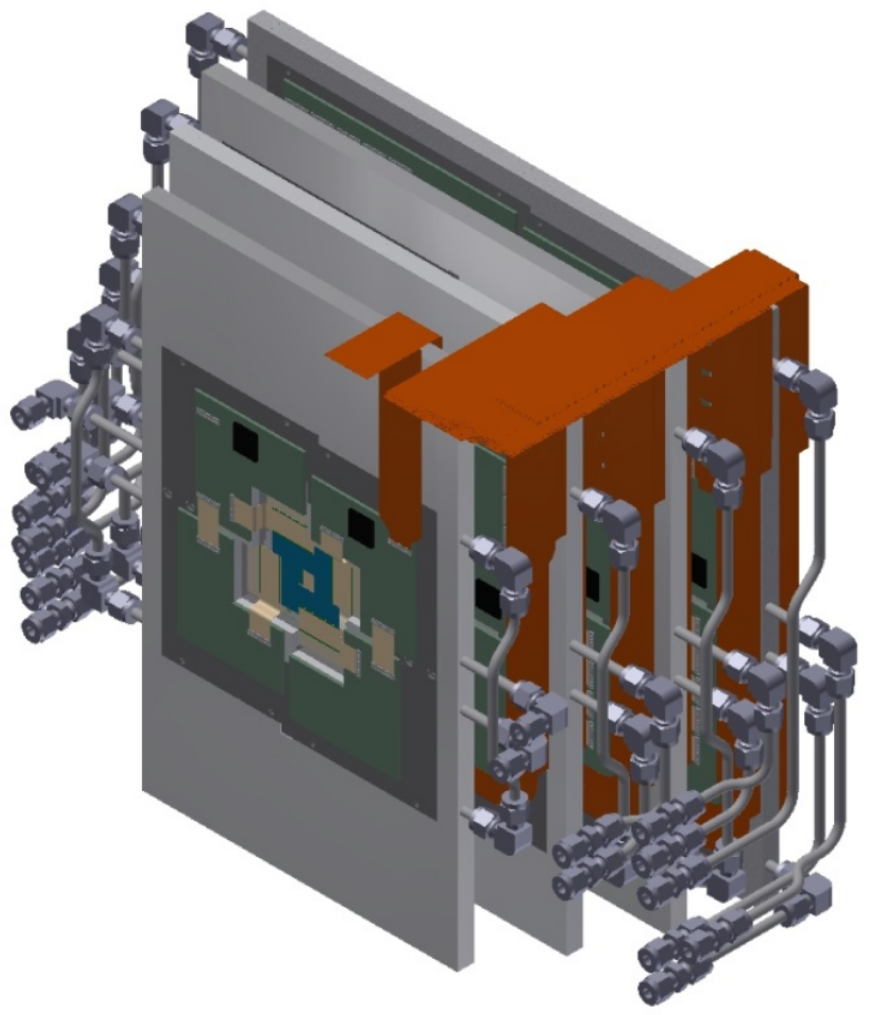
\includegraphics[width=1.0\textwidth]{pictures/MVD_1.png}
\end{minipage}
\hspace{0.01\textwidth}
\begin{minipage}[b]{0.495\textwidth}
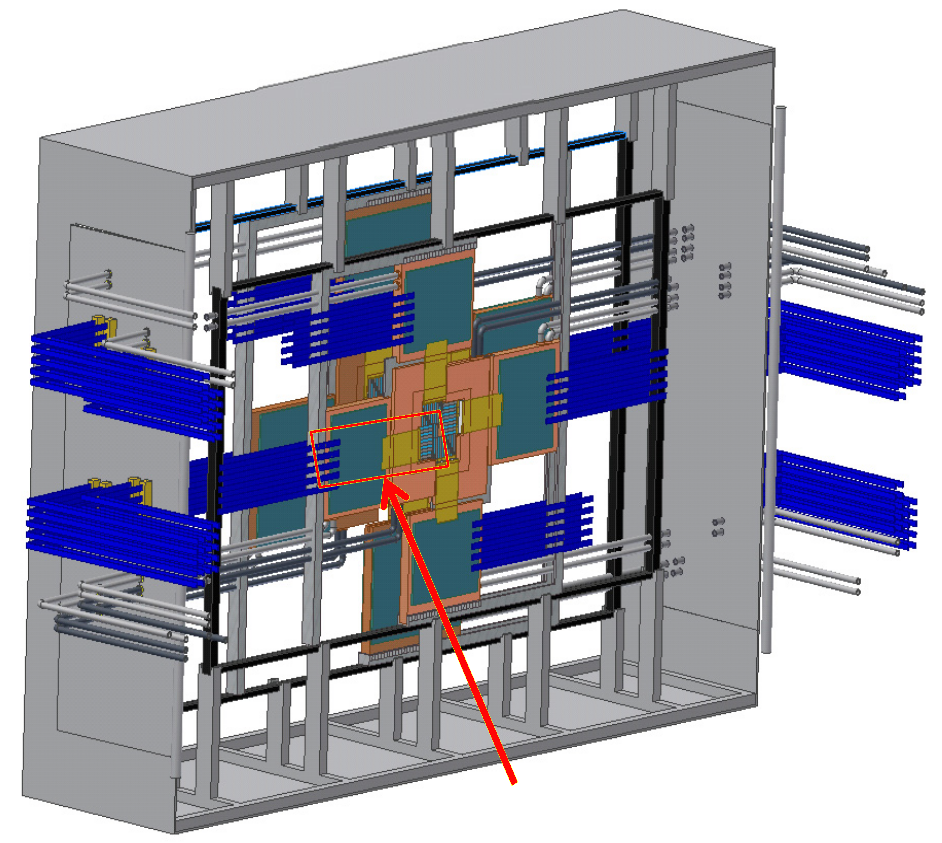
\includegraphics[width=1.0\textwidth]{pictures/MVD_2.png}
\end{minipage}
\caption{}
\label{fig:MVD12}
\end{figure}

\begin{figure}[H]
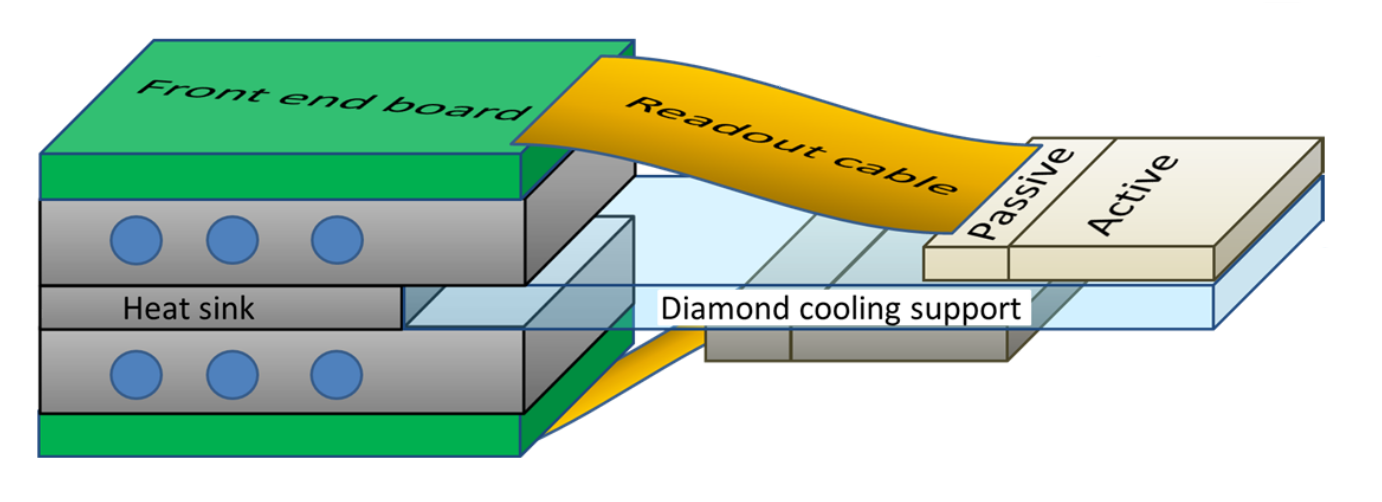
\includegraphics[width=1.0\textwidth]{pictures/MVD_3.png}
\caption{}
\label{fig:MVD3}
\end{figure}

% ==========================================================================================
% ==========================================================================================
% ==========================================================================================

\subsection{Кремниевая трекинговая система STS}\label{sec:secSTS}

% From CBM STS TDR Summary

Задача кремниевой трековой системы (Silicon Tracking System, STS) --- измерение траекторий и импульсов заряженных частиц, вылетающих из точки взаимодействия пучка тяжёлых ионов с мишенью. Для выполнения физической программы CBM необходима частота взаимодействий до 10~МГц, при том что в одном взаимодействии будет рождаться до 1000 заряженных частиц. Реконструкция треков должна выполняться с эффективностью порядка 95\% и разрешением по импульсу порядка $\Delta p / p = 1\%$. Для удовлетворения перечисленных требований STS должна состоять из 8~слоёв кремниевых микростриповых сенсоров, расположенных внутри поля от дипольного магнита на растоянии от 30~см до 100~см от точки взаимодействия вниз по пучку с шагом 10~см.

%The detector system’s task is to measure the trajectories and momenta of charged particles originating from the interactions of heavy-ion beams with nuclear targets. Up to 1000 charged particles are produced per interaction, at rates up to 10 MHz to enable CBM physics with rare observables. The track reconstruction has to be achieved with 95\% efficiency and a momentum resolution ∆p/p = 1\%. These requirements can be fulfilled with a tracking system of 8 low-mass layers of silicon microstrip sensors located at distances between 30 cm and 100 cm downstream of the target inside the magnetic dipole field.

Сенсоры будут монтироваться на легкую механическую опору в виде карбоновых ферм. Считывание будет осуществляться по многоканальным микро-кабелям самотриггирующейся электроникой, расположенной по краям станций вместе с линиями охлаждения и другими инфраструктурными подсистемами.
Многослойные полиамид-алюминиевые кабели будут иметь толщину порядка $100 \mu$м.
Стерео-угол между стрипами равен \SI{7.5}{\degree}.
Микростриповые сенсоры будут двухсторонними, шаг между стрипами $58 \mu$м, длина стрипов от 20~до~60~мм, а толщина кремния $300 \mu$м. По текущим оценкам максимальная неионизирующая доза в CBM для сенсоров, расположенных ближе всего к пучку, не будет превышать $10^{14}$ $n_{eq}$ см$^{-2}$. STS будет работать в термостатическом корпусе, обеспечивающем постоянную температуру около \SI{-5}{\degreeCelsius}. Тепло, рассеиваемое считывающей электроникой, отводится с помощью $CO_{2}$ системы охлаждения. Механические опоры детектора и соединения спроектированы так, чтобы была возможность заменить отдельный модуль системы не отсоединяя остальные.

%The sensors are mounted onto lightweight mechanical support ladders and read out through multi-line micro-cables with fast self-triggering electronics at the periphery of the stations where cooling lines and other infrastructure can be placed. The micro-cables will be built from sandwiched polyimide-Aluminum layers of several 10~$\mu$m thickness. The microstrip sensors will be double-sided with a stereo angle of \SI{7.5}{\degree}, a strip pitch of 58~$\mu$m, strip lengths between 20 and 60 mm, and a thickness of 300 $\mu$m of silicon. According to the CBM running scenario the maximum non-ionizing dose for the sensors closest to the beam line does not exceed $10^{14}$ $n_{eq}$ см$^{-2}$. The STS is operated in a thermal enclosure that keeps the sensors at a temperature of about \SI{-5}{\degreeCelsius}. The heat dissipated in the read-out electronics is removed by a $CO_{2}$ cooling system. The mechanical structure of the detector system including the service and signal connections is designed such that single detector ladders can be exchanged without disconnecting and removing more than one detector station.

\begin{figure}[H]
\begin{minipage}[b]{0.495\textwidth}
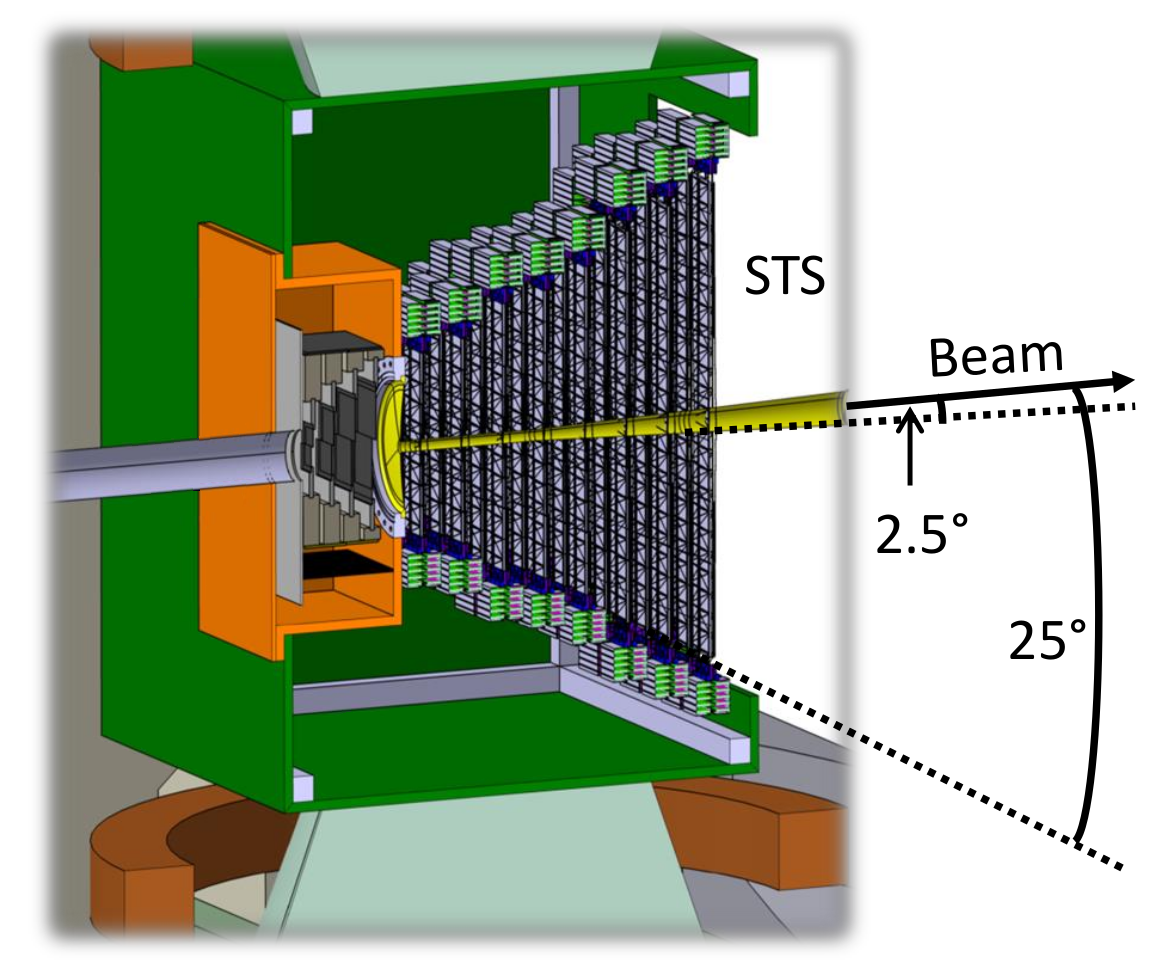
\includegraphics[width=1.0\textwidth]{pictures/STS_1.png}
\end{minipage}
\hspace{0.01\textwidth}
\begin{minipage}[b]{0.495\textwidth}
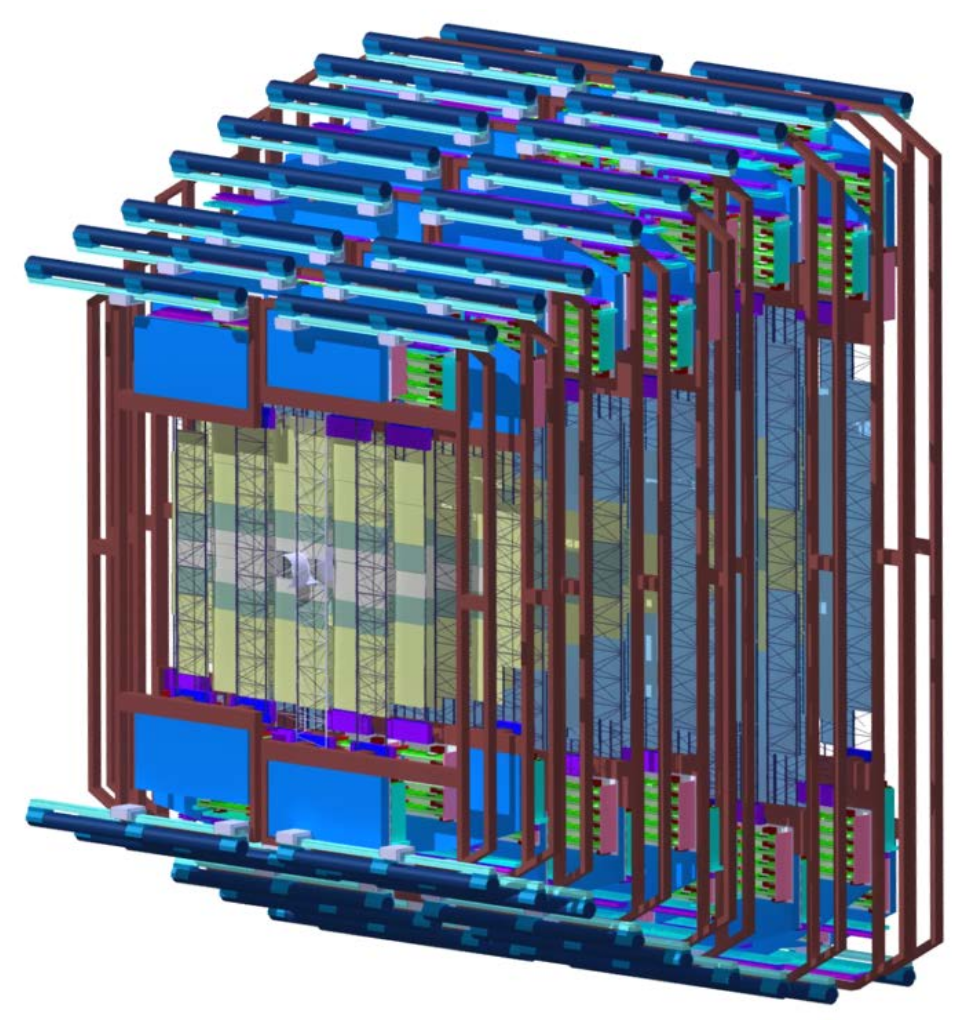
\includegraphics[width=1.0\textwidth]{pictures/STS_3.png}
\end{minipage}
\caption{}
\label{fig:STS12}
\end{figure}

Считывание STS будет осуществляться специально разработанной электроникой, в основе которой лежит чип STS-XYTER.
Чувствительный к амплитуде.
Столько-то бит в АЦП.
Такие-то параметры по времени.
Столько-то каналов.

% ==========================================================================================
% ==========================================================================================
% ==========================================================================================


\subsection{Детектор черенковских колец RICH}\label{sec:secRICH}

По той причине, что в столкновении тяжёлых ионов рождается огромное количество заряженных $\pi$-мезонов, возникает необходимость идентифицировать электроны и позитроны

Детектор черенковских колец (Ring Imaging CHerenkov detector, RICH) решает задачу идентификации частиц в диапазоне импульсов от \todo до 8--10~\GeVoverC.
В паре с детектором переходного излучения TRD, покрывающем более высокие импульсы, RICH позволяет идентифицировать сигнальные электроны от лёгких векторных мезонов и $J/\psi$.

Для получения дилептонных спектров на SIS300 требуется фактор \todo подавления пионов порядка 10000, что осуществимо при совместном применении TRD и RICH, причём фактор \todo подавления пионов последнего должен составлять как минимум 100.

В случае SIS100 

CBM RICH имеет $CO_{2}$ радиатор, который характеризуется коэффициентом преломления $n=1.00045$ при $T=0$ и $p=1$ атм.
Порог черенковского свечения для пионов составляет $p=4.65$~\GeVoverC.

% ==========================================================================================
% ==========================================================================================
% ==========================================================================================


\subsection{Мюонная система MUCH}\label{sec:secMUCH}

%From CBM MUCH TDR:

Мюонная система (MUon CHambers, MUCH) необходима для идентифиации мюонных пар, рождённых в высокоэнергетичных столкновениях тяжёлых ионов в диапазоне энергий пучка от~4~до~40~\GeVperNucl. Измерение лептонных пар является одним из центральных пунктов физической программы CBM, так как они несут информацию о состоянии материи внутри фаербола. В области низких инвариантных масс дилептоны предоставляют информацию о модификации векторных мезонов ``в среде'', что является многообещающей наблюдаемой о восстановлении киральной симметрии. В области средних инвариантных масс в спектре дилептонов преобладает termal \todo радиация от фаербола, которая говорит о его температуре. В области инвариантных масс около 3~\GeVoverC$^{2} $ дилептоны представляют собой подходящий инструмент для изучения аномального подавления чармония в фазе деконфайнмента. В эксперименте CBM для получения полной картины о дилептонной физике будут измеряться как электроны, так и мюоны.

%The MuCh system is designed to identify muon pairs which are produced in high-energy heavy-ion collisions in the beam energy range from~4~to~40~AGeV. The measurement of lepton pairs is a central part of the CBM research program, as they are very sensitive diagnostic probes of the conditions inside the fireball. At low invariant masses, dileptons provide information on the in-medium modification of vector mesons which is a promising observable for the restoration of chiral symmetry. At intermediate invariant masses, the dilepton spectrum is dominated by thermal radiation from the fireball reflecting its temperature. At invariant masses around $ 3 GeV/c^{2} $, dileptons are the appropriate tool to study the anomalous charmonium suppression in the deconfined phase. In the CBM experiment both electrons and muons will be measured in order to obtain a consistent and comprehensive picture of the dilepton physics.

Основной сложностью при измерении мюонов в столкновениях тяжёлых ионов при энергиях пучка, предоставляемых FAIR, является идентификация мюонов с низким импульсом в среде с очень высокой плотностью частиц. Стратегия, выбранная CBM, заключается в том, чтобы выполнять трекинг в системе с адронными абсорберами и выполняться идентификацию мюонов в зависимости от импульса. По этой причине мюонная система будет выполнена в виде последовательности адронных абсорберов и трекинговых станций. Адронные абсорберы различаются по толщине и материалу, а трекинговые станции состоят из троек детекторов, выполненных по различным технологиям. MUCH будет расположен за дипольным магнитом, в том же месте, где стоит RICH в электронной конфигурации CBM. Чтобы уменьшить количество мюонов от слабых распадов пионов и каонов, система из абсорберов и детекторов должна быть максимально компактна.

%The experimental challenge for muon measurements in heavy-ion collisions at FAIR energies is to identify low-momentum muons in an environment of high particle densities. The CBM strategy is to track the particles through a hadron absorber system, and to perform a momentum-dependent muon identification. This concept is realized by an instrumented hadron absorber, consisting of staggered absorber plates and tracking stations. The hadron absorbers vary in material and thickness, and the tracking stations consist of detector triplets based on different technologies. The MuCh system is placed downstream of the dipole magnet hosting the Silicon Tracking System (STS) which determines the particle momentum. In order to reduce the number of muons from pion and kaon weak decays, the absorber/detector system has to be as compact as possible.

Мюонная система будет строиться поэтапно соответственно энергиям пучка, предоставляемым ускорителем. В рамках FAIR MSV (\todo ссылка) синхротрон SIS100 будет выдавать пучок тяжёлых ионов с энергией до 14~\GeVperNucl и протонный пучок с энергией до 29~\GeVperNucl. Две первые версии MUCH (SIS100-A и SIS100-B) будут состоять из~3~и~4~станций соответственно, что подходит для измерения лёгких векторных мезонов в столкновениях при 4--6~\GeVperNucl и 8--14~\GeVperNucl соответственно. Третья версия MUCH (SIS100-C) будет оборудована дополнительным железным абсорбером толщиной 1~м для того, чтобы идентифицировать чармоний при самых высоких энергиях SIS100. 
По введении в эксплуатацию SIS300 мюонная система будет обновлена введением дополнительной станции абсорера и детектора для измерения векторных мезонов с низкой массой (low-mass vector mesons \todo) и чармония при энергиях пучка более 14~\GeVperNucl (версии SIS300-A и SIS300-B).

%The MuCh system will be built in stages which are adapted to the beam energies available. Within the FAIR modularized start version the SIS100 ring will provide heavy ion beams with energies up to 14~AGeV, and proton beams up to 29~GeV. The first two versions of MuCh (SIS100-A and SIS100-B) will comprise of~3~and~4 stations suitable for the measurement of low-mass vector mesons in $ A + A $ collisions at 4-6~AGeV and 8-14~AGeV, respectively. The third version of the MuCh system (SIS100-C) will be equipped with an additional iron absorber of 1~m thickness in order to be able to identify charmonium at the highest SIS100 energies.
%The absorber slices will be built only once so that they could be rearranged properly to obtain required absorber thicknesses.
%Once SIS300 is operational, we will upgrade the MuCh system further by inserting additional absorbers and detector stations for the measurement of low-mass vector mesons and charmonium at beam energies above 14~AGeV (MuCh versions SIS300-A and SIS300-B).

\begin{figure}[H]
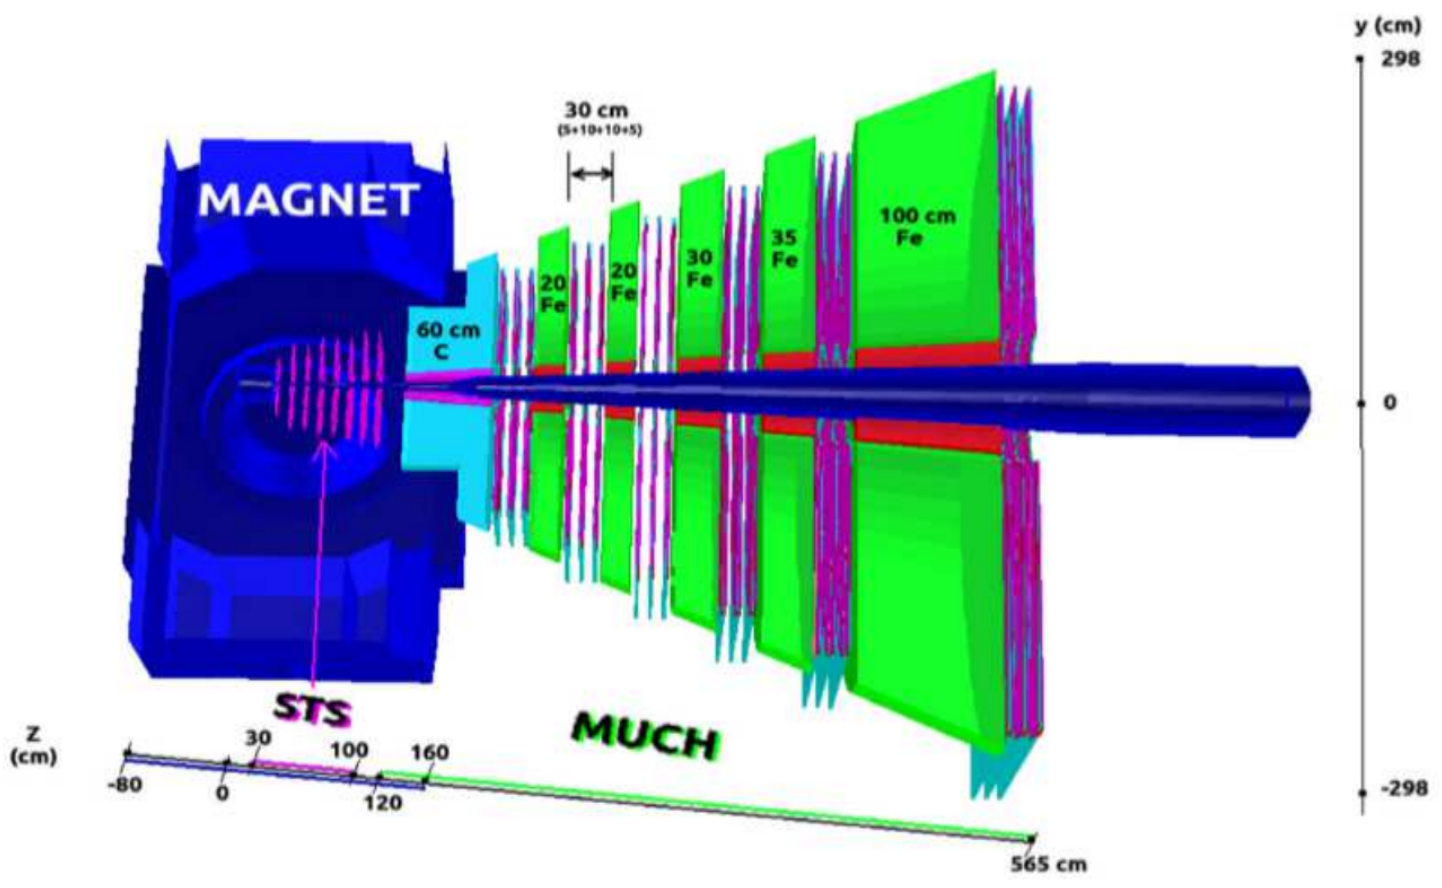
\includegraphics[width=1.0\textwidth]{pictures/MUCH.png}
\caption{Схема расположения станций мюонной системы.}
\label{fig:MUCH}
\end{figure}

\begin{figure}[H]
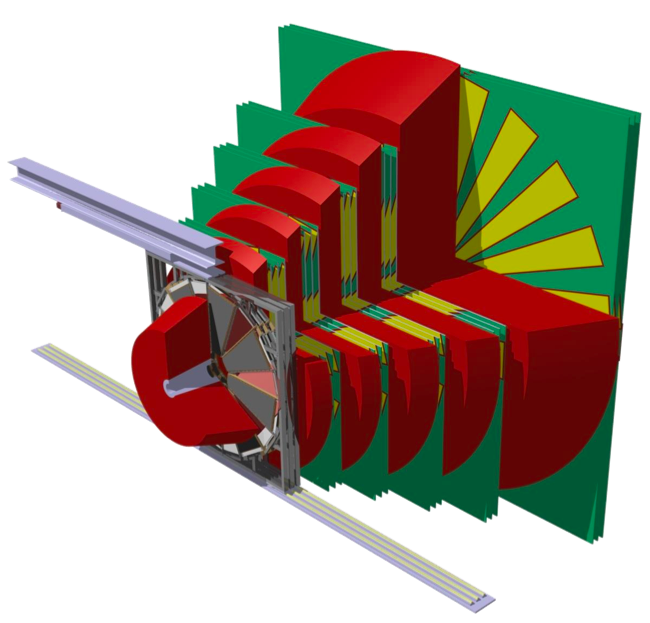
\includegraphics[width=0.6\textwidth]{pictures/CBM_MUCH_model.png}
\caption{Модель мюонной системы MUCH.}
\label{fig:MUCH2}
\end{figure}

% ==========================================================================================
% ==========================================================================================
% ==========================================================================================

\subsection{Детектор переходного излучения TRD}\label{sec:secTRD}

Основная задача детектора переходного излучения (Transition Radiation Detector, TRD) --- идентифицировать электроны с импульсом более 1~\GeVoverC для того чтобы расширить возможности детектора RICH по идентификации частиц в диапазоне импульсов около 5~\GeVoverC.
Такая идентификация должна быть достигнута при коэффициенте подавления пионов порядка 10--20 для получения возможности измерения диэлектронов в диапазоне масс от $\rho$ и $\omega$ и выше J/$\psi$.
Благодаря способности идентифицировать заряженные частицы за счёт их известного энерговыделения детектор TRD также предоставит ценную информацию при регистрации ядерных осколков.
Это особенно важно для отделения, например, дейтронов от $ ^{4}He $, которое не может быть достигнуто с помощью одного только детектора TOF.

%The main task of the TRD is to identify electrons above momenta of 1 GeV/c and thus to extend the electron identification capabilities of the Ring Image CHerenkov (RICH) detector above momenta of p ∼ 5 GeV/c. This identification has to be achieved with a pion suppression factor in the range 10 – 20, in order to allow for a measurement of dielectrons in the mass range from below the ρ and ω masses to beyond the J/ψ mass with a good signal-to-background ratio. Due its capability to identify charged particles via their specific energy loss, the TRD in addition will provide valuable information for the measurement of nuclear fragments. This is in particular important for the separation of, e.g, deuterons and 4 He, which cannot be achieved using a time-of-flight measurement alone.

Указанные требования могут быть удовлетворены применением многопроволочных пропорциональных камер (MWPC) на основе $ Xe/CO_{2} $ с связке с подходящим радиатором. Базовая версия CBM TRD оснащена MWPC с симметричной зоной усиления толщиной 3.5~мм + 3.5~мм и далее областью дрейфа толщиной 5~мм, наличие которой увеличивает вероятность поглащения фотона переходного излучения в активном газовом объёме. Такая геометрия обеспечивает эффективное и быстрое формирование выходного сигнала
Высокая эффективность детектора достигается минимизацией материала между радиатором и газом.

%These requirements can be fulfilled with Xe/CO 2 based Multi-Wire Proportional Chambers (MWPC) detector in combination with an adequate radiator. The default MWPC for the CBM-TRD is composed of a symmetric amplification area of 3.5 + 3.5 mm thickness, followed by a 5 mm drift region to enhance the TR-photon absorption probability in the active gas volume. This geometry provides also efficient and fast signal creation, as well as readout, with timescales below 200 μs per charged particle track. The performance of the detector is optimized by reducing the material budget between radiator and gas volume to a minimum.

Базовая версия CBM TRD предполагает одну станцию, состоящую из четырёх слоёв.
Она будет расположена между детекторами RICH и TOF, таким образом ***
TRD будет использоваться как дополнительная трекинговая станция, расположенная за последним абсорбером MUCH, в мюонной конфигурации CBM.

%The baseline design of the TRD foresees one station composed of four detector layers.
%It will be positioned between the RICH and the Time-Of-Flight (TOF) detector and thus allows to reduce the background in the TOF resulting from track mismatches by providing additional position information for high precision tracking between Silicon Tracking System (STS) and TOF.
%The TRD will also be used as tracking station behind the last absorber of the MUCH detector in the muon configuration of CBM.

% ==========================================================================================
% ==========================================================================================
% ==========================================================================================

\subsection{Время-пролётный детектор TOF}\label{sec:secTOF}

\textbf{В TDR есть неплохие картинки (см. стр 74).}

%From CBM TOF TDR:

Основная задача время-пролётного детектора (Time Of Flight detector, TOF) --- измерять момент времени прихода заряженных частиц, чтобы провести идентификацию после сопоставления хита TOF с соответствующим треком кремниевой трековой системы STS.

%The detector system’s prime task is to measure the arrival time of charged particles to allow for their identification after having matched the TOF - hit with the corresponding STS track obtained from the CBM silicon tracking system (STS). 

Так как CBM представляет собой эксперимент с фиксированной мишенью, поток заряженных частиц сильно зависит от направления. Стена TOF будет собрана из модулей различной гранулярности и выполненных с разными требованиями к допустимой частоте. Чтобы иметь достаточную степень разделения, особенно для идентификации заряженных каонов, необходимо расстояние до 10~м и временное разрешение порядка 80~пс, что приводит к требуемому размеру TOF около 12$\times$9~м$^2$. Чтобы достичь указанного временного разрешения детектор должен быть оборудован электроникой с гарантированным временным разрешением лучше 60~пс и эффективностью лучше 95\%.

%Since CBM is operated in fixed target mode the flux of charged particles is strongly varying with the polar angle. A modular TOF wall is proposed whose elements, called modules in the following, are adapted to the granularity and rate requirements. To allow for sufficient separation power especially for the identification of charged kaons, distances of up to 10 m and a system time resolution of 80 ps are necessary leading to an overall size of the TOF - wall of approx. 12$\times$9 m2 . To achieve the overall time resolution this area needs to get instrumented with timing detectors with an intrinsic timing resolution better than 60 ps and an efficiency better than 95\%.

Предлагается построить CBM TOF на основе современных (по-русски \todo) (Multigap Resistive Plate Chambers, MRPC). Базовый элемент этого robust \todo детектора --- пачка резистивных пластин из стекла или керамики, которые разделены тонким зазором с газом. При достаточно высоком электрическом поле создаются очень равномерные ливни, которые можно считывать с помощью capacitive coupling.
Данный тип детекторов способен работать на частоте порядка 25~кГц/см$^2$, что стало возможным благодаря разработке стекла с низким сопротивлением.

%The TOF wall will be built on the basis of state-of-the-art Multigap Resistive Plate Chambers (MRPC). The basic element of this robust detector concept is a stack of resistive plates made out of glass or ceramics that are separated by thin gas gaps. At sufficiently high electric field strength avalanches are created in a very uniform manner and can be read out via capacitive coupling.
% ---- As is demonstrated in chapters 7 this 10 - years old detector technology is well advanced by now, largely due to the effort of the CBM - TOF group, and offers the flexibility to cope with the high demands posed by the CBM physics goals.
%Most notably, the proposed concept that requires a detector technology with a sustained rate capability in the order of 25 kHz/cm 2 became possible only by the development of a low - resistivity glass (see section 7.1.1) that is available for CBM - TOF by now through the CBM - TOF group at Tsinghua University, Beijing, China at reasonable costs.



The proposed structure of the CBM - TOF wall is based on detector layouts that have already been realized and tested in in-beam experiments and demonstrated MRPC counter timing resolutions below 60 ps with efficiencies above 95\% at rates relevant for CBM (see chapter 7 for details).
The basic element of the proposed wall are MRPC strip counters where a single avalanche is generating two signals at the two ends of a readout-electrode. The length of the readout - strip can be easily adjusted to the required granularity. The leading design goal of the proposed strip structures is operation stability and signal integrity. This is achieved by differential signal processing and the matching of the readout strip impedance to the input impedance of the newly developed preamplifier discriminator chip (PADI). Thus the number of spurious hits due to reflections is minimized and an optimal response of the detectors is guaranteed with minimal dead time. This aspect is considered to be especially important for the high rate running conditions of CBM where even independent events will be overlapping in time space and any additional spurious hit will deteriorate the system performance.

CBM TOF будет собран из MRPC счётчиков 4 типов, организованных в модули 6 типов. Счётчики и модули выполнены по двум технологиям:

%In order to minimize the number of components, the CBM - TOF wall is designed to be composed of only 4 different types of MRPC counters, arranged into 6 different types of modules. The proposed CBM-TOF system is described in detail in chapter 3. The modules and counters are realized in 2 different technologies:


1) модули, расположенные близко к пучку (M1--M3) --- внутри малого полярного угла --- \todo
Счётики оборудованы low resistivity glass и имеют электроды $32 \times 10$ см$^2$ и $32 \times 20$ см$^2$

%1. The modules placed at small polar angles close to the beampipe (M1 - M3) are housing counters (MRPC1,MRPC2) that employ a double stack HV - design. The counters are equipped with low resistivity glass and have electrodes of 32$\times$10 cm 2 and 32$\times$20 cm 2 dimensions, 10 gas gaps and a strip pitch of 4.7 mm. The front-end electronics is mounted outside of the gas volume. A total of 36.608 electronics channels is needed to readout this part of the TOF wall. The proposed design emphasize the full coverage of the solid angle and is rather conservative in terms of data integrity since each hit is registered by 2 readout channels and allows to determine the hit position with an accuracy of a few mm in each direction. More detailed measurements of the response under fully loaded conditions and time based simulations of the system response will show whether this strip solution could be replaced by a cheaper pad - type MRPC solution that is described in detail in the appendix E and requires only 27.792 electronic readout channels.


%A decision will be taken at latest in Dec. 2015 after careful analysis of test beam data that will be taken at GSI in October 2014 and at CERN SPS in April 2015. With currently available HI-beam, conditions close to the operating conditions of CBM will be realized.

2) Остальные модули (M4--M6) будут собраны из счётчиков двух типов с активными зонами $32 \times 27$ см$^2$ и $32 \times 53$ см$^2$ и шагом стрипов 1~см. Эти счётчики оборудованы стеклом с низким сопротивлением или тонкими стеклянными электродами в зависимости от требований по частоте и одной пачкой из 8 зазоров под высоким напряжением.


%2. For the remaining part of the wall (modules M4 - M6) two different sizes of a MRPC strip counter with active area of 32$\times$27 cm 2 and 32$\times$53 cm 2 , and a strip pitch of 1 cm are proposed.
%These counters are equipped with low - resistivity glass or thin float glass electrodes according to the rate requirements and use a single HV stack with 8 gas gaps.
%In order to optimize the signal integrity the preamplifier is connected as directly as possible to the readout electrode and put into the gas volume of the modules. As largest benefit this arrangement offers the possibility to operate the detectors at lower discriminator thresholds and the lower pulse height results in turn also in a higher rate capability. The design of independent module units including the analog electronics also offers the necessary robustness to operate a system of 218 modules and 70.000 readout channels. The disadvantage of the proposed single stack architecture is the need of two high voltages ($\pm$11 kV) causing substantial costs. An alternate design with a double stack configuration of the high voltage is available and can be operated at about 5.6 kV. However, this counter configuration needs more glass electrodes (12 instead of 9) and the cost benefit from the HV has to be compared to the additional cost caused by additional electrodes especially when these are made from low resistivity glass. Counters of this type that are described in appendix F.2.4 will be evaluated in comparison to the proposed ones also in the upcoming HI - test beam campaigns addressing the system features of the designs. A decision will be taken at latest in Dec. 2015 after careful analysis of the test beam data.

%The high performance electronics for the whole CBM - TOF wall is independent of the choice of a specific module or counter type and is based on the PADI and the GET4 - ASIC chips developed by the CBM--TOF group (see sections 3.3.3 and 3.3.5). The combination of both chips in conjunction with a custom-designed clock distribution system (section 3.3.8) offers the possibility to build a large scale system with an electronics contribution to the timing resolution of about 30 ps. This system was tested using a readout controller that implements the full CBMnet - protocol and allows for online inspection and control of the GET4 - data. The details of the readout-chain are described in section 3.3. However, since up to now no long - term stably working GET4 - system could be demonstrated, an alternative backup solution is also included in this report. It is built on FPGA based TDCs that became available recently (see appendix G.2) and provides timing resolution on the level of 10 ps. A free-streaming readout chain is not yet available, but is planned to be realized in the near future. As a consequence the number of necessary readout controllers would be substantially reduced leading eventually to a more simple and cost effective system. More R'n'D is required in the direction of an FPGA - based digitizer / readout system, specifically considering the radiation environment (see chapter 2.5). Since FPGA - based digitizers are offering a better resolution and more flexibility and would allow e.g. for an improvement of the double hit recognition the decision about the production of the GET4 - system will be taken only after a) the stability of the GET4 readout chain is proven, b) no competitive FPGA based solution is available until start of mass production (Dec.2015). Therefore R'n'D work on FPGA-based TDCs is continuing as part of the project.

%As has been shown by Monte-Carlo simulations using the SHIELD event generator the quality of the T 0 - reference determination can be improved by installing the so called Beam Fragmentation T 0 Counter (BFTC) as the innermost part of the TOF wall (see section 4.3). It should cover the region from about 20 to 60 cm from the beam pipe (overlapping with the PSD acceptance). Using a very simple algorithm without tracking information a T 0 - signal with a precision of better than 50 ps can be achieved. A detector concept, anticipated to be able to operate in this harsh environment with fluxes being as high as 100 kHz/cm 2 , built from very radiation-hard materials and possessing minimum gas aging characteristics, is suggested to be based on the ceramic electrodes (see section F.1). Single cell pads with the size of 2$\times$2 cm 2 seem to fulfill the double hit, maximum rate and cross-talks requirements. Further R'n'D is necessary in order to prove the validity of the concept.

По той причине, что CBM требует широкий диапазон энергий пучка, планируется, что TOF будет установлен на подвижной опоре, позволяющей изменять расстояние от мишени до стены TOF.

%The very large dynamical range in terms of incident beam energies that has to be covered by the CBM experiment reflects itself by the movable wall concept where the whole TOF - system is mounted on rails and can be placed at various distances. The rail system is sketched in section 5.1. It allows e.g. to balance the decay losses for kaons against the purity of an anticipated online kaon multiplicity selection. It also enables the servicing of the components independently from the other subsystems of CBM during shutdown periods.

\begin{figure}[H]
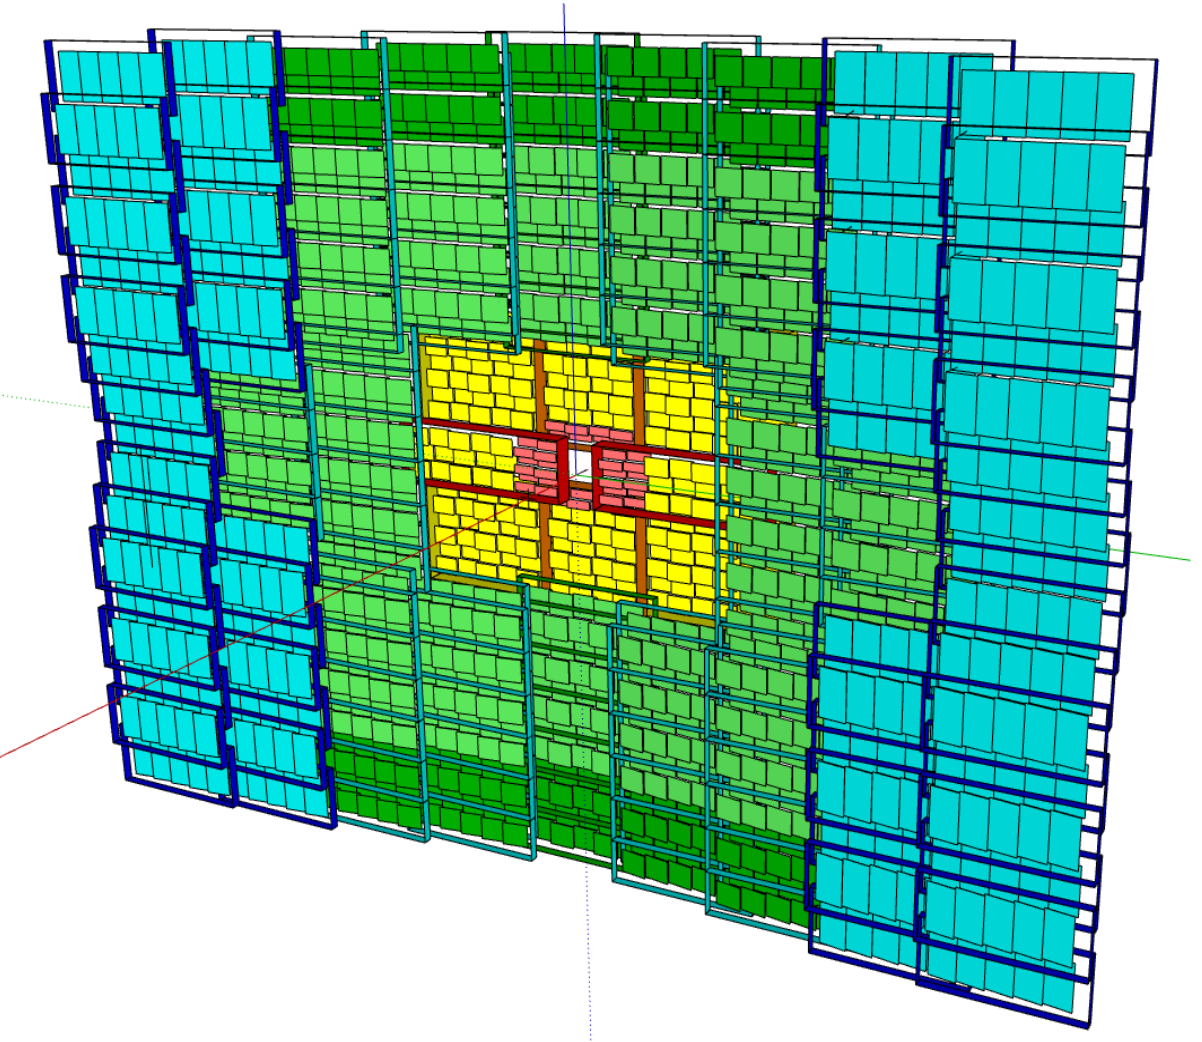
\includegraphics[width=1.0\textwidth]{pictures/TOF.png}
\caption{}
\label{fig:TOF}
\end{figure}

\subsubsection{Стартовый детектор SD}\label{sec:secSD}

Система для измерения времени пролёта возможна только при наличие детектора, регистрирующего момент старта --- временную отметку $T_{0}$ первичного взаимодействия.

%The proposal of a high performance TOF wall would be incomplete without the discussion of the time - zero (T 0 ) - reference that is needed for any velocity measurement. Details can be found in chapter 4 demonstrating that for all of the anticipated running scenarios solutions are available. For most of the heavy-ion reaction running at the initial SIS100 accelerator the software based T 0 - extraction is sufficient (see section 4.2). This method can be calibrated by making use of the diamond based start detector system developed for the HADES experiment (section 4.4) that is operational up to interaction rates of 100 kHz.

Высокочастотный стартовый детектор (Start Detector, SD), выполненный из алмаза и расположенный на пучке, может удовлетворить все требования CBM, включая полный диапазон пучка --- от протонов до тяжёлых ионов.
Такой детектор в то же время может эффективно использоваться для онлайн диагностики пучка, мгновенно выдавая информацию о профиле пучка, стабильности его положения по отношению к мишени, о количестве частиц в гало \todo и о временной структуре пучка.

%A high rate in-beam start detector (SD) could fulfill all CBM $T_{0}$ requirements, covering whole range of beams from proton to heavy-ions. Such detector is at the same time intended to be used for the on-line beam monitoring, giving the instantaneous information about the beam profile, the stability of the beam position on target, the amount of halo particles and time structure of the beam. In our opinion the best solution for such detector is an in-beam diamond Start detector.

SD будет расположен внутри вакуумной камеры. Его толщина должна быть минимальна, чтобы минимизриовать взаимодействие с пучком.

%SD will be installed inside the beam pipe in vacuum and it will measure the arrival time of every beam particle. In order to reduce the interactions in the SD itself its thickness has to be minimized. Fig. 4.4 shows the mounting of the planned SD system between the last focusing magnet in front of the cave and the focal point of the CBM detector.

% ==========================================================================================
% ==========================================================================================
% ==========================================================================================

\subsection{Электромагнитный калориметр ECAL}\label{sec:secECAL}

\begin{minipage}[t]{0.495\textwidth}
\begin{figure}[H]
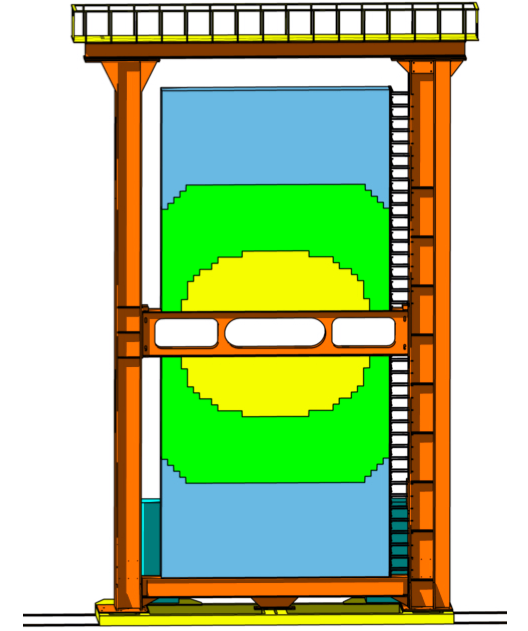
\includegraphics[width=0.95\textwidth]{pictures/CBM_ECAL_model.png}
\caption{Модель электромагнитного калориметра ECAL.}
\label{fig:ECAL}
\end{figure}
\end{minipage}
\begin{minipage}[t]{0.495\textwidth}
В эксперименте CBM будет установлен электромагнитный калориметр (Electromagnetic CALorimeter, ECAL) типа ``шашлык'', схожий с калориметрами экспериментов HERA-B, PHENIX и LHCb. Он будет использоваться для измерения прямых фотонов и нейтральных мезонов ($ \pi^{0}, \eta $), распадающихся на фотоны. Полный калориметр на SIS-300 будет собран из модулей, состоящих из 140 последовательных слоёв свинца и сцинтиллятора толщиной 1~мм. Планируется три типоразмера модулей: 3~см$\times$3~см, 6~см$\times$6~см и 12~см$\times$12~см. Модули могут быть организованы \\
%A ``shashlik'' type calorimeter as installed in the HERA-B, PHENIX and LHCb experiments will be used to measure direct photons and neutral mesons ($ \pi^{0}, \eta $) decaying into photons. The full ECAL at SIS-300 will be composed of modules which consist of 140 layers of 1 mm lead and 1 mm scintillator, with cell sizes of 3 cm$\times$3 cm, 6 cm$\times$6 cm and 12 cm$\times$12 cm. The shashlik modules can be arranged either as a wall or in a tower geometry with variable distance from the target. To simplify the detector layout and to fit in a very limited budget for ECAL at SIS100 stage we have reduced the number of ECAL sections considering only 4-cell modules.
Конфигурация для SIS-100 имеет 4352~канала считывания, составленные из 1088~модулей одного типа (6~см$\times$6~см). 
\end{minipage}

% ==========================================================================================
% ==========================================================================================
% ==========================================================================================

\subsection{Детектор непровзаимодействовавших осколков PSD}\label{sec:secPSD}

\todo \textbf{не провзаимодействовавших или непровзаимодействовавших} \todo

\todo
%Найти более новую картинку
\todo

\begin{minipage}[t]{0.495\textwidth}
\begin{figure}[H]
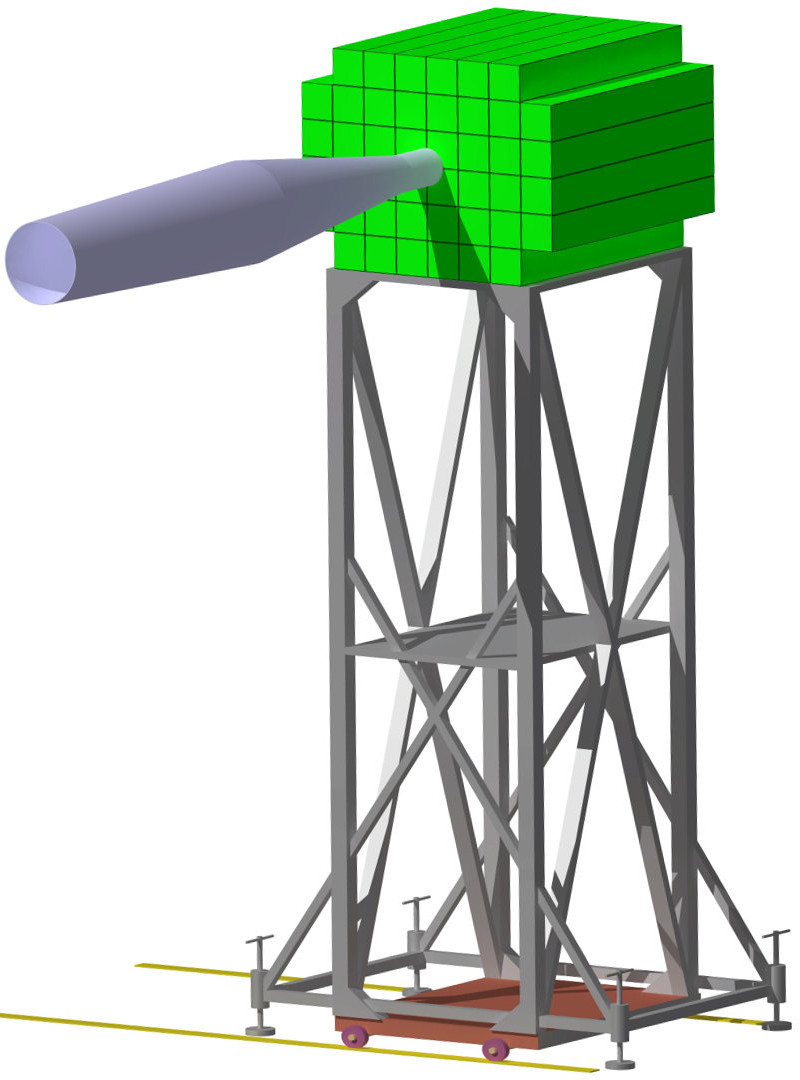
\includegraphics[width=0.95\textwidth]{pictures/CBM_PSD_model.png}
\caption{Модель калориметра PSD.}
\label{fig:PSD}
\end{figure}
\end{minipage}
\begin{minipage}[t]{0.495\textwidth}
Основная задача детектора непровзаимодействовавших осколков (Projectile Spectator Detector, PSD) --- выполнять измерения центральности столкновений тяжёлых ионов и ориентацию плоскости реакции. PSD представляет собой compensating \todo калориметр из свинца и сцинтиллятора, спроектированный для измерения распределения энергии налетающих осколков и летящих вперёд частиц, produced close to the beam rapidity.
Основные технические требования к PSD --- forward rapidity coverage и достаточное энергетическое разрешение для точного определения центральности столкновений, а также гранулярность в плоскости \todo, необходимая для восстановления плоскости симметрии столкновения. \\
%The main purpose of the PSD is to provide an experimental measurement of a heavy-ion collision centrality and orientation of its symmetry plane. The PSD is a compensating lead-scintillator calorimeter designed to measure the energy distribution of the projectile nuclei fragments (spectators) and forward going particles produced close to the beam rapidity.
%The main design requirements of the PSD are
%(i) forward rapidity coverage and sufficient energy resolution to allow for precise collision centrality determination and consequently of the number of participating nucleons and
%(ii) granularity in the plane transverse to the beam direction which is needed for the collision symmetry plane reconstruction.
\end{minipage}

Предлагаемый проект детектора, составленного из 44 модулей, покрывает широкий диапазон transverse area \todo вокруг области первичного взаимодействия так, чтобы большая часть непровзаимодействовавших фрагментов оставили всю свою энергию в PSD. За счёт вытянутой в горизонтальном направлении геометрии детектор PSD позволяет регистрировать фрагменты, отклонённые магнитным полем диполного магнита.
%The proposed 44 module design of the PSD covers large transverse area around the beam spot position such that most of the projectile spectator fragments deposit their energy in the PSD. The elongated transverse geometry of the PSD in horizontal direction takes into account the deflection of the fragments by the magnetic field of the CBM Dipole magnet.
%A lead-scintillator prototype of the PSD module with scintillator light readout by micropixel avalanche photodiodes and the PSD front-end electronics were tested with the proton and pion beams and cosmic muon rays. Radiation hardness and possible degradation of the PSD were studied with the FLUKA simulation of the CBM detector geometry.

В зависимости от энергии столкновения, PSD имеет разрешение по прицельному параметру, сравнимое с разрешением, предоставляемым кремниевой трековой системой STS. Таким образом, PSD предоставляет независимый метод в эксперименте CBM для определения центральности и множественности наблюдателей. В случае применения в связке с STS, детектор PSD помогает улучшить определение центральности 

%Depending on the collision energy, the PSD has a comparable impact parameter resolution to that of the CBM silicon tracking system (STS). Thus, the PSD provides an independent method in the CBM experiment of the centrality determination with spectator multiplicity. When used in a combination with the STS, the PSD helps to improve the overall centrality determination in the centrality range of 0--40\% and allows for centrality determination in narrow centrality classes with a width of at least 5\%.

Разрешение по определению плоскости реакции с помощью PSD варьируется в диапазоне от $\SI{30}{\degree}$ до $\SI{40}{\degree}$ в зависимости от расстояния \todo чего \todo от мишени и энергии столкновения. С учётом предлагаемой вытянутой геометрии детектора и после коррекции нелинейности детектора в азимутальном направлении, разрешение практически не меняется в зависимости от силы поля дипольного магнита CBM. Было проведено сравнение 

%The PSD event plane resolution varies in the range of 30--40 degrees depending on the distance from the target and the collision energy. With the proposed elongated geometry, and after correction for the detector azimuthal non-uniformity, the resolution of the PSD event plane shows negligible variation with the field strength of the CBM magnet. We compared the PSD event plane resolution with that of STS and an alternative detector setup at forward rapidity such as a forward time of flight (TOF) detector. We concluded that the PSD has significantly better event plane resolution than both STS and forward TOF detector configurations.


%%\subsection{Фундаментальные принципы черенковских детекторов}
%
%% Источник - http://nuclphys.sinp.msu.ru/enc/e186.htm
%
%\begin{minipage}[t]{0.495\textwidth}
%В основе черенковских детекторов лежит эффект Вавилова--Черенкова, который заключается в том, что заряженная частица испускает свет при движении в прозрачной среде со скоростью $\vartheta$ большей скорости света в этой среде, равной $c/n$, где $c$~---~скорость света в вакууме, а $n$~---~показатель преломления среды. Порог свечения: \\
%\begin{spacing}{1.5}
%{\centering
%$\beta = \frac{\vartheta}{c} \geq \frac{1}{n}$ \\}
%\end{spacing}
%Волновой фронт этого излучения представляет собой поверхность конуса, вершиной которого является частица, а осью --- её траектория. Угол раствора конуса $\theta$ фиксирован и определяется скоростью частицы $\vartheta$ и свойствами среды исходя из следующих соотношений: \\
%\begin{spacing}{1.5}
%{\centering
%$AC = \vartheta t = \frac{\vartheta c t}{c} = \beta c t$ \\
%$AB = \frac{c}{n} t$ \\
%$cos\theta = \frac{AB}{AC} = \frac{ct/n}{\beta c t} = \frac{1}{\beta n}$ \\}
%\end{spacing}
%\end{minipage}
%\begin{minipage}[t]{0.495\textwidth}
%\begin{figure}[H]
%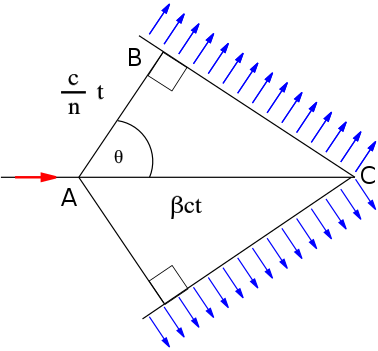
\includegraphics[width=0.9\textwidth]{pictures/Cherenkov.png}
%\caption{Геометрия черенковского излучения.}
%\label{fig:CherenkovGeo}
%\end{figure}
%\end{minipage}
%
%Черенковское излучение находится в области видимого света и ближнего ультрафиолета, что даёт возможность регистрировать его различными фотодетекторами.
%
%\subsubsection{-----------------------}
%
%За счёт того, что наличие свечения определяется скоростью, а не импульсом или энергией, связанными со скоростью через массу, предоставляется возможность идентификации частиц. При той же энергии более лёгкая частица будет иметь больше скорость, а более тяжёлая --- меньше скорость, причём возможно, что ниже порога свечения.
%Правильным подбором материала радиатора \todo ... выбирается диапазон энергий
%
%\subsection{Черенковские детекторы}
%
%% Источник - http://nuclphys.sinp.msu.ru/experiment/detectors/cherenk.htm
%
%Эффект Вавилова--Черенкова применяется в физике частиц для построения трёх типов детекторов: пороговых черенковских счётчиков, дифференциальных черенковских счётчиков \todo,\todo и черенковских детекторов кольцевого изображения (RICH-детекторов). 
%
%Пороговый черенковский счётчик служит для регистрации частицы, имеющей скорость выше порога свечения. Т.к. порог определяется материалом радиатора, существует возможность простейшей идентификации частиц путём установки двух или более различных радиаторов на пути пучка. Если, например, имеется два подобранных радиатора, то частицы одного типа будут светиться только в обоих, частицы другого типа --- только в одном, а третьи --- ни в одном.
%
%\begin{minipage}[t]{0.495\textwidth}
%\begin{figure}[H]
%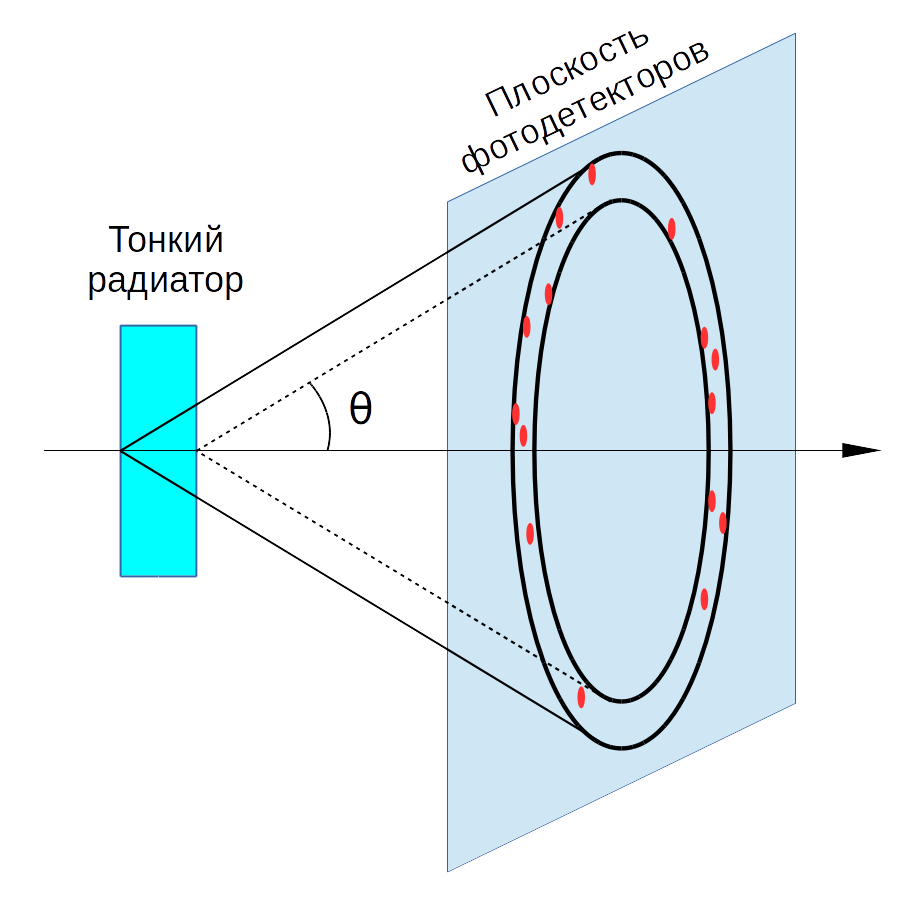
\includegraphics[width=0.9\textwidth]{pictures/RICH_scheme.png}
%\caption{Схема RICH-детектора \\с квазифокусировкой.}
%\label{fig:RICHbasic}
%\end{figure}
%\end{minipage}
%\begin{minipage}[t]{0.495\textwidth}
%\begin{figure}[H]
%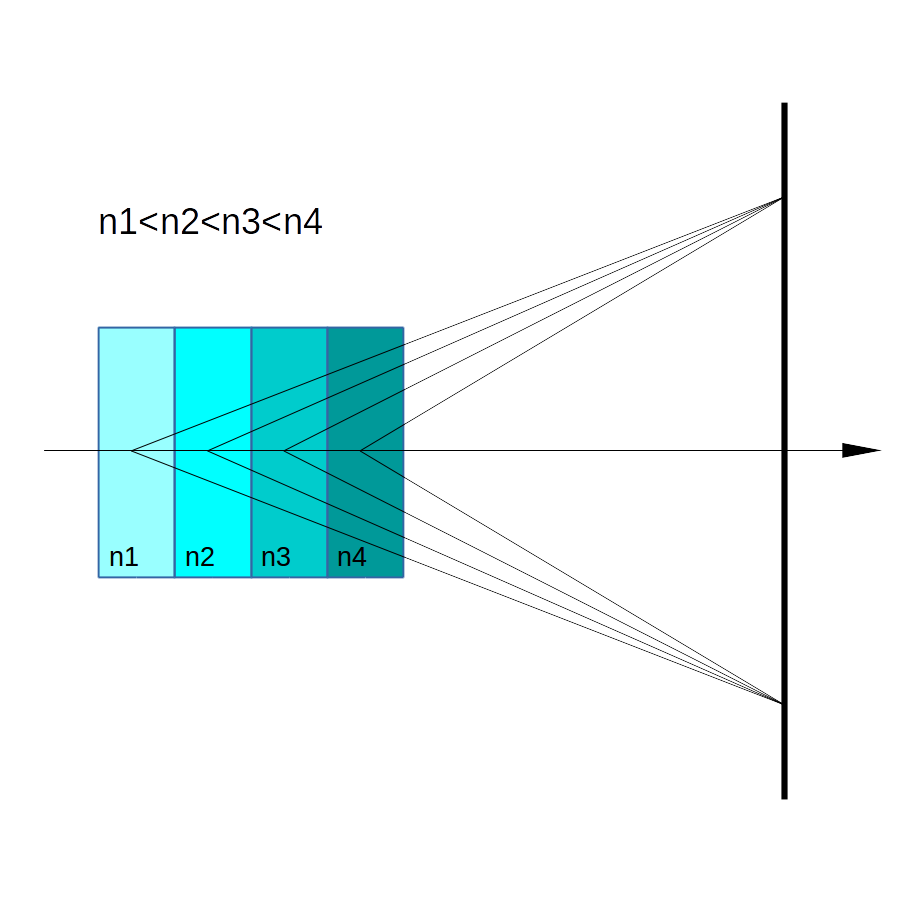
\includegraphics[width=0.9\textwidth]{pictures/RICH_layered.png}
%\caption{Схема RICH-детектора \\с многослойным радиатором.}
%\label{fig:RICHlayered}
%\end{figure}
%\end{minipage}
%
%Дифференциальные черенковские счетчики регистрируют частицы в определенном интервале скоростей. Т.к. черенковский угол пропорционален скорости, присутствует возможность построения оптической системы, разделяющей частицы, летящие под разными углами, то есть с разными скоростями. В зависимости от того, какая группа фоточувствительных элементов зарегистрировала свет, делается вывод о скорости пролетевшей частицы.
%
%RICH-детекторы используют тот факт, что черенковский свет излучается под постоянным углом $\theta$ к траектории частицы. Отсюда следует, что черенковский свет, возможно после оптической фокусировки, формирует изображение кольца в некоторой плоскости. RICH-детекторы можно классифицировать по нескольким признакам. По способу фокусировки RICH-детекторы можно разделить на три типа: с прямой фокусировкой, со сферическим или параболическим зеркалом и DIRC-детекторы.
%
%\textbf{Перетасовать!}
%(По радиатору:) В качестве радиатора может использоваться газ (самые распространённые --- $CO_{2}$, $CF_{4}$, $C_{4}F_{10}$), жидкий или твёрдый материал, как частный случай --- аэрогель.
%(По фотодетектору:) Микроканальные пластины, ФЭУ, фотодиоды, ...
%\textbf{Перетасовать!}
%
%Если поставить на пути черенковского света плоскость фотодетекторов, то, с учётом того, что радиатор имеет конечную длину, на ней образуется изображение кольца. На~\figref{fig:RICHbasic} показана схема RICH-детектора с квазифокусировкой (прямой фокусировкой), в которой радиатор обычно выбирается тонким и с большим показателем преломления. Это позволяет регистрировать кольцевое изображение напрямую, без какой-либо дополнительной оптической подсистемы. Для того чтобы преодолеть проблему малого выхода фотонов в небольшом объёме радиатора применяют слоистые радиаторы (см.~\figref{fig:RICHlayered}), в которых каждый следующий слой имеет больший показатель преломления, и следовательно, больший угол черенковского света.
%
%Во втором варианте RICH-детекторов оптический материал радиатора одновременно используется и как черенковский радиатор, и как светопровод (см.~\figref{fig:DIRC}). Радиатор (например кварц) имеет прямоугольную форму. За счет этого, фотоны черенковского излучения, испущенные под углом $\theta$, распространяются вдоль пластины за счет полного внутреннего отражения с сохранением этого угла до самого торца пластины, где расположен позиционно-чувствительный фотоприёмник. Такой тип детекторов называют DIRC-детекторами (Detection of Internally Reflected Cherenkov light).
%
%\begin{figure}[H]
%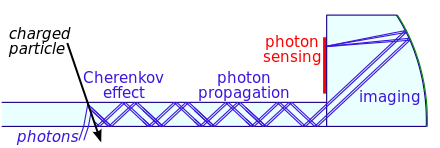
\includegraphics[width=0.7\textwidth]{pictures/DIRC.png}
%\caption{Принцип DIRC-детекторов.}
%\label{fig:DIRC}
%\end{figure}
%
%\begin{minipage}[t]{0.495\textwidth}
%\begin{figure}[H]
%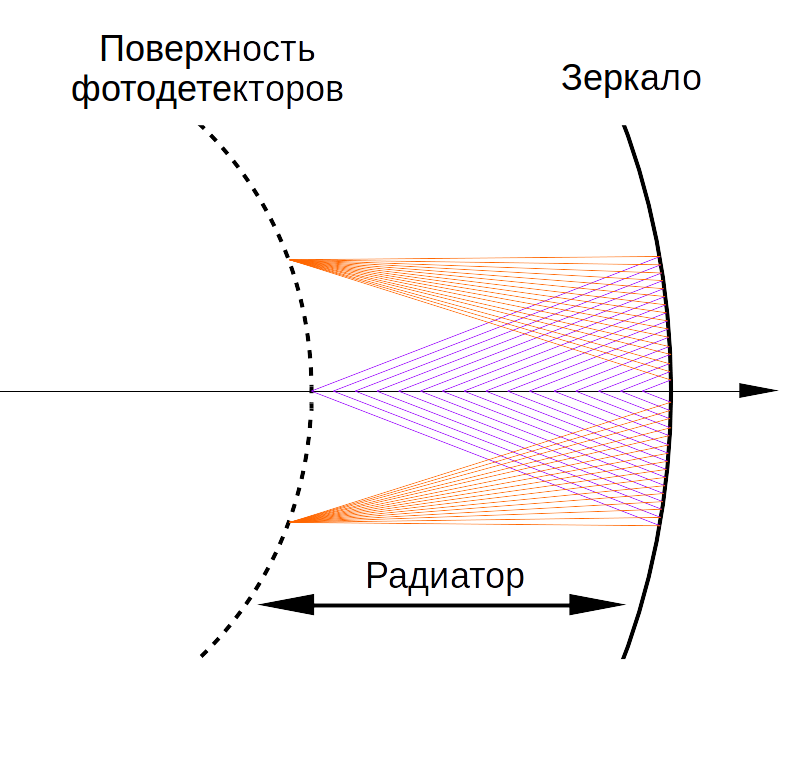
\includegraphics[width=0.9\textwidth]{pictures/RICH_spherical.png}
%\caption{Схема RICH-детектора \\со сферическим зеркалом.}
%\label{fig:RICHspherical}
%\end{figure}
%\end{minipage}
%\begin{minipage}[t]{0.495\textwidth}
%Если в качестве радиатора используется газ, для того чтобы излучалось достаточное количество фотонов, толщина радиатора должна быть довольно большой. В этом случае для фокусировки используются сферические или параболические зеркала. В таком детекторе радиатор находится между двумя сферическими поверхностями (см.~\figref{fig:RICHspherical}). Наружная --- сферическое зеркало радиуса $R$. Источник частиц находится в центре сферы. На внутренней сфере радиуса $R/2$ устанавливаются фотодетекторы. Отраженное от зеркала черенковское излучение фокусируется на внутреннюю сферу, образуя кольцо радиусом $r = R/2 \times tg(\theta)$. Для того чтобы вывести фотодетекторы из аксептанса детектора зеркало может быть повёрнуто, а иногда применяют и дополнительные плоские зеркала (см. \todo). Из конструктивных соображений поверхность фотодетекторов нередко выполняют плоской или собирают из нескольких плоских модулей.
%Так, например, в CBM RICH используются оба упомянутых приёма --- фокусная цилиндрическая поверхность аппроксимируется набором плоских модулей МА~ФЭУ, расположенных за пределом аксептанса детектора, а фокусировка выполняется одним отражением от сферических зеркал, размещённых в стороне от пучка и повёрнутых на некоторый угол.
%\end{minipage}

\section{RICH-детектор эксперимента CBM}

%\todo \textbf{Может как-то сделать так, чтобы это описание CBM рича было после описания других ричей --- COMPASS, LHCb, HERA-b? Или как раз наоборот, лучше сразу после этой секции?}

%\todo \textbf{Перенести какую-то часть из секции RICHgeom}

По той причине, что в столкновении тяжёлых ионов рождается огромное количество заряженных $\pi$-мезонов, возникает необходимость идентифицировать электроны и позитроны.

Детектор черенковских колец (Ring Imaging CHerenkov detector, RICH) решает задачу идентификации частиц в диапазоне импульсов от до 8~\GeVoverC{}.
В паре с детектором переходного излучения TRD, покрывающем более высокие импульсы, RICH позволяет идентифицировать сигнальные электроны от лёгких векторных мезонов и $J/\psi$.

Фактор подавления пионов $\pi_{suppr}$ определяется как отношение количества восстановленных в STS треков, имеющих продолжение в геометрическом аксептансе детектора RICH, к количеству пионов, идентифицированных как электроны.

Для получения дилептонных спектров на SIS300 требуется $\pi_{suppr}$ порядка 10000, что осуществимо при совместном применении TRD и RICH, причём $\pi_{suppr}$ последнего должен составлять как минимум 100.

В случае SIS100 фон обусловлен такими источниками как $\gamma$-конверсия в мишени или распад $\pi^{0} \rightarrow \gamma + e^{+} + e^{-}$.



% Из диссера Копфера

%For SIS100 the background is already dominated by physical sources like $\gamma$-conversion in the target or $\pi^{0}$-Dalitz decays at a pion suppression factor of $10^3$ (see section 2.6). The electron identification covers the full angular acceptance of the CBM detector, i.e. from \SI{2.5}{\degree} to \SI{25}{\degree} in polar angle and full azimuthal coverage. In order to accommodate the bending of tracks in the dipole magnet, all detectors behind the magnetic field will be wider by a factor 1.5 compared to the height.


CBM RICH имеет $CO_{2}$ радиатор, который характеризуется коэффициентом преломления $n=1.00045$ при $T=0$ и $p=1$ атм.



%\todo остаётся?
%Порог черенковского свечения для пионов составляет $p=4.65$~\GeVoverC.

CBM RICH предсталяет собой классический RICH-детектор с газовым радиатором, с одним сферическим зеркалом и МА~ФЭУ в качестве фотодетекторов.


Аксептанс детектора, с учётом расширения по горизонтали из-за наличия магнитного поля, разводящего частицы, представляет собой конус \SI{0}{\degree}--\SI{25}{\degree} с вершиной в точке первичного взаимодействия, растянутый по горизонтали в 1.5 раза. Таким образом в плоскости XY угол составляет \SI{0}{\degree}--\SI{37.5}{\degree}.
% Перенесено из RICHgeom
Аксептанс детектора составляет $\SI{25}{\degree}$ по вертикали и $\SI{37.5}{\degree}$ по горизонтали. Длина отведённого под детектор пространства вдоль оси пучка составляет 1900~мм, при этом передняя плоскость находится на расстоянии 1800~мм от точки взаимодействия, а задняя, соответственно, на расстоянии 3700~мм. Ещё 100~мм перед RICH отводится под пространство для стыковки магнита, STS, RICH и пучковой трубы. Исходя из того факта, что зеркала должны полностью покрывать геометрический аксептанс, ширина детектора выбрана 5268~мм, а высота 4420~мм.

% Перенесено из RICHgeom
\begin{figure}[H]
\centering
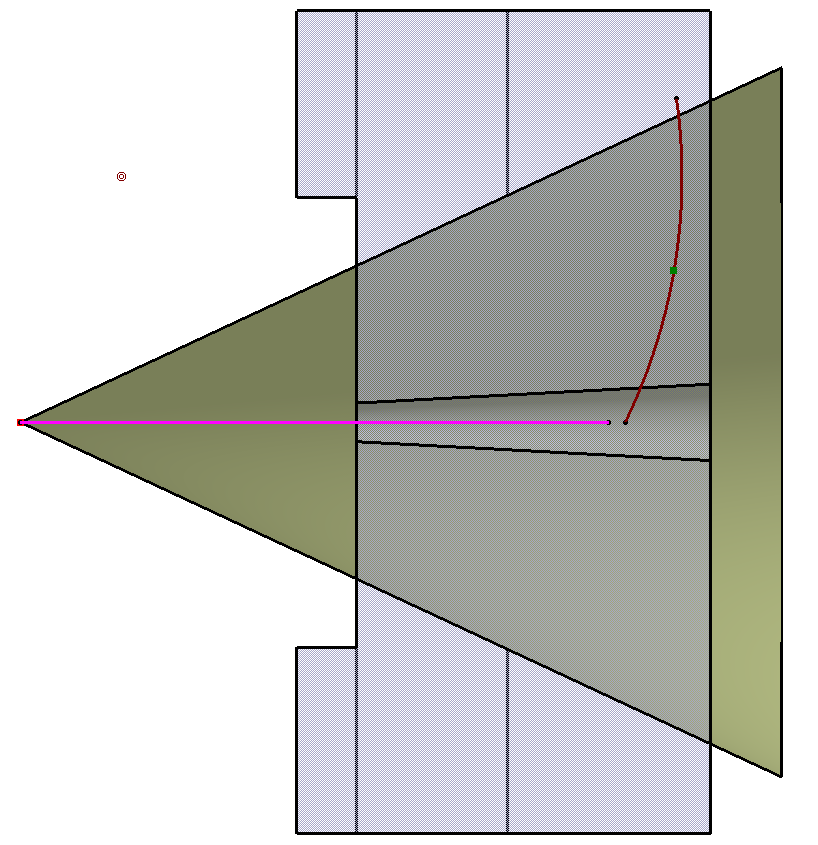
\includegraphics[width=0.7\textwidth]{pictures/RICH_construction.png}
\caption{Схема детектора CBM RICH, сид сбоку. Жёлтый конус -- геометрический аксептанс.}
\label{fig:RICHconstruction}
\end{figure}

% Перенесено из RICHgeom
На раннем этапе проектирования CBM RICH исходя из доступного пространства в общей экспериментальной установке было рассчитано, что фокусирующая система CBM RICH должна выполнять одно отражение с помощью двух сферических зеркал радиусом 3~метра, расположенных на расстоянии 3500~мм от точки взаимодействия. Рассматривался также вариант с двойным отражением, при этом вторая группа зеркал была плоская. Зеркала расположены симметрично относительно горизонтальной плоскости, проходящей через ось пучка, и полностью покрывают аксептанс детектора. Площадь каждого зеркала составляет приблизительно 7.5~м$^2$.

% Перенесено из RICHgeom
Для того чтобы выполнить требование к точности, зеркало такого радиуса технологически возможно изготовить только из сегментов. Рассматривались варианты изготовления различными компаниями, прототипы исследовались на \todo D0, Ronchi test, в итоге остановились на \todo.
Сегмент зеркала будет иметь размер около 40см$\times$40см. (точное значение указать невозможно, это ж не прямоугольник)

\subsection{Радиатор}

Разделение электронов и пионов в диапазоне импульсов до 10~\GeVoverC{} требует низкого коэффициента преломления радиатора, что определяет выбор углекислого газа в качестве радиатора. $CO_{2}$ имеет пороговый гамма-фактор $\gamma _{th} = 1 / \sqrt{1 - 1/n^{2}} = 33.3$, где $n = 1.00045$ --- коэффициент преломления при температуре $\SI{0}{\degreeCelsius}$, давлении 1000~мбар и длине волны 600~нм. Порог черенковского излучения для заряженных пионов составляет $p = 4.65$~\GeVoverC, а для электронов и позитронов --- $p = 0.03$~\GeVoverC. При этом порог для каонов $\approx 16$~\GeVoverC. \todo saturated черенковский угол для ультрарелятивистских частиц равен $\SI{1.72}{\degree}$. Полагая, что пионы и электроны могут быть разделены с эффективностью до 90\% \todo при максимальном черенковском угле $\theta = arccos(1/n)$, верхняя граница по импульсу при радиаторе из $CO_{2}$ получается $\approx$ 10~\GeVoverC.

% The separation of electrons and pions at momenta below 10~\GeVoverC requires a low refractive index of the radiator and therefore determines the radiator to be a gas. A $CO_{2}$ radiator is foreseen which has a threshold Lorentz factor of $\gamma _{th} = 1 / \sqrt{1 - 1/n^{2}} = 33.3$, given a refractive index of $n = 1.00045$ at a temperature of \SI{0}{\degreeCelsius}, a pressure of 1000~mbar, and a wavelength of 600~nm. The Cherenkov threshold is $p = 4.65$~\GeVoverC for charged pions and $p = 0.03$~\GeVoverC for electrons and positrons. The threshold for kaons is $\approx 16$~\GeVoverC. The saturated Cherenkov angle for ultrarelativistic particles is $\SI{1.72}{\degree}$. Assuming that pions can be separated from electrons up to 90\% of the maximum Cherenkov opening angle $\theta = arccos(1/n)$, electrons and pions can be separated up to $\approx$ 10~\GeVoverC with $CO_{2}$ as radiator gas.

Размер RICH-детектора определяется доступным пространством между кремниевой трековой станцией STS, расположенной внутри магнита, и детектором переходного излучения TRD. С одной стороны, высокая длина радиатора предпочтителька, т.к. она определяет высокий выход черенковских фотонов. С другой стороны чем меньше расстояние между последней станцией STS и первой станцией TRD, тем выше эффективность трекинга. Из этих соображений для RICH отведено пространство от 1800~мм до 3700~мм по оси пучка, не ограниченное по другим осям ничем, кроме пола. Перед RICH и за ним отведено ещё по 100~мм общего пространства для стыковки с STS и TRD. Зеркало расположено на расстоянии 3500~мм от точки взаимодействия, таким образом, рабочая длина радиатора составляет 1700~мм.

% The radiator length is 1.7~m and the volume $\approx 35 m^{3}$. Since the RICH detector will be placed between the STS in the dipole magnet and the TRD detector, its overall length is constrained by the distance between the magnet and its shielding yokes at about 1.6~m from target and the first TRD station. On the one hand, a long radiator is favourable due to the proportionality between photon yield and radiator length according to equation (2.8). On the other hand, a short gap between the tracking detectors STS and TRD is advantageous for tracking which requires a short RICH detector in between. In consequence, the overall length of the RICH detector including radiator, mirror, and support structure is foreseen to be $\approx 2$~m.

Нижняя граница длин волн при выборе радиатора определяется нижней границей длин волн чувствительности фотодетекторов

When designing a RICH detector ``one has to be extremely careful in matching the choice of (gas-)radiator with the sensitive wavelength range of the photon detection system'' [66]. In the case of the CBM-RICH, the low wavelength limit of the photomultiplier sensitivity (see section 3.4) coincides well with the absorption edge of $CO_{2}$ at $\approx 185$ nm (see section 6.2.1).

Явление chromatic absorption в $CO_{2}$ становится заметным только в области длин волн менее 200~нм и, следовательно, не ухудшает разрешения черенковского кольца.

%For $CO_{2}$, chromatic absorption becomes sizeable only in the region below 200 nm (see section 6.2.1) and does not deteriorate the Cherenkov ring resolution significantly as shown below.

Т.к. $CO_{2}$ не показывает высокого уровня сцинтилляции его часто добавляют в радиаторы, где другой газ является основным, в качестве гасящего газа. Ожидается около 5~фотонов/МэВ, в основном в синей области спектра. Энерговыделение в радиаторе порядка 1~\GeV ожидается при центральном $Au+Au$ столкновении, где рождается $\approx 1000$ минимально ионизирующих частиц, приводящих к $\approx 5000$ сцинтилляционных фотонов, летящих изотропно вдоль трека частицы. Если консервативно предположить, что 20\% фотонов достигает плоскости фотодетекторов и 25\% из них регистрируется, то в результате данного эффекта регистрируется дополнительно около $250$ фотонов, распределённых равномерно. При общем числе каналов порядка 55~000, указанный шум от сцинтилляции добавляет до 0.45\% \todo по всем каналам. Данный показатель находится в допустимом пределе и CBM RICH не теряет в эффективности.

%Due to the fact that $CO_{2}$ does not exhibit a high level of scintillation, it is often added to other radiator gases as quenching gas. Approximately 5 photons/MeV, mostly in the blue wavelength range, are expected [69]. An energy deposit in the radiator of $\approx 1$ GeV is expected for a central Au+Au collision with $\approx 1000$ minimum ionizing particles [6] leading to 5000 scintillation photons emitted isotropically along the particle tracks. This leads to $\approx 250$ measured additional photons distributed homogeneously over the photon detector plane when conservatively assuming that 20\% of the photons reach the photon camera with 25\% of them being detected. Given the total of 55 000 channels, noise from scintillation will add up to 0.45\% of all channels. This is well within the noise level that the CBM-RICH detector can tolerate without performance loss [6].

\subsection{Система фокусировки}

%The mirror of the CBM-RICH detector is split into two parts above and below the beam pipe. Each mirror half is oriented towards a photon detection plane and part of a sphere with R = 3.00 m. The total area of the two mirror halves is $12.96 m^2$ . The mirror halves consist of 36 mirror tiles each arranged in four rows of nine tiles. The tiles themselves have a slightly trapezoidal shape in order to minimise gaps in between to 3~mm to~4 mm. Two different tile sizes are foreseen, 430/425.6 mm $\times$ 425~mm for the inner two rows and 425.5/412.5~mm $\times$ 425~mm for the outer rows.

%The mirror tiles are made of a 6~mm thick SIMAX glass substrate front-coated with $Al+MgF_{2}$. Aluminium provides a good reflectivity in both the visible and the UV wavelength region down to below 200~nm. The $MgF_{2}$ layer is used as protective layer in order to prevent the formation of UV absorbing aluminium oxide. Mirror tiles from JLO Olomuc were successfully tested in a prototype (see section 5.1), characterised in terms of homogeneity [70] and reflectivity [71], and chosen to be used for the CBM-RICH detector.

%A tripod concept is foreseen for mounting the mirror tiles on an aluminum frame. Each mirror tile is glued to three actuators allowing for the precise alignment of the tiles in a sphere.

%In order to reduce the production of secondary particles, the material budget of the RICH detector has to be kept low. The mirror support structure is therefore designed as a compromise between stability and light weight.

% Перенесено из RICHgeom
В CBM RICH каждый сегмент зеркал будет крепиться на раме с помощью трёх \todo моторизированных актуаторов с удалённым управлением. Это позволяет корректировать положение отдельных сегментов 



\subsection{Фотодетекторы}

Задача фоточувствительной камеры CBM RICH --- детектировать черенковские фотоны, рождённые заряженными частицами в радиаторе и отражённые от зеркала. Камера разрабатывается для регистрации одиночных фотонов с высокой эффективностью. Для эффективного выполнения реконструкции необходима точная регистрация координат и времени прилёта каждого фотона.

%Task of the CBM-RICH photon camera is the detection of Cherenkov photons produced by charged particles in the gas radiator and reflected by the focusing mirror. The camera is developed for the detection of single photons with high efficiency. A precise measurement of position and time of arrival of each photon is required as input for the ring reconstruction algorithm discussed in section 2.5.3.

Фоточувствительная камера CBM RICH состоит из двух половин, расположенных над и под пучком в фокальной плоскости сферических зеркал. Обе половины находятся рядом с дипольным магнитом

%The photon camera of the CBM-RICH detector consists of two parts, one above and one below the beam pipe in the focal plane of the spherical mirrors. The two photon detector planes are located in front of the CBM dipole magnet shielded by the magnet yokes. The Cherenkov rings from the upper mirror half will be projected onto the upper photon detector, rings from the lower mirror half onto the lower photon detector. Each of the two photon detector planes is divided into two parts in order to optimise the angle towards the mirror. Thus, the camera consists of four separated areas, so-called camera modules. Each module covers an area of 0.6~m $\times$ 1.0~m (height $\times$ width). The total active camera area is $2.4 m^{2}$ .

%The CBM-RICH design foresees the usage of commercially available multianode photomultiplier tubes (MAPMTs) as photon sensors. The use of Micro Channel Plate (MCP) sensors is considered as alternative [6]. Due to the good geometrical coverage of these sensor types, no focusing elements like lenses or Winston cones are envisaged.

\subsection{Магнитное поле в области фоточувствительной камеры}

Моделирование распределения магнитного поля, созданного дипольным магнитом, с помошью пакета TOSCA показало, что фоточувствительная камера расположена в области, где паразитное поле составляет 10--50~мТл. Измерения показали, что для планируемой модели МА~ФЭУ эффективность регистрации одиночных фотонов значительно падает, если поле превышает уровень 1--2~мТл. Таким образом, магнитное поле в области фотосенсоров должно быть опущено до допустимого уровня.

% According to TOSCA 3 calculations, the photon camera is exposed to significant magnetic stray fields in the order of 10~mT to 50~mT. Measurements show that the single photon detection efficiency of the foreseen MAPMTs drops significantly for values exceeding 1~mT to 2~mT especially in the edge and corner pixels [6]. Therefore, the magnetic field strength in the region of the photon sensors has to be kept below this value.

Есть два способа уменьшить поле в области камеры --- повернуть зеркало и, следовательно, отодвинуть камеру от магнита, и поставить магнитный экран вокруг камеры. В CBM RICH была проведена оптимизация угла наклона зеркала точки зрения эффективности реконструкции и было решено спроектировать магнитный экран вокруг камеры.
Есть также третий вариант, который заключается во введении дополнительного отражения на пути черенковских фотонов. Этот подход, однако, был исключён, т.к. дополнительное отражение приводит к увеличению необходимой светочувствительной плоскости, а это значительно увеличивает стоимость детектора.

%In order to cope with the magnetic stray field in the region of the photon camera, two design options are considered and currently studied. The first option is to rotate the two mirror planes and to move the camera modules further away from the beam axis where the magnetic stray field is lower. In addition, a shielding box enfolding the camera modules can reduce the magnetic field strength in the region of the photocathodes significantly. The second option is the use of a second mirror reflecting the Cherenkov photons to the camera positioned farther away from the magnet. This option, however, requires a larger camera surface due to an increased focal length. Details on all design options can be found in [6].


%Ссылка на прогресс репорт 2015 стр. 53.

% Перенесено из RICHgeom
Положение фоточувствительной камеры в пространстве определяется относительно зеркал исходя из соображений эффективности регистрации колец. В CBM детектор RICH расположен непосредственно за дипольным магнитом, причём отражённые от сферических зеркал черенковские фотоны летят в направлении противоположном пучку. Уменьшение угла наклона зеркал теоретически приводит к повышению эффективности детектора, но на практике невозможно из-за нехватки пространства для размещения камеры в небольшом зазоре между магнитом и конусом аксептанса RICH. Увеличение угла наклона зеркал позволило бы вывести фотодетектор далее вверх из области магнитного поля, но это приводит к нежелательным оптическим эффектам, отрицательно влияющим на эффективность. Следовательно, камера должна быть расположена очень близко к дипольному магниту. Отсюда возникает необходимость экранировать камеру от магнитного поля, составляющего 50-100~мТл в области МА~ФЭУ. Рассчитано, что данное семейство МА~ФЭУ может работать в магнитном поле до 1~мТл без снижения эффективности.

\subsection{Характеристики детектора}

Ниже представлены результаты моделирования в среде CbmRoot в связке с генератором UrQMD, выполненные (\todo не мной!) с применением актуальной геометрической модели CBM RICH, построенной с помощью ``CATIA-GDML geometry builder'' и описанной в секции~\ref{sec:chapRICHgeo}.
Результаты показывают прирост по всем показателям по сравнению с геометрией, в которой каждая фоточувствительная камера моделируется двумя плоскостями, что даёт основание полагать, что цилиндрическая форма камеры более эффективна.

В CBM RICH выработано два типовых анализа модели детектора с помощью МК моделирования. В первом анализе в геометрической установке присутствует только RICH и он обстреливается одиночными электронами из точки первичного взаимодействия с импульсом и направлением из заданного диапазона. Такой анализ позволяет оценить выход черенковских фотонов, количество регистрируемых фотонов (хитов) (см.~\figref{fig:RICHchar1}), геометрический аксептанс детектора, а также параметры восстановленных колец.

Реконструкция колец в RICH состоит из двух этапов --- поиск колец, т.е. группировка хитов, принадлежащих одному кольцу (ring finding), и фитирование, т.е. определение параметров кольца (ring fitting), причём фитирование выполняется и окружностями и эллипсами.
МК моделирование позволяет не выполнять первый этап так, как это делалось бы на реальных данных, а принять за хиты одного кольца список хитов от фотонов, рождённых от рассматриваемого электрона (\todo parentID).
При этом второй этап индифферентен к истории хитов.
На~\figref{fig:RICHchar2} представлены распределения радиуса $R$ подобранного кольца, полуосей $A$ и $B$ подобранного эллипса. На~\figref{fig:RICHchar3} показаны распределения разброса хитов от кольца $dR$ и эллиптичности $B/A$.
Следует отметить, что в алгоритме поиска колец значение 7 выбрано как минимально допустимое количество хитов в кольце.
В случае МК моделирования с одиночными электронами возможна ситуация, когда количество хитов в кольце меньше~7 (см.~\figref{fig:RICHchar1} (справа)). Это означает, что такое кольцо теоретически есть, но не будет восстановлено. \todo формулировка

\begin{figure}[H]
\begin{minipage}[t]{0.495\textwidth}
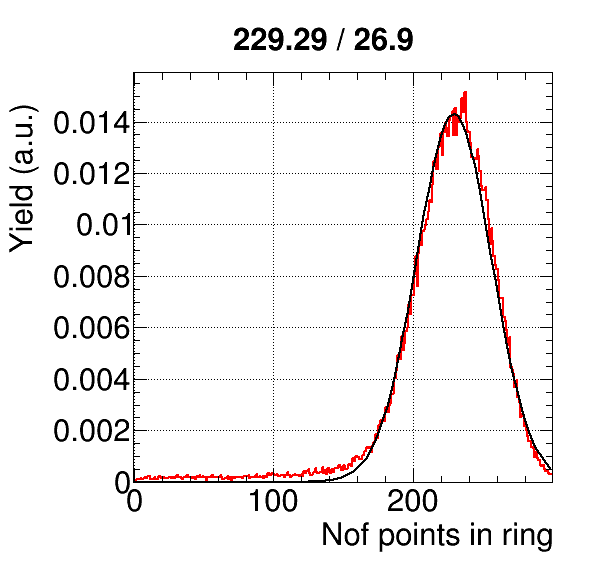
\includegraphics[width=0.9\textwidth]{pictures/RICH_nPoints_dist.png}
\end{minipage}
\begin{minipage}[t]{0.495\textwidth}
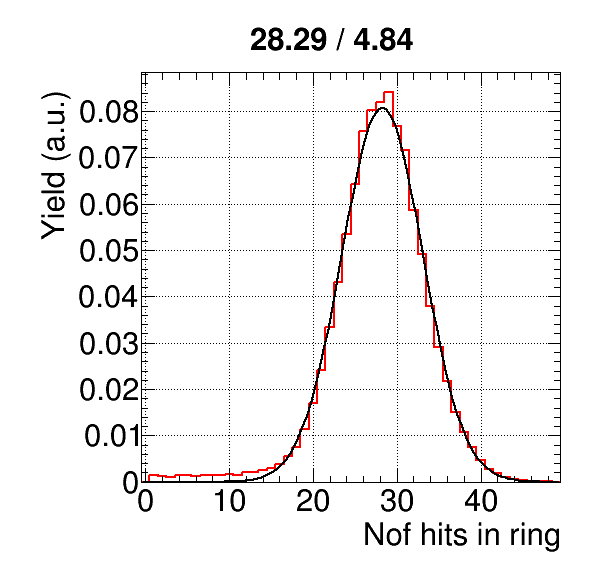
\includegraphics[width=0.9\textwidth]{pictures/RICH_nHits_dist.png}
\end{minipage}
\caption{}
\label{fig:RICHchar1}
\end{figure}

\begin{figure}[H]
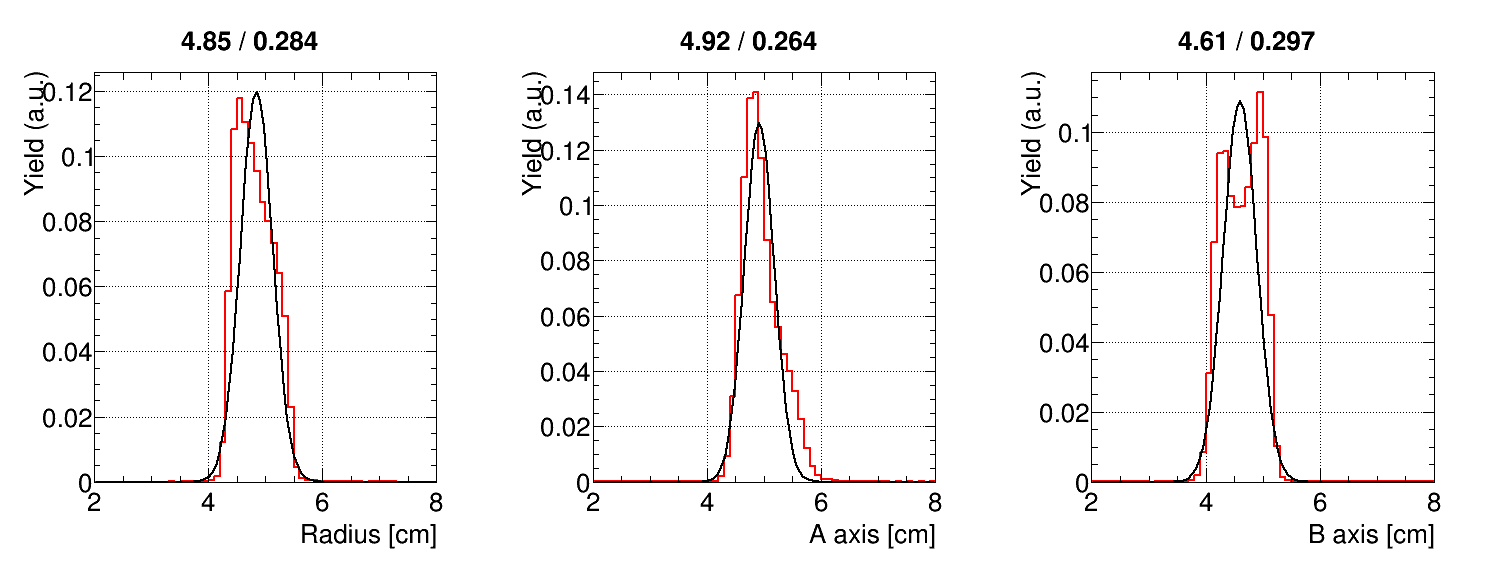
\includegraphics[width=0.95\textwidth]{pictures/RICH_R_A_B.png}
\caption{}
\label{fig:RICHchar2}
\end{figure}

\begin{figure}[H]
\begin{minipage}[t]{0.495\textwidth}
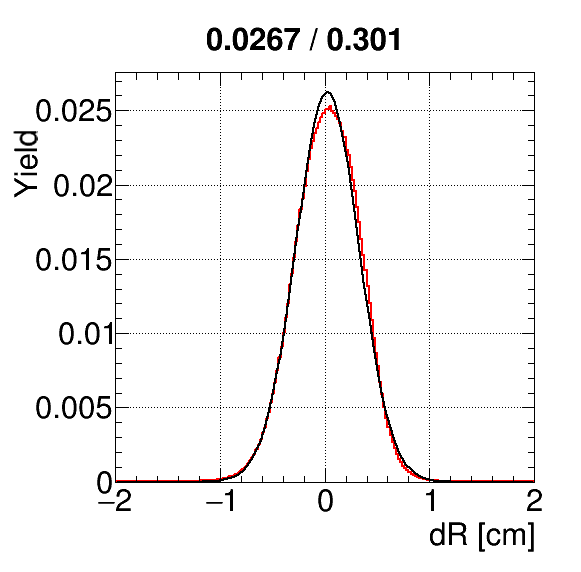
\includegraphics[width=0.9\textwidth]{pictures/RICH_dR.png}
\end{minipage}
\begin{minipage}[t]{0.495\textwidth}
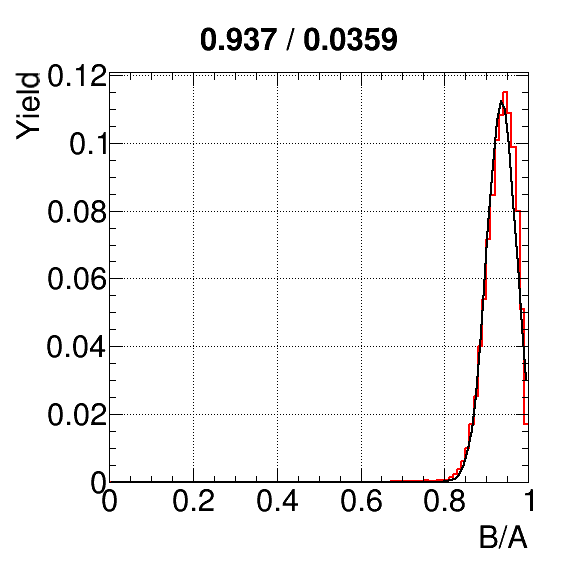
\includegraphics[width=0.9\textwidth]{pictures/RICH_BoverA.png}
\end{minipage}
\caption{}
\label{fig:RICHchar3}
\end{figure}

%Все значения - средние.
%Один электрон рождает 230 фотонов, из которых регистрируется 28 фотонов.
%Радиус кольца 4.85~см, отношение полуосей эллипсов $A/B=$0.937.


Второй анализ выполняется по результатам моделирования стандартного $Au+Au$ события CBM с помощью UrQMD. В этом случае есть две группы событий --- центральные столкновения при энергии 8~\GeVperNucl{}, характерные для SIS100, и 25~\GeVperNucl{}, характерные для SIS300.

Т.к. задача данного моделирования --- оценить функционирование детектора в реалистичной ситуации, в геометрической установке присутствуют STS и магнит. При этом присутствует магнитное поле и выполняется полная реконструкция треков в STS. На~\figref{fig:CbmRichOneEvent} представлено изображение на одной плоскости реконструкции от одного события $Au+Au$ 25~\GeVperNucl{}. Красные точки обозначают хиты, зелёные --- пересечение с плоскостью реконструкции RICH продолжений восстановленных треков STS, отражённых от зеркала.

\begin{figure}[H]
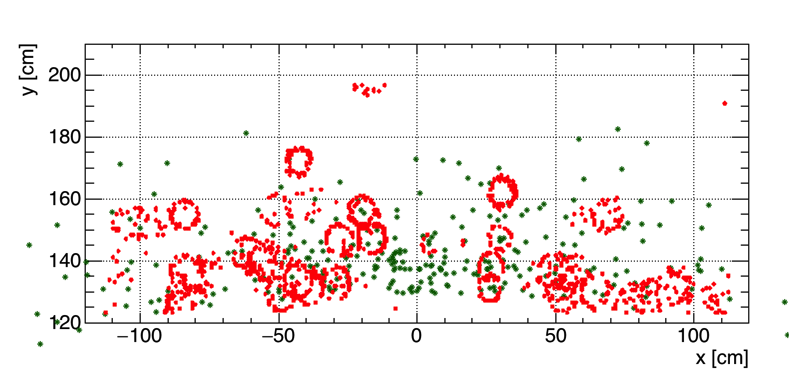
\includegraphics[width=0.9\textwidth]{pictures/CbmRichOneEvent.png}
\caption{Типовое событие (UrQMD, 25~\GeVperNucl{}) в одной фотодетектирующей плоскости RICH. Красные точки --- хиты RICH, зелёные --- продолжения треков STS.}
\label{fig:CbmRichOneEvent}
\end{figure}


\begin{table}[H]
\caption{}
\label{tabl:RICHAuAuChar}
\begin{tabular}{ | p{0.3\linewidth} | p{0.3\linewidth} | p{0.3\linewidth} | }
\hline
& 8~\GeVperNucl{} (SIS100) & 25~\GeVperNucl{} (SIS100) \\
\hline
$N_{hits}$ & 496 & 1431 \\
\hline
$N_{rings}$ ($\geq1$~хита) & 23.0 & 71.6 \\
\hline
$N_{rings}$ ($\geq7$~хитов) & 19.9 & 59.6 \\
\hline
\end{tabular}
\end{table}

\begin{figure}[H]
\begin{minipage}[t]{0.495\textwidth}
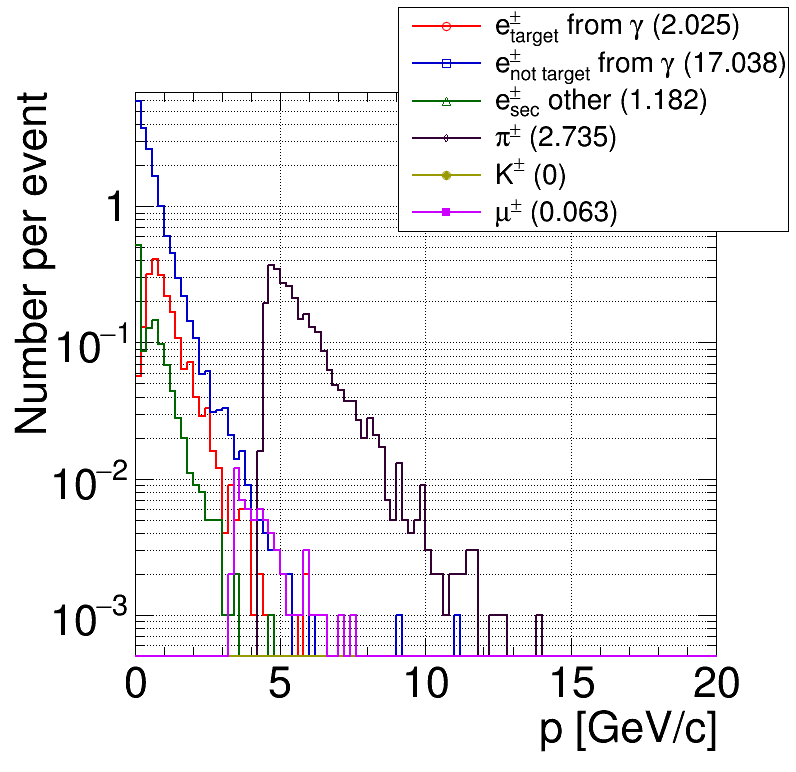
\includegraphics[width=0.9\textwidth]{pictures/RICH_8AGeV.png}
\end{minipage}
\begin{minipage}[t]{0.495\textwidth}
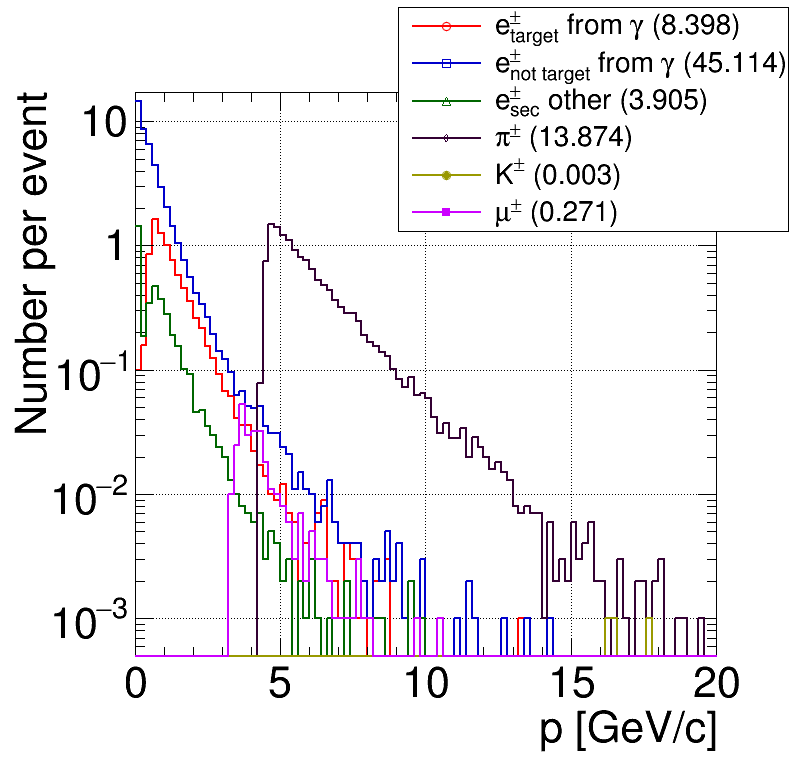
\includegraphics[width=0.9\textwidth]{pictures/RICH_25AGeV.png}
\end{minipage}
\caption{Основные типы частиц, регистрируемые в RICH при центральном $Au+Au$ столкновении при~8~\GeVperNucl{} (слева) и~25~\GeVperNucl{} (справа).}
\label{fig:RICH8and25AGeV}
\end{figure}



\section{Обзор существующих детекторов черенковских колец}\label{sec:secRiches}

%По-видимому второй рич так и остался в планах...
\subsection{COMPASS RICH-1}\label{sec:CompassRich1}

%\subsection{COMPASS}\label{sec:Compass}

% Википедия
% https://en.wikipedia.org/wiki/COMPASS_experiment

Экспериментальная установка NA58, также известная как COMPASS (``Common Muon and Proton Apparatus for Structure and Spectroscopy'') представляет собой систему из двух спектрометров длиной 60~метров за неподвижной мишенью на отводе пучка M2 ускорителя SPS в CERN. Эксперимент был предложен в 1996 году, в период с 1999 по 2001 года выполнялись работы по установке и в 2001 был выполнен первый (commissioning) запуск. Набор данных разбит на два этапа: COMPASS I (2002--2011) и COMPASS II (2012--2018). 

% http://link.springer.com/article/10.1140/epjst/e2008-00800-2

%\subsubsection{COMPASS RICH-1}\label{sec:CompassRich1}

% Самое свежее (2014) - http://compassweb.ts.infn.it/rich1/paper/tessarotto_instr14.pdf

% Ссылки
% NIM A 02 (2003) 112–116
% doi:10.1016/S0168-9002(02)02165-4
% E. Albrecht et al.
% https://wwwcompass.cern.ch/compass/detector/rich/publications/NIMA502-112.pdf

% http://wwwcompass.cern.ch/compass/proposal/pdf/proposal.pdf

% https://pub.uni-bielefeld.de/download/2301233/2301236
% 8.2.2 The Mirror Wall

Детектор Черенковских колец \mbox{RICH-1} был спроектирован в 1996~г. и функционирует с 2002~г. \mbox{RICH-1} подвергается постоянной оптиимизации, а в 2006~было выполнено обновление. Ожидается второе обновление детектора в 2016~г. \todo оно было?

Основная задача детектора Черенковских колец --- разделение $\pi$, $p$ и $K$ в диапазоне импульсов от 3~до~55~ГэВ/с в условиях высокой интенсивности (что бы это значило\todo в статье 2014 г. написано, что beam rate 40 МГц, и частота триггеров 20 кГц) в полном аксептансе спектрометра, составляющем $\pm$250~мрад по горизонтали и $\pm$180~мрад по вертикали. Для минимизации отрицательного влияния на эффективность стоящих ниже по пучку электромагнитного и адронного калориметров детектор \mbox{RICH-1} должен иметь минимум количества материала в аксептансе. Также в процессе проектирования COMPASS \mbox{RICH-1} необходимо было развивать технологии для реализации возможности регистрировать и справляться с высоким для того времени потоком данных.
\todo \textbf{По большому счёту, задачи те же, что и у CBM}

Габариты корпуса детектора COMPASS \mbox{RICH-1}, выполненного из алюминия, составляют 6.6$\times$5.3$\times$3.3~м$^3$. Внутри расположен газовый радиатор $C_{4}F_{10}$ длиной 3~м и объёмом около 83~м$^3$. Пороги по импульсу для Черенковского света: для $\pi$ --- 2.5~ГэВ/с, для $K$ --- 8.9~ГэВ/с и 17~ГэВ/с для $p$. В центре детектора проходит цилиндрический ионопровод диаметром 100~мм, наполненный гелием.
% The original beam pipe, made of 150 mm thick stainless steel, has been replaced in 2012 by a lighter pipe, made of 4 layers of metalized BoPET (25mm BoPET + 0.2mm Al): the contribution to the total material budget by the new pipe for beam particles is 0.08\% X0 (plus 0.06\% due to helium).
Газовая система закрытого типа поддерживает радиатор под избыточным давление $100\pm10$~Па.

Система фокусировки состоит из двух сферических зеркал радиусом 6.6~м, составленных из 116~сегментов шести- и пятиугольной формы, общей площадью более 21~м$^2$. Для фокусировки на фоточувствительные камеры, расположенные за пределами геометрического аксептанса, центры сфер зеркал смещены по вертикали от пучка на 1.6~м, а образовавшийся в результате этого зазор между двумя зеркалами приводит к потере 4\% площади отражающей поверхности. Зеркала были произведены компанией IMMA, Ltd., Kinskeho 703, Turnov, Czech Republic.
Коллаборацией COMPASS был разработан метод контроля индивидуальных отклонений сегментов зеркал ``на лету'' (онлайн), называемый CLAM (``a continuous line alignment and monitoring method'').

\todo \textbf{картинка - схема, оч похоже на CBM}

Исходя из необходимости иметь суммарную площадь фоточувствительных камер 5.3~м$^2$, изначально для реализации были выбраны многопроволочные пропорциональные камеры (MWPC) с сегментированным фотокатодом из CsI. \mbox{RICH-1} оборудован восемью идентичными камерами, каждая площадью 576$\times$1152~мм$^2$. Фотокатоды выполнены из двух двухсторонних печатных плат размером 576$\times$576~мм$^2$. Окна из silica-quartz состоят из двух одинаковых quartz-plates размером 600$\times$600$\times$5~мм$^3$. Сегментированный фотокатод обеспечивает размер пикселя 8$\times$8~мм$^2$ и в общей сложности 82944 канала.

% Ещё подробности тут: http://localhost/Lib/Long_term_experience_and_performance_of_COMPASS_RI.pdf

В 2006~г. с целью повышения эффективности детектора было выполнено комплексное обновление центральной области фоточувствительной камеры, составляющей 25\% от всей площади. MWPC были заменены на МА~ФЭУ с индивидуальными линзами и соответствующей считывающей электроникой. В общей сложности было установлено 4 панели по 144~МА~ФЭУ Hamamatsu R7600-03-M16, имеющими 16~каналов и входное стекло, прозрачное в ультрафиолетовой области, и специальный делитель напряжения.

% For the physics runs starting in 2016 COMPASS RICH-1 will be equipped with new MPGD-based photon detectors, which have been developed by a dedicated R&D program.

Сигнал с МА~ФЭУ считывается платами передней электроники, основанными на ASIC ``CMAD'', реализующем 8-канальный предусилитель-дискриминатор, разработанный на основе ``MAD4'' специально для COMPASS \mbox{RICH-1}. CMAD позволяет работать на частоте до 5~МГц на канал.

%The signals from the MAPMTs are read by a fast digital electronics system [36, 37] based on the 8 channels CMAD [38] preamplifier-discriminator, developed for COMPASS RICH-1 as an upgraded version in CMOS technology of the MAD4 [39] front-end chip. The CMAD has a small noise level (1 fC), the possibility to set individual channel thresholds, a good time resolution and high rate capability: it provides full efficiency up to an input rate of 5 MHz per channel. The design of the front-end boards and the optimization of the thresholds setting allows to completely suppress the MAPMTs cross talk signals while keeping the single photoelectron detection efficiency at a 95\% level.

\todo \textbf{перефразировать}
Хорошее временное разрешение МА~ФЭУ не портится за счёт использования цифровых карт DREISAM, в которых реализован ВЦП F1, имеющий временное разрешение 110~пс и может работать с чатотой до 10~МГц на канал и частоте триггера до 100~кГц.

%The good MAPMT time resolution is fully exploited with the help of digital cards, called DREISAM, housing the dead-time free F1 TDC [40] , which has a time resolution of 110 ps and can stably operate up to 10 MHz per channel input rate and 100 kHz trigger rate.

Считывающая электроника COMPASS \mbox{RICH-1} монтируется на детектор, образуя очень компактную установку, которая экранирована от внешнего электромагнитного поля медными пластинами, выполняющими также и роль радиаторов, охлаждаемых водой циркуирующей по медным трубкам.

%All the electronics components of the RICH-1 readout system are directly mounted on the detector and form a very compact setup. Each PCB is coupled to a copper plate providing both efficient electromagnetic shielding and good cooling power: thermalized water circulates in underpressure condition in thin copper pipes brazed onto the copper plates [36]. The stability and uniformity of the water cooling system has been achieved after several improvements of the distribution system and of the operation and maintenance protocols.

Оцифрованные данные с плат передней электроники передаются по оптике платам считывания CATCH, которые группируют данные и передают дальше также по оптике через S-LINK в систему сбора данных эксперимента.

%Data from the front-end cards are transferred via optical links to a set of CATCH readout-driver modules which concentrate the data and send them via S-LINK transmitter and optical fibre to the COMPASS DAQ system.

%Expected occupancy level is $\approx$5\% at a maximum trigger rate of $10^5 s^{-1}$, resulting in a maximum data flow of 2.5 GB/s. COMPASS-Gassiplex chips are used as front-end-chips. These are modified versions of the chips developed for RD26, now equipped with preamplifier, shaper and an analog-multiplexer. The intrinsic dead time is 400 nsec per event, with a peaking time of 1 usec. The value for noise is as low as 1100 electrons equivalent at a gas amplification of $\approx$6.5 mV / (fC).

%The core piece of the readout system is the total amount of 192 front-end-cards, the 60 cm long BORA boards [67], hosting the front-end chips and a first trigger level. There are 24 BORA-boards per photon chamber handling 432 analog channels. Each single BORA-board is equipped with front-end-chips, ADCs (analog digital converter), FIFOs (first in first out buffer), FPGAs (field programmable gate array) of the type VIRTEX XCV100 [68] for logic sequencers, threshold-subtraction and zero-suppression, 32-bit DSPs [69] for event packaging, on-board controls and optical links. The event processing time is 10usec. The control system for those BORA-boards is a parallel network of DSPs (digital signal processing), operated via a dedicated PC-PCI-interface: the DOLINA-boards with 8 on-board DSPs each. To avoid grounding interference between the PC and the detector all BORA-boards are optoisolated from DOLINA with the help of specific optoisolating boards. Figure 8.11 sketches the architecture of the readout system. The photon detectors reach an absolute gain of 10 4 at nominal voltage of 2000 V with photon detection efficiencies of about 75\% as presented in Figure 8.12.

\textbf{Заключение такое, что в целом конструкция этого RICH очень схожа с конструкцией CBM RICH.}

%\subsubsection{COMPASS RICH-2}\label{sec:CompassRich2}

\subsection{LHCb}\label{sec:LHCb}

% http://localhost/Lib/10.1.1.668.3561.pdf - An Overview of the Status of the LHCb RICH Detectors - 2008

\todo \textbf{ПРОСТО ЦЕЛИКОМ ПЕРЕВЕСТИ СЕКЦИЮ 2.1 ОТСЮДА:}
%http://localhost/Lib/art_10.1140_epjc_s10052-013-2431-9.pdf
Performance of the LHCb RICH detector at the LHC - 2013




LHCb is one of the four major experiments at the LHC, and is dedicated to the study of CP violation and the rare decay of heavy flavours. It is a forward spectrometer designed to accept forward-going b- and c-hadrons produced in proton-proton collisions. The layout of the spectrometer is shown in \figref{fig:LHCb}

\begin{figure}[H]
\centering
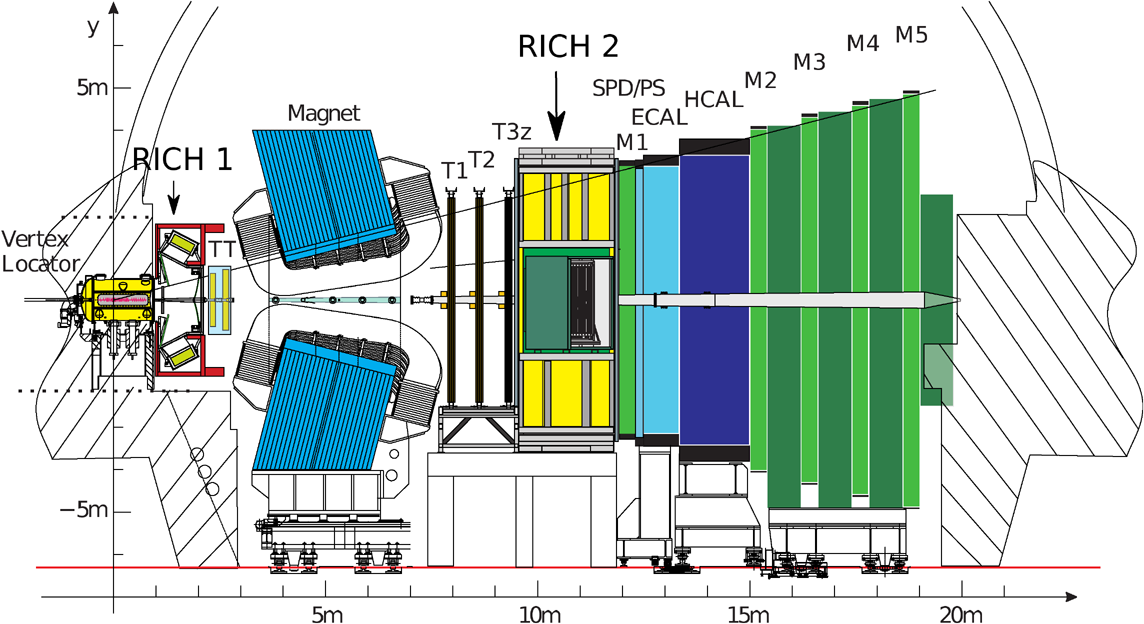
\includegraphics[width=1.0\textwidth]{pictures/LHCb.png}
\caption{Схема установки LHCb.}
\label{fig:LHCb}
\end{figure}

PID from 2 to 100~\GeVoverC
Два рича полностью охватывают необходимый угловой аксептанс 15–300 mrad with respect to the beam axis.


RICH1 covers the low and intermediate momentum region 2–40~\GeVoverC over the full spectrometer angular acceptance of 25–300 mrad. The acceptance is limited at low angle by the size of the beampipe upstream of the magnet. RICH2 covers the high-momentum region 15–100~\GeVoverC, over the angular range 15–120 mrad.

RICH1 is placed as close as possible to the interaction region. To minimize the material budget there is no separate entrance window, and the RICH1 gas enclosure is sealed directly to the exit window of the VELO vacuum tank. The downstream exit window is constructed from a low-mass carbon-fibre/foam sandwich.

RICH2 is placed downstream of the magnet, since the high momentum tracks it measures are less affected by the magnetic field. In this way it can be placed after the downstream tracking system in order to reduce material for the measurement of the charged tracks. The entrance and exit windows are again a foam sandwich construction and skinned with carbon-fibre and aluminium, respectively.

Both RICH detectors have a similar optical system, with
a tilted spherical focusing primary mirror, and a secondary
flat mirror to limit the length of the detectors along the beam
direction. Each optical system is divided into two halves on
either  side  of  the  beam  pipe,  with  RICH 1  being  divided
vertically and RICH 2 horizontally. The vertical division of
RICH 1 was necessitated by the requirements of magnetic
shielding for the photon detectors, due to their close prox-
imity to the magnet. The spherical mirrors of RICH 1 (4 seg-
ments) are constructed in four quadrants, with carbon-fibre
structure, while those of RICH 2 (56 segments), and all flat
mirrors  (16  and  40  segments  in  RICH 1  and  RICH 2  re-
spectively), are tiled from smaller mirror elements, employ-
ing a thin glass substrate.


Fluorocarbon gases at room temperature and pressure are
used as Cherenkov radiators; C4F10 in RICH 1 and CF4 in
RICH 2 were chosen for their low dispersion. The refractive
index is respectively 1.0014 and 1.0005 at 0 C, 101.325 kPa
and 400 nm. About 5\% CO2 has been added to the CF4 in
order to quench scintillation in this gas.

The momentum threshold for kaons to produce Cherenkov
light in C4F10 is 9.3 GeV/c. Particles below this momentum
would only be identified as kaons rather than pions in veto
mode, i.e. by the lack of Cherenkov light associated to the
particle. To maintain positive identification at low momen-
tum and in order to separate kaons from protons, a second
radiator is included in RICH 1: a 50 mm thick wall made of
16 tiles of silica aerogel [10] at the entrance to RICH 1. The
refractive index is n=1.03 and the light scattering length is
around 50 mm at 400 nm in pure N2. The aerogel is placed
in the C4F10 gas volume and a thin glass filter is used on the
downstream face to limit the chromatic dispersion.

...

\subsection{HERA-b RICH}\label{sec:HerabRich}

% http://localhost/Lib/rich-instr99-nim453.pdf
% 0303012.pdf - The HERA-B Ring Imaging Cerenkov Counter

Эксперимент HERA-b \todo \textbf{пару слов}. Схема экспериментальной установки представлена на \figref{fig:HERAbSetup}.

HERA-B, a fixed target experiment (see Fig. 1) at the HERA storage ring at DESY, was designed [1] to measure rare processes in the decays of B mesons. The B mesons are produced in collisions of 920 GeV/c protons with a fixed target, which consists of 8 wires which can be individually inserted into the halo of the proton beam in order not to disturb experiments measuring ep collisions. One of the essential components of the spectrometer is the Ring Imaging Cherenkov counter (RICH) [1,2,3,4]. The main purpose of the RICH counter is the identification of charged hadrons, in particular kaons from decays of B mesons. Identifying charged kaons essentially means separating them from pions in the momentum range between 3 GeV/c and about 50 GeV/c at an interaction rate of up to 40 MHz.

\begin{figure}[H]
\centering
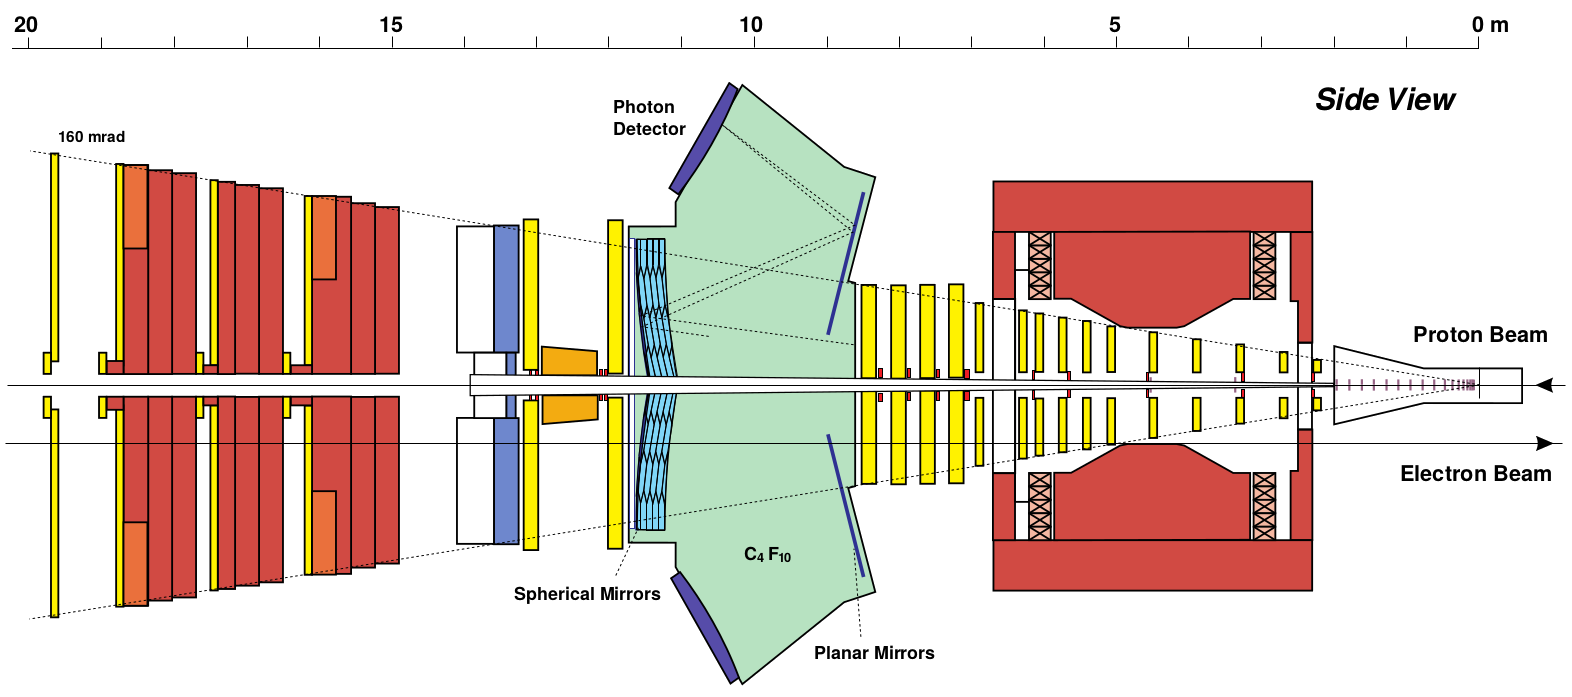
\includegraphics[width=1.0\textwidth]{pictures/HERA_b_setup.png}
\caption{Схема установки HERA-b.}
\label{fig:HERAbSetup}
\end{figure}

Схема детектора RICH эксперимента HERA-b показана на \figref{fig:HERAbRICH}. Он имеет газовый радиатор $C_{4}F_{10}$ объёмом 108~м$^3$ и массой 1100~кг. Длина радиатора 2.8~м, коэффициент преломления n=1.00137, порог импульса для рождения Черенковских фотонов для пионов и каонов составляет 2.7~\GeVoverC и 9.6~\GeVoverC соответственно. Для частиц с $\beta=1$ Черенковский угол равен 51.5~мрад (52.4~мрад), а разница между пионами и каонами составляет 0.9~мрад при 50~\GeVoverC. Радиатор поддерживается при избыточном давлении 2.5~мбар.

Корпус детектора изготовлен из нержавеющей стали, кроме передней и задней стенок из алюминия толщиной 1~мм. После фокусировки фотоны выходят из корпуса через стенку толщиной 2~мм из оргстекла прозрачного в ультрафиолетовой области. Передняя стенка HERA-b RICH расположена на расстоянии 8.5~м от мишени.

Система фокусировки состоит из двух пар зеркал, расположенных симметрично относительно горизонтальной плоскости, проходящей через ось пучка. Первое зеркало сферическое, второе --- плоское. Сферические зеркала (см. \figref{fig:HERAbRICHmirrors}) составлены из 80 полных или обрезанных шестиугольных сегментов, имеют радиус 11.4~м и толщину 7~мм. Они покрывают прямоугольную область 6$\times$4~м, общая площадь 24~м$^2$. Каждый сегмент крепится к раме трёмя моторизированными актуаторами с удалённым управлением. Для фокусировки за пределы геометрического аксептанса сферические зеркала наклонены на 9$^\circ$ от пучка. Каждое из двух плоских зеркал состоит из 18 сегментов.

HERA-b RICH имеет две фоточувствительные камеры, расположенные соответственно над и под пучком. Одна фоточувствительная камера (см. \figref{fig:HERAbRICHcamera}) составлена из 7 супермодулей 1.1$\times$0.4~м$^2$. Поверхность камеры аппроксимирует эллиптический цилиндр. Один супермодуль состоит из $16 \times 6$ модулей, каждый экранирован от магнитного поля тонкими пластинами из soft iron. В общей сложности было установлено 1488 МА~ФЭУ R5900-00-M16 и 752 МА~ФЭУ R5900-03-M4 фирмы Hamamatsu т.е 26816 каналов. Габариты одного такого МА~ФЭУ составляют 28$\times$28~мм$^2$, а чувствительная площадь 18$\times$18~мм$^2$. Перед каждым МА~ФЭУ стоят две линзы для того, чтобы привести в соответствие площадь, занимаемую МА~ФЭУ, и чувствительную. Использование линз приводит к тому что размер пикселя становется равным $9 \times 9$~мм$^2$ у 16-пиксельного R5900-00-M16 и $18 \times 18$~мм$^2$ e 4-пиксельного R5900-03-M4.
МА~ФЭУ монтируются на платы-адаптеры $70 \times 70$~мм$^2$, на которых осуществляется распределение высокого напряжения и аттенюация сигнала с МА~ФЭУ. Платы передней электроники построены на основе чипа ASD8 --- предусилителя, формирователя и дискриминатора. Сигналы с передней электроники передаются по 16-канальному кабелю типа витая пара длиной 7.5~м к драйверам передней электроники (front end dirver, FED). 1~FED имеет 4~дочерние платы, к каждой подключено 16~кабелей, и одну материнскую. 1~FED обрабатывает 1024 канала, всего используется 28 таких наборов. Материнская плата выполняет роль интерфейса к DAQ системе всегй установки HERA-b и имеет буфер, в котором может храниться до 128 событий в ожидании сигнала от триггера первого уровня.

%33 хита на частицу с $\beta=1$.

\begin{figure}[H]
\begin{minipage}[b]{0.45\textwidth}
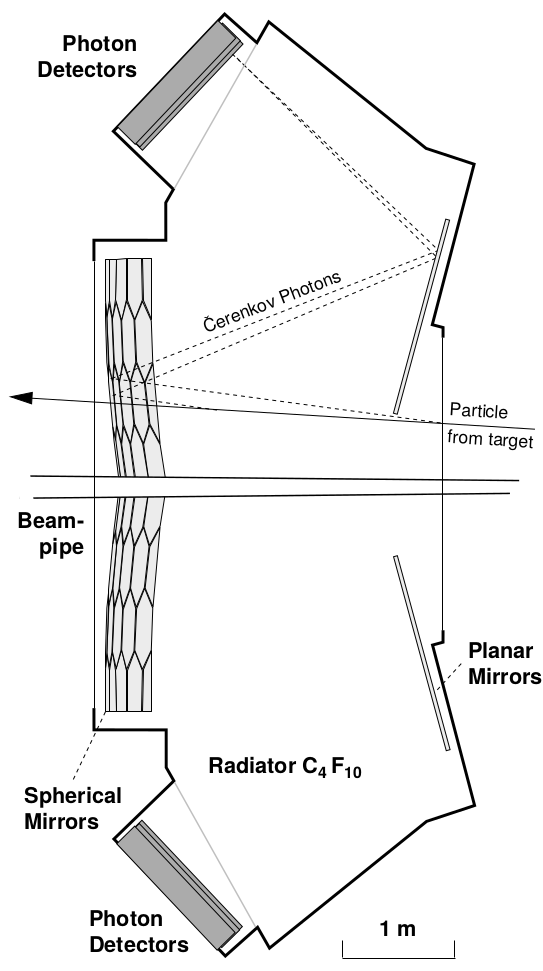
\includegraphics[width=0.9\textwidth]{pictures/HERAb_RICH.png}
\caption{Схема детектора HERA-b RICH.}
\label{fig:HERAbRICH}
\end{minipage}
\hspace{0.01\textwidth}
\begin{minipage}[b]{0.545\textwidth}
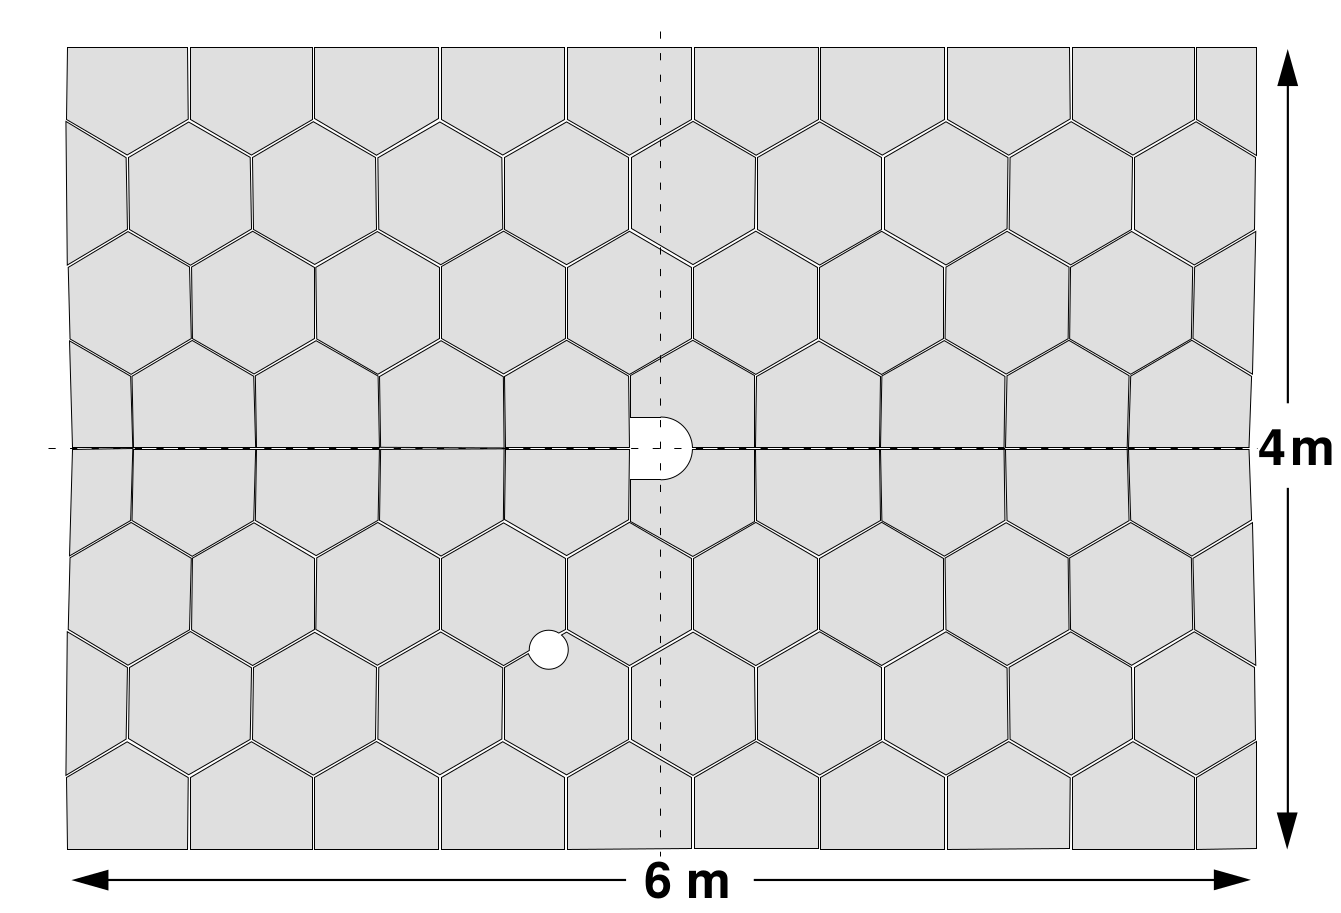
\includegraphics[width=1.0\textwidth]{pictures/HERAb_RICH_mirrors.png}
\caption{Схема компоновки сферических зеркал HERA-b RICH.}
\label{fig:HERAbRICHmirrors}
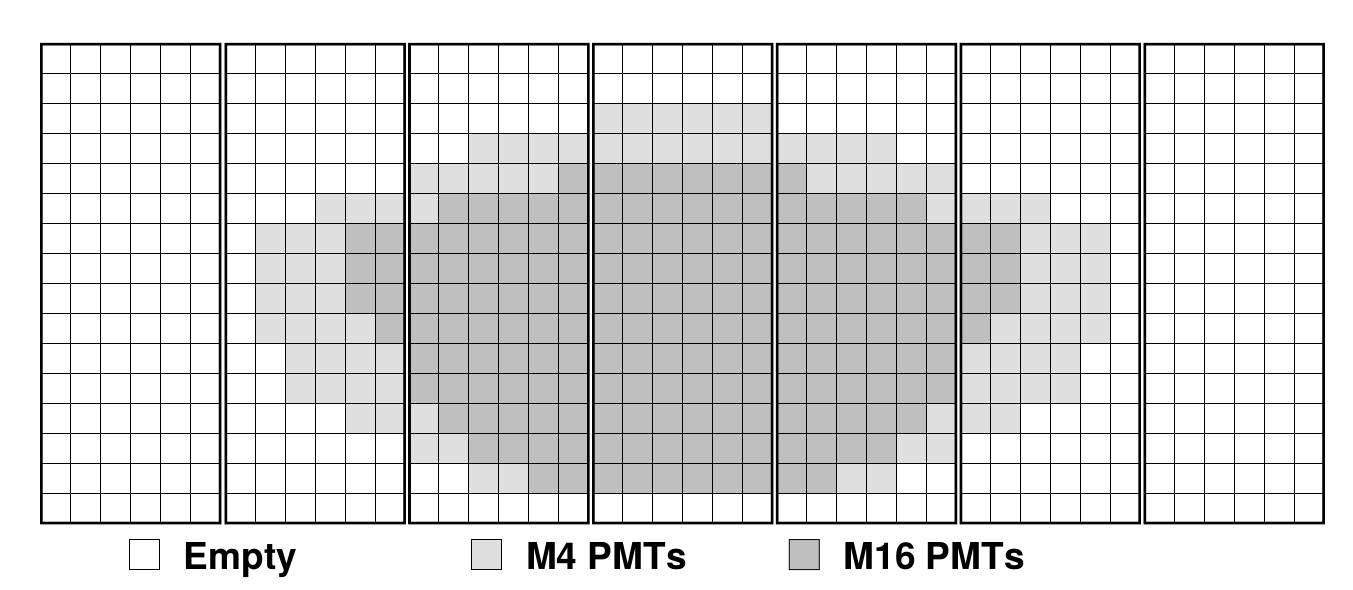
\includegraphics[width=1.0\textwidth]{pictures/HERAb_camera.png}
\caption{Схема заполненности одной фоточувствительной камеры HERA-b RICH. Одна ячейка соответствует модулю из 8~МА~ФЭУ.}
\label{fig:HERAbRICHcamera}
\end{minipage}
\end{figure}


\section{Обработка сигнала с детектора}\label{sec:secSignalProcessing}

Экспериментальная установка в физике высоких энергий или физике тяжёлых ионов ставит своей задачей восстанавливать события, произошедшие в области первичного взаимодействия. Такой областью будет являться точка взаимодействия пучка с мишенью в случае эксперимента с фиксированной мишенью, либо точка взаимодействия встречных пучков на коллайдерном эксперименте. Для выполнения этой задачи в некоторой области рядом с точкой взаимодействия ставят набор из нескольких детекторов, регистрирующих вторичные частицы и их продукты распада. Детекторы вырабатывают электрические сигналы, которые в случае современного крупного эксперимента необходимо доставить в ЭВМ, чтобы выполнять программную обработку, включающую в себя реконструкцию треков и частиц и анализ многочисленных распределений.

%В зависимости от исследуемой физики, детекторы могут охватывать различные геометрические направления. Есть две типичные конфигурации. В первой --- детекторы имеют форму цилиндров, охватывающих точку взаимодействия, во второй - детекторы образуют плоскости, расположенные друг за другом. Обычно бочка используется на коллайдере, а плоские слои на фиксированной мишени. CBM --- это второй случай. Но есть и исключения, например, установка LHCb, имеющая структуру плоских слоёв, установленных на коллайдере.

В этой главе обсуждаются решения, выбранные CBM для организации считывания данных с детекторной установки.

\textbf{Задача: дать общую картину --- детектор, передняя электроника, передающая электроника, ЭВМ. Затем указать, что вот типа электроника с внешним триггером, а вот самотриггирующаяся электроника. Далее переходим к free-running DAQ.}

Рассмотрим общую последовательность обработки сигнала детектора частиц.
% Разные типы детектирующих приборов
Источником является некоторое детектирующее устройство (или просто детектор). В зависимости от типа детектируемых частиц и внешних условий --- радиационная среда, температура, частота регистрации --- это может быть фотодиод, фотоэлектронный умножитель (ФЭУ), полупроводниковый детектор, микроканальная пластина, газовый электронный умножитель, и т.д. Все эти детекторы обладают таким общим свойством, что выходной сигнал, несущий информацию о зарегистрированной частице, это относительно слабый токовый импульс. В любом случае, для того, чтобы выполнять дальнейшую обработку этого сигнала в ЭВМ его необходимо оцифровать.

% Общие слова об обрабатывающей электронике
В связи с этим обрабатывающую электронику условно можно разделить на переднюю и остальную. Основная задача передней электроники --- оцифровать выходной аналоговый сигнал детектирующего устройства, при необходимости предварительно его усилив и отфильтровав. Передача аналогового сигнала затруднена, поэтому его обработка и оцифровка обычно выполняется как можно ближе к месту, где этот сигнал вырабатывается, т.е. непосредственно на детекторе. В простом случае последующие слои электроники концентрируют и передают оцифрованные сигналы со многих каналов передней электроники. В более сложном случае возможна какая-то аппаратная обработка оцифрованных сигналов, например архивация или фильтрация с целью уменьшения потока данных.

% Разные способы оцифровать сигнал
Разработан целый ряд подходов к оцифровке сигналов с детекторов. Каждый из них лучше всего подходит к определённому детектору, однако возможно применение методов, разработанных для одного детектора, для оцифровки сигналов с другого детектора. Перечислим лишь некоторые из них. Если не вдаваться в подробности реализации, можно выделить следующие способы: регистрация момента времени прихода фронта, регистрация амплитуды сигнала, непрерывное семплирование (ещё\todo). Практически всегда требуется регистрация момента времени прихода сигнала, поэтому широко применяются комбинации перечисленных способов --- регистрация амплитуды сигнала вместе с моментом времени прихода переднего фронта, регистрация моментов времени переднего и заднего фронтов без захвата амплитуды, регистрация момента времени переднего фронта и формирование ограниченного числа семплов после него.

% Предусилитель/шейпер, фильтр
Если необходимо предварительное усиление, то применяют один из двух типов усилителей --- зарядочувствительный усилитель либо \todo. В силу устройства зарядочувствительный усилитель является также формирователем (шейпером). Любая электроника подвержена шумам, поэтому для подавления шумов сигнал обычно предварительно проходит фильтр нижних частот, эффективно отрезающий частоты выше некоторого значения. (Что-то сказать про шейпирование и его неизбежность и влияние на временные характеристики) Ещё один способ борьбы с шумами --- фильтрация по амплитуде, т.е. установление некоторого порога по напряжению, ниже которого сигнал игнорируется. 

% Реализация
Описанные процедуры обработки сигнала могут быть реализованы на разной аппаратной платформе. Самый примитивный вариант --- это когда канал реализуется с применением ``сквозного монтажа'' (THT) или ``поверхностного монтажа'' (SMT, SMD) \todo таких-то компонентов. В принципе, это возможно, но в этом случае геометрические размеры определяют заметное время прохождения сигнала, таким образом ограничивая частоту функционирования. Также габариты ограничивают плотность каналов в пространстве и, вообще говоря, стоимость такой электроники выше современных компактных вариантов. В эксперименте CBM ожидается огромное число каналов при очень высокой плотности в пространстве. Один только детектор RICH будет иметь более 60000 каналов при плотности каналов около $0.5$ см$^{2}/$канал. Следовательно, рассматриваются более продвинутые технологии --- интегральные схемы, в том числе программируемые.

% ASIC vs. FPGA
На данный момент существует множество разновидностей интегральных схем, однако наибольший интерес в CBM (экспериментальной физике\todo) проявляется к интегральным схемам специального назначения (ASIC) и программируемым пользователем вентильным матрицам (ППВМ, FPGA). ASIC уже широко применяются в экспериментальной физике и в быту на протяжении десятилетий, в то время как ППВМ доступны сравнительно недавно. Эти два варианта принципиально отличаются тем, что ASIC невозможно изменить после изготовления, а FPGA не имеет какой-либо программы по умолчанию и программируется пользователем. Более того, программа FPGA стирается при отключении питания, поэтому рядом необходимо обеспечить постоянную память, из которой FPGA берёт программу при загрузке. Процесс проектирования FPGA фактически заключается в процессе разработки прошивки на языке описания аппаратуры (HLD, verilog), при этом в любой момент есть возможность применить прошивку к чипу чтобы выполнить отладку. Достоинство ASIC заключается в том, что чипы изготавливаются относительно дёшево при большом размере партии. Высокую стоимость имеет шаблон, на основе которого можно дёшево изготовить большую партию чипов. С другой стороны процесс проектирования ASIC осложнён тем, что если для отладки требуется физический экземпляр, а не программная модель, то требуется изготовление шаблона.

% Дискриминатор
Рассмотрим схему, когда аналоговый импульс с детектора обрабатывается электроникой, регистрирующей момент времени прихода переднего фронта. Любой сигнал переключается за некоторое ненулевое время, поэтому необходимо определить точку, обозначающую фронт. Для этого применяют дискриминатор --- прибор, вырабатывающий логический ``0'', когда входной сигнал ниже установленного порога, и логическую ``1'', когда входной сигнал выше установленного порога. Таким образом точка пересечения сигнала и порога это точка, условно обозначающая момент времени прихода сигнала. На выходе дискриминатора получается логический сигнал, который необходимо преобразовать в цифровой с помощью время-цифрового преобразователя (ВЦП). На выходе ВЦП уже будет цифровой сигнал, а не логический.
%Далее могут работать концентраторы данных и какие-то ещё платы, обеспечивающие приём данных в ЭВМ. Таким принимающим устройством может быть обычный сетевой интерфейс, работающий с Ethernet. В CBM это не так, поэтому нужен FLIB.

% Заключение - разработки чипов в CBM
Коллаборацией CBM ведётся разработка нескольких чипов, на базе которых будут построены платы передней электроники. STS-XYTER --- ASIC для кремниевой трековой системы, регистрирующий амплитуду сигнала и временную отметку переднего фронта. SPADIC --- ASIC для детектора переходного излучения, имеющий богатый функционал, но, самое главное, выполняющий непрерывное семплирование входного сигнала. (\textbf{Наверное, нет смысла описывать подробнее --- слишком сложный чип}) Группы CBM RICH, HADES RICH и PANDA DIRC совместно занимаются разработкой программ для FPGA, выполняющих функции дискриминатора и ВЦП.

% Аппаратный триггер
(Тут нужно обсудить и почитать ещё. Возможен ли такой сценарий, в наше время или в прошлом, когда триггер чисто аналоговый. То есть передняя электроника игнорирует сигнал до тех пор, пока не сработает схема совпадения с триггером. В той модели традиционного триггера, которую я себе сейчас представляю, входной сигнал обрабатывается непрерывно, но выпускается на выход из буфера только при наличии триггера. Вероятно, возможно и то и то, но вопрос в том, что реально используется, что более распространено.)
Рассмотрим систему считывания и сбора данных ``традиционного'' эксперимента, имеющего аппаратный триггер. Каждый канал передней электроники имеет выходной буфер, куда по принципу FIFO складываются оцифрованные входные сигналы. В экспериментальной установке присутствуют детекторы, вырабатывающие триггер --- сигнал, который заводится (условно) на каждый канал считывания, и говорит о том, что произошло интересное событие, которое необходимо сохранить для последующей обработки. Данный подход имеет свои причины. Во-первых, до недавнего времени физические эксперименты не требовали высоких частот регистрации --- выполнение физической программы при относительно низких частотах первичного взаимодействия было осуществимо в разумные сроки. Во-вторых, многие регистрирующие приборы имеют заметное ``мёртвое время'' --- время после регистрации одного входного сигнала, в течение которого прибор не может обрабатывать последующие входные сигналы. Следовательно, если канал регистрирует ложный входной сигнал, велика вероятности того, что будет пропущен полезный сигнал. С развитием электроники ``мёртвое время'' уменьшалось. Более того, возможность применения принципиально другой считывающей электроники, как например чисто временной канал, реализованный в ППВМ, для обработки сигналов с МА~ФЭУ в CBM~RICH, исследуемая в данной работе, позволяет на порядки снизить ``мёртвое время'' и повысить точность регистрации временной отметки в ущерб полноты информации.

(Сюда подмешивается секция 2.2 \todo)

% Программный триггер
В CBM планируется использование программного триггера. Это означает, что для того, чтобы принять решение, сохранять принятые данные или нет, необходимо выполнить полную реконструкцию события, включая реконструкцию треков, которая является высоко-затратной задачей. Рассматривается также возможность на определённых этапах работы установки использовать для выработки триггера частичную реконструкцию. Например исследуется возможность триггирования по результатам реконструкций треков только в MUCH, когда стоит задача поиска (\todo такой-то частицы).

В ``традиционном'' эксперименте триггер может формироваться в результате логических операций над сигналами с нескольких детекторов, реализованных аппаратно. Такая логика работает за (\todo масштаб времени). Реконструкция треков выполняется за гораздо большее время (\todo на столько-то порядков выше). По этой причине необходимо иметь не только буфер в электронике --- его будет недостаточно. 

(Сказать о том, что нужно хорошо настраивать пороги.)

\subsection{Система считывания и сбора данных эксперимента CBM}\label{CBMreadout}

Блок-схема архитектуры системы считывания и сбора данных эксперимента CBM приведена на \figref{fig:CBMreadout}.

\begin{figure}[H]
\centering
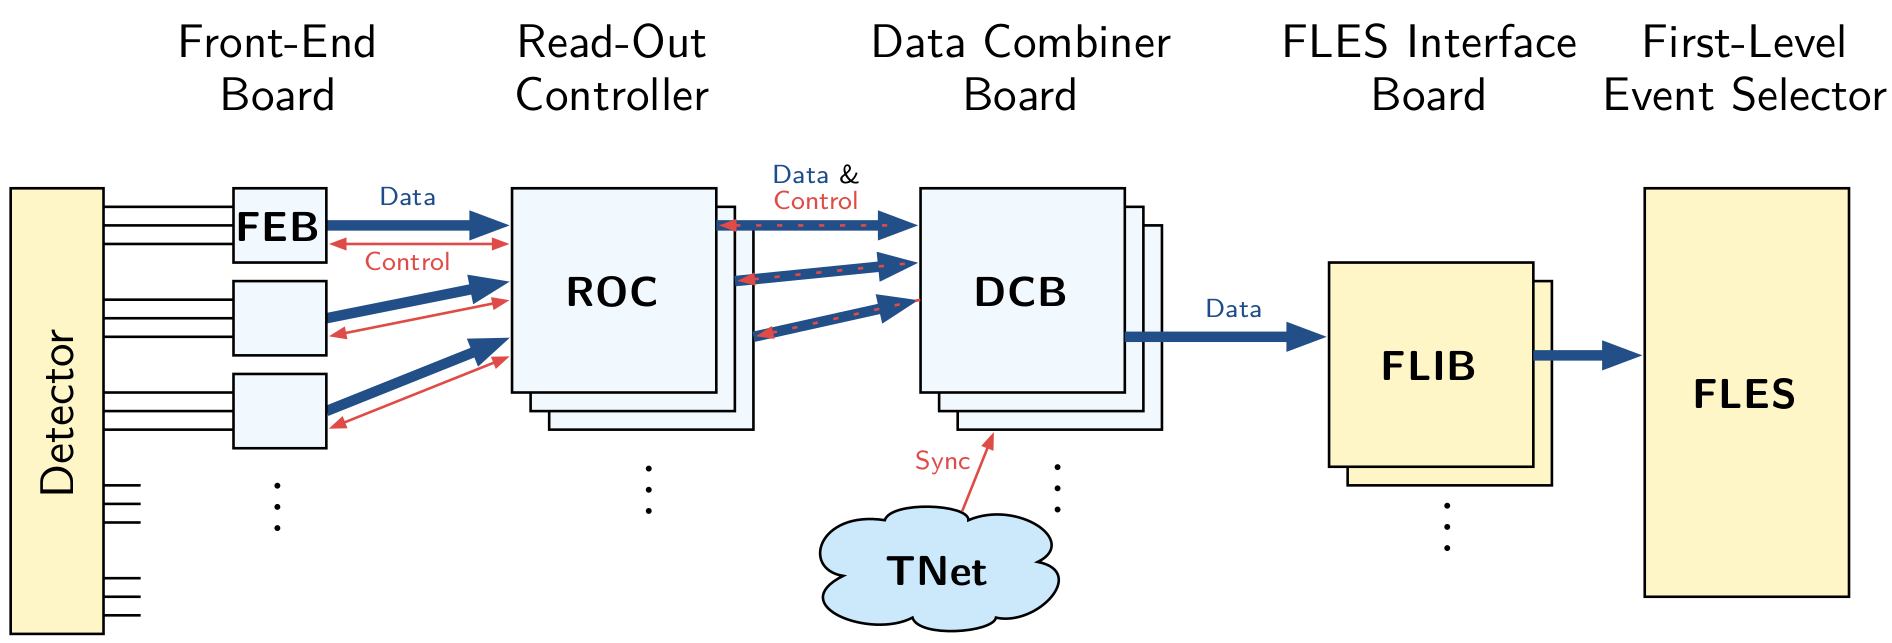
\includegraphics[width=0.7\textwidth]{pictures/CBMreadout.png}
\caption{Система считывания и сбора данных CBM.}
\label{fig:CBMreadout}
\end{figure}

\textbf{Развёрнутое описание выше делается для понимания этой секции.}

Источником электрических сигналов являются детекторы, выполненные по разным технологиям, и требующие оцифровки различными способами. Эта оцифровка выполняется разнообразными платами передней электроники (FEB), имеющими разные принципы и основанными на различных чипах. Затем цифровые данные опрашиваются с плат передней электроники контроллерами считывания (ROC). После этого данные группируются в соответствующих платах (DCB) и поступают во FLES через платы FLIB.

\subsection{FLES}\label{sec:secFLES}

\textbf{переработать}
Всё вместе привело к разработке аппаратно-программного комплекса, называемого системой отбора первого уровня --- First Level Event Selector (FLES). По сути DAQ-часть (приём данных) неотделима от FLES, поэтому иногда эту систему называют FLES/DAQ.
Отличительные черты FLES --- самотриггирующаяся электроника, несколько уровней концентрации данных, многочисленные буферы, формирование срезов времени, построение интервалов и только после этого мы переходим к построению событий.

% 1 - Приём данных и формирование срезов времени
Функционал FLES/DAQ можно разбить на три части. Первая --- приём и объединение данных, поступающих с группы каналов, в срезы времени (timeslice). Такую группу образует некоторое множество каналов одного детектора, количество которых определяется ожидаемым потоком данных, а ограничение диктуется максимальной пропускной способностью входного канала FLES.

% 2- Interval building
Один из наиболее важных и нестандартных этапов работы FLES --- это построение интервалов (Interval building, IB). Построение интервалов --- это получение контейнеров с данными со всех детекторов за некоторый интервал времени путём перегруппировки данных из срезов времени. Суть построения интервалов показана на \figref{fig:IntervalBuilding}. Данные от одного ``входного узла'' (input node, IN) приходят от группы каналов какого-то детектора и представляет собой последовательность срезов времени. Задача заключается в том, чтобы объединить все срезы, соответствующие одному интервалу времени, чтобы дальше передать на ``вычислительный узел'' (processing node, computing node, CN).

\begin{figure}[H]
\centering
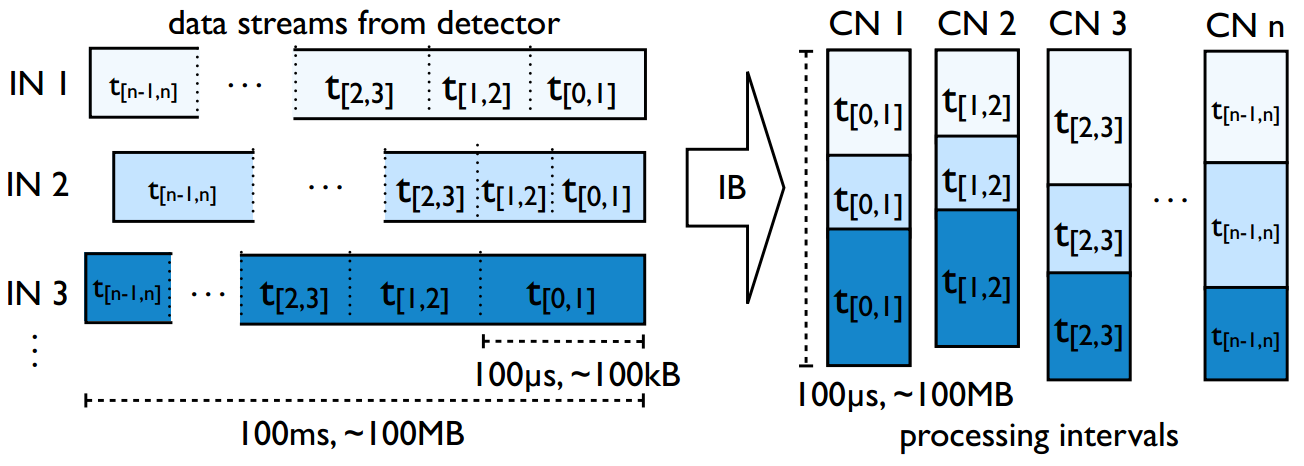
\includegraphics[width=0.7\textwidth]{pictures/Interval_building.png}
\caption{Построение интервала.}
\label{fig:IntervalBuilding}
\end{figure}

% 3- Этап после построения интервалов
Заключительный этап обработки данных во FLES --- восстановление событий в интервале, реконструкция треков и частиц в восстановленных событиях и выработка сигнала о сохранении или отбросе интервала.

% Численные оценки, определение FLES как сети из узлов
Для эксперимента CBM был выполнен оценочный расчёт. Отправная точка --- возможно сохранение 1~Гбайт/сек данных. Считается, что одно событие CBM в среднем имеет объём 40~Кбайт. Отсюда следует, что максимальная частота первичного взаимодействия может быть 25~кГц. В стартовой конфигурации CBM частота первичного взаимодействия равна 10~МГц, следовательно, необходимо уменьшить поток данных в 400~раз. В полноценном режиме работы CBM ожидается 25~МГц, т.е. $ 25 \cdot 10^{6} \cdot 40 $ Кбайт = 1 Тбайт/сек. Планируется разбить этот поток в 1~Тбайт/сек на 1000 входных каналов FLES, каждый по 1~Гбайт/сек, передающихся по 10-Гбитным оптическим каналам связи. Один входной канал FLES соответствует одному ``входному узлу'' --- ЭВМ с установленной платой FLIB. Все вычисления, необходимые для отбора данных будут осуществляться на так называемых ``вычислительных узлах''. Входные и вычислительные узлы объединены в компьютерную сеть посредством InfiniBand QDR, образуя уникальную распределённую вычислительную систему, называемую FLES, см. \figref{fig:FLESarch}. Вычислительная подсеть будет иметь приблизительно 60000 ядер.

\begin{figure}[H]
\centering
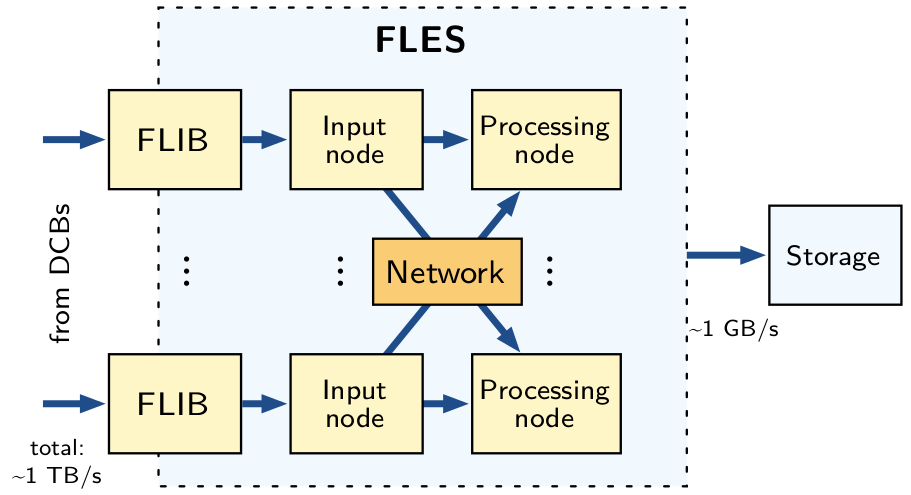
\includegraphics[width=0.7\textwidth]{pictures/FLESarch.png}
\caption{Общая схема устройства FLES.}
\label{fig:FLESarch}
\end{figure}

% Реконструкция по одному детектору
Планируется также, что FLES сможет функционировать в особом режиме, когда для выполнения реконструкции с целью отбора данных для сохранения будет использоваться только часть входного потока. На \figref{fig:PartialIB} приведена блок-схема функционирования FLES в таком режиме. Это имеет смысл при работе эксперимента над некоторыми пунктами физической программы, но принципиальная возможность и эффективность реконструкции частиц с целью триггирования по ограниченному набору детекторов является предметом исследований. Например, можно восстанавливать \todo такую-то частицу только по трекам в MUCH. При этом система приёма данных работает в полную силу --- идёт приём со всех детекторов и никакие данные не выбрасываются до тех пор, пока не будет выполнена реконструкция по данным с MUCH. Если в результате реконструкции выясняется, что принятая порция данных потенциально интересна, то она извлекается из буферов и записывается. Это позволяет \todo снизить поток сохраняемых данных в \todo раз, что особенно актуально при экстремально высоких частотах взаимодействия.

\begin{figure}[H]
\centering
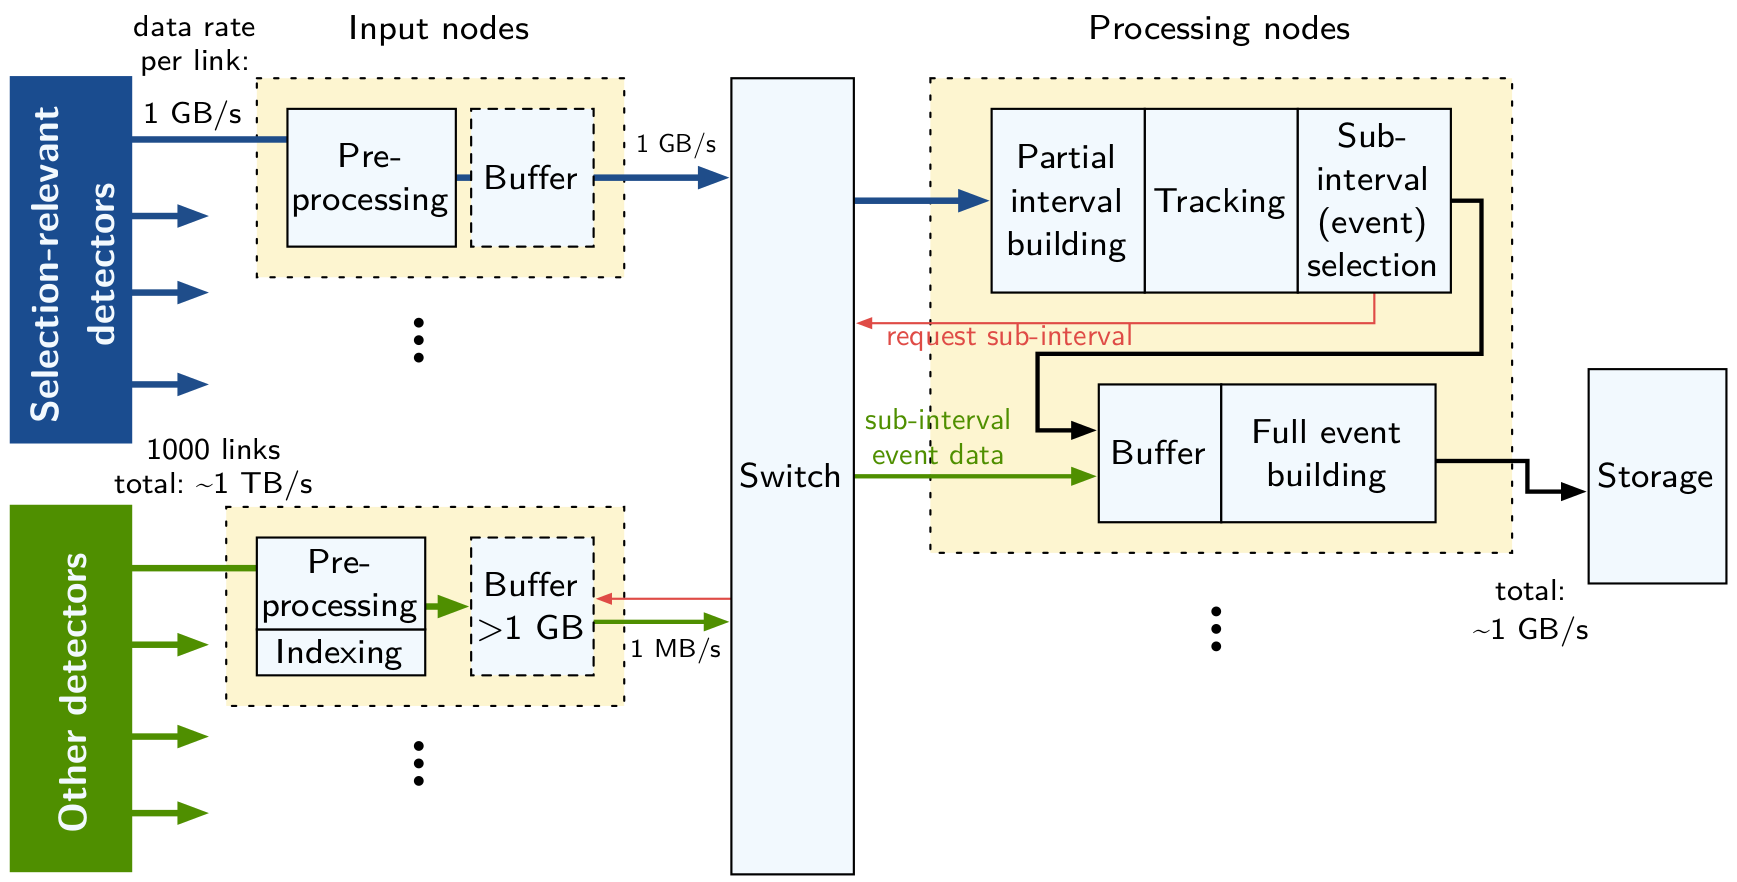
\includegraphics[width=1.0\textwidth]{pictures/PartialIB.png}
\caption{Блок-схема функционирования FLES в режиме отбора по данным с части детекторов.}
\label{fig:PartialIB}
\end{figure}

\todo Подробное описание того, что на картинке

% FLIB
\subsubsection{FLES Interface Board}\label{sec:FLIB}

В качестве платы-интейфейса между электроникой, разрабатываемой специально для CBM, и ЭВМ стандартной архитектуры, будет выступать плата, в общем называемая платой интерфейса FLES --- FLES Interface Board, или FLIB. FLIB можно рассматривать как особый сетевой интерфейс, основной задачей которого является предоставление данных, поступающих по входным каналам, центральному процессору ЭВМ. В отличие от сетевого интерфейса Ethernet, данные поступают от разнородных плат передней электроники по разным протоколам. В качестве платформы для реализации FLIB в CBM рассматривается коммерческая PCI-E плата HTG~K-7. Архитектура FLIB показана на \figref{fig:FLIBarch}. Основные компоненты FLIB --- драйверы входных оптических портов, программируемая пользователем вентильная матрица (ППВМ, FPGA), оперативное запоминающее устройство (ОЗУ) и драйвер шины PCI-Express. 

\begin{figure}[H]
\centering
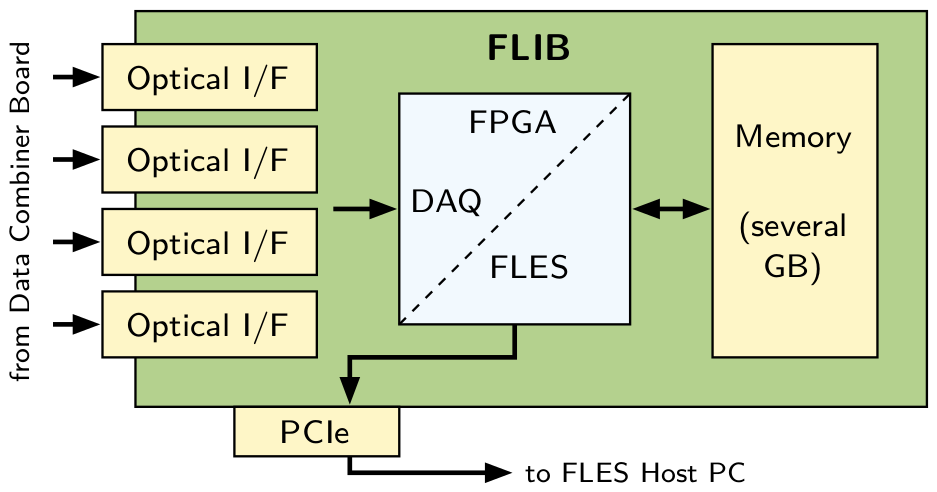
\includegraphics[width=1.0\textwidth]{pictures/FLIBarch.png}
\caption{Архитектура FLIB.}
\label{fig:FLIBarch}
\end{figure}
